\chapter{Data Anaysis}
\section{Analysis Summary}
This analysis uses the data collected during the \sqrtsNN{} = 5 TeV \pPb~run in 2013 and during the \sqrts{} = 5 TeV pp run in 2017. The EMCal trigger was used to select events with a high-momentum calorimeter cluster, a photon \pt range of {12--40 \GeVc}.%, equivalent to $x_{\mathrm{T}} = 2\pt/\sqrt{s_{\mathrm{NN}}}$ in the {0.006--0.012} range.  %The thresholds of the trigger corresponds to about {$\pt$ = 7 and 11 \GeVc} in the \pPb~data and about {5 \GeVc} in the pp data.

The signal for this analysis, is ''prompt'' photons, which include ''direct photons'' and ''fragmentation photons''. At leading order in perturbative QCD, the direct photons are produced in hard scattering processes such as quark-gluon Compton scattering ($qg\to q\gamma$) or quark-antiquark annihilation ($q\bar{q}\to g\gamma$), whereas the fragmentation photons are the product of the collinear fragmentation of a parton ($q\bar{q}(gg)\to \gamma + X$). At LHC energies, Compton scattering and gluon fusion $(gg\to  q\bar{q}\gamma)$ dominate due to the high-gluon density in the proton at small values of Bjorken-$x$. 

Beyond the simplistic leading order picture, the direct and fragmentation components have no physical meaning and cannot be factorized; the sum of their cross sections is the physical observable. For example, the separation between the NLO direct photons and LO fragmentation is arbitrary. However, it is still possible to simplify comparisons with theoretical calculations by applying an isolation criteria. The isolation variable used is the sum of the transverse momentum of the charged particles that are inside an angular cone of radius $R =\sqrt{(\Delta\phi)^{2} +(\Delta\eta)^{2}  } =0.4$ around the photon direction, after subtracting the underlying event. 

The main background for this analysis are photons from meson decays, which we will call ''decay photons'' or $\ydecay$. The  challenge faced in this measurement arises mainly from the small cross-section of the signal compared to that of the decay photon background (about 1$\%$ at {10 \GeVc} increasing to about 4$\%$ at {30 \GeVc}, according to next-to-leading order calculations~\cite{Arleo:2004gn}). 

This measurement exploits the difference between the electromagnetic shower profiles of prompt photons and of photon pairs from neutral-meson decays. The clusters that pass the isolation and shower shape selections isolated $\gamma$ candidates or ''\gammaiso candidates''. 

The main background in within the $\gammaiso$ candidate population are from multi-jet events where one jet typically contains a $\pi^{0}$ or $\eta$ that carries most of the jet energy and is misidentified as a photon because it decays into a photon pair that is collinear with respect to the EMCal cell granularity ($\Delta\eta\times\Delta\phi\approx$  14.3$\times$14.3 mrad$^{2}$), that is, the two photons are close enough to deposit most of their energy in the same cell and appear as a single shower. 

The signal purity of the $\gammaiso$ selection is measured by using the ''template-fit method'', in which the measured shower-shape distribution is fit with the sum of signal and background templates with the relative normalization as the single free parameter\footnote{Note that this is an standard way to estimate QCD background since at least the Tevatron days. The same exact method is used in the CMS $\gammaiso$ and $\gammaiso$--jet measurements in pp and PbPb data, for example in Refs.~\cite{Sirunyan:2018gro,Chatrchyan:2012gt}.}. The background template is mostly data-driven, calculated with an anti-isolated sideband requirement, but a MC-based correction is applied to account for estimated biases. The signal template is obtained from photon-jet simulation. The purity of our $\gammaiso$ selection is measured to be around 20$\%$ at {12 \GeVc} and increases to about 55$\%$ at {20 \GeVc} and above. 

Next, the angular correlation of the $\gammaiso$ candidates with charged particles is measured.  The {$\ydecay$--hadron} correlation function is measured by inverting the shower-shape cut to select merged-clusters from meson decays, and is called the \textit{Background Region} correlation function. Both the signal and background region photon-hadron correlations are corrected for geometrical pair acceptance effects using the mixed-event technique. Afterwards, the $\ydecay$--hadron correlation is normalized using the measured purity and subtracted from the normalized the main $\gammaiso$ candidate correlations in a process labelled "correlated background subtraction".

After this correlated background subtraction, the uncorrelated background, estimated by the zero-yield-at-minimum (ZYAM) method and checked by using a control region at large $|\eta^{\mathrm{hadron}}-\eta^{\gamma}|$ is subtracted from the main $\gammaiso$ candidate correlation function. Finally, the away-side of the resulting correlation function is integrated to determine the number of correlated hadrons per $\gammaiso$, i.e. to measure the conditional yield of hadrons. This analysis is performed with photons with $12<\pt <40~\GeVc$, and in intervals of charged particle \pt~and $\zt \equiv \pth/\ptgamma$. 

%We also present an $\gammaiso$--jet analysis. We reconstruct jets with the anti-$k_{\mathrm{T}}$ algorithm on tracks with {$0.15$ $<\pt < 15$ \GeVc} and $|\eta|<0.8$ as input. We select jets with {$\pt>$ 10 \GeVc} recoiling against the $\gammaiso$ candidate (with $|\phi^{\mathrm{jet}}-\phi^{\gamma}|>\pi/2$) and measure the angular correlations and momentum balance, and we also explore measurements sensitive to jet-flavor. To subtract the $\ydecay$--jet background arising from the impurity of our $\gammaiso$ candidate selection, we invert the shower-shape cut to select merged-clusters from meson decays and measure the corresponding background distributions, properly scaled by the purity of our $\gammaiso$ selection. We also subtract uncorrelated background, i.e correlations with jets produced by underlying event, by estimating it using event-mixing. The final $\gammaiso$--jet results are compared with $\pi^{0}$--jet correlations and \textsc{Pythia} photon+jet simulations at the reconstructed level and at particle level, i.e. after unfolding the jet detector smearing.

%The ratios of the p-Pb and pp distributions are compared to next-to-leading order perturbative quantum chromodynamic calculations with proton and nuclear parton distribution functions. While this measurement turns out to be dominated by statistical uncertainties, it still constrains the gluon densities in nuclei in the poorly explored low-$x$ and low-$Q^{2}$ region. This measurement also constitutes a benchmark for photon identification, background subtraction, and jet reconstruction for future measurements with larger data samples of proton-lead and lead-lead collisions. 

One of the novel aspects of this analysis is the use of ITS standalone tracking. This approach was developed in order to bypass the serious space-charge distortions that compromised the TPC during the high-luminosity \pPb~data taking in 2013\footnote{For details, see \url{https://alice.its.cern.ch/jira/browse/ATO-351}, \url{https://alice.its.cern.ch/jira/browse/PWGPP-349},
\url{https://alice.its.cern.ch/jira/browse/PWGPP-314}
}. Furthermore, the ITS-only tracking allowed the 2017 pp run to operate in the CALO mode that yielded a much larger sample than would have been possible otherwise. 

The performance of the ITS-standalone tracking (fake rate, efficiency and momentum smearing) was validated by measuring the charged particle spectrum and comparing it with published ALICE measurements at the same center-of-mass energy. These studies showed an agreement between the ITS-standalone measurement and the published data to within $\approx \pm 5\%$ of the corresponding published data for the range {$0.5<\pt<10$ \GeVc}, which is the relevant range in this analysis. 

One of the main considerations of the larger analysis strategy was to minimize the use of Monte Carlo simulations. By using an isolation variable constructed using only charged particles, the correlations between isolation and shower-shape variables due to the opening angle of neutral-meson decays has been reduced, at the expense of a slightly lower purity. In the template fit analysis, checks were performed that are independent of any input from simulations, suggesting the template fit is not sensitive to the detailed simulation of the exact shower-shape distributions. Moreover, the analysis measures per-trigger quantities such that there is no need to correct for the efficiency of the $\gammaiso$ selection. %While we use Monte Carlo simulations to construct the response matrices used in the unfolding of the detector response for jet measurements, these are validated with {\it in situ} calibrations of the jet energy scale. Therefore, detailed studies of multidimensional comparisons of data and simulations are not needed for this analysis, and are skipped in this note. 

While an effort was made to collect and use the largest data samples available by pioneering high-rate data taking with ITS+EMCal, the measurement turns out to be dominated by statistical uncertainties. Faced with this reality, efforts to reduce the systematic uncertainties of the measurement were tempered such that they are smaller than the statistical uncertainty.

\section{Datasets}
\label{sec:datasets}
The datasets used in this analysis include the high-luminosity runs of the 2013 \pPb~run (13d,e,f) and the 2017 pp run (17q) that were collected with EMCal triggers, which are listed in Table~\ref{tab:triggerstrings}.  

\begin{table}[h]
    \centering
    \caption{EMCal triggers used in this analysis.}
   \label{tab:triggerstrings}
   \begin{tabular*}{1.0\columnwidth}{@{\extracolsep{\fill}}ll@{}}
        \hline
        Dataset &  Trigger Strings\\
        \hline
        \pPb & CEMC7EG1-B-NOPF-CENTNOTRD, CEMC7EG2-B-NOPF-CENTNOTRD,\\
        \hline
        pp & CEMC7EG2-B-NOPF-CALO, CDMC7DG2-B-NOPF-CALO,\\ 
           & CEMC7EG2-B-NOPF-CENT,	CDMC7DG2-B-NOPF-CENT\\
        \hline
   \end{tabular*}
\end{table}


The EMCal gamma trigers (EG1, EG2, DG1, DG2) are based on the summed energy in 2$\times$2 adjacent tiles (a tile is composed of an EMCal module, 2$\times$2 adjacent cells). The trigger thresholds were 7 and 11 \GeVc~during the 2013 \pPb~run and {5 \GeVc} during the 2017 pp run. %The EMCal jet (EJ1, EJ2) triggers are based on a patch of 32 $\times$ 32 adjacent towers, corresponding to an area of approximately 0.2 rad was used. This jet patch trigger fired if an integrated patch energy of at least 10 GeV (low-energy trigger) or 20 GeV (high-energy trigger) was found.

Due to the 2-in-1 magnet design of the LHC, which requires the same magnetic rigidity for both colliding beams, the beams had different energies during the \pPb~run ({$E_{\mathrm{p}}$ = 4 TeV}, {$E_{\mathrm{Pb}} $= 4 TeV$\times$Z}, where $Z=82$ is the atomic number of lead). In the lead nucleus, the energy per nucleon was therefore  {$1.56$ TeV $= (Z/A) \times$ 4 TeV}, where $A =$ 208 is the nuclear
mass number of the lead isotope used. This energy asymmetry results in an average nucleon--nucleon center of mass collision energy of {$\sqrt{s_{\mathrm{NN}}}=5 $ TeV} and a rapidity boost of this frame by $\pm$0.465 units relative to the ALICE rest frame in the direction of proton beam. Around halfway through the 2013 \pPb~run, the beam directions were flipped, yielding similar integrated luminosities in both beam configurations. %Following an established convention, we report pseudorapidity in the nucleon-nucleon collision frame, $\eta^{*}$, with a positive (negative) pseudorapidity corresponding to production in the downstream proton (downstream nuclear) beam direction. Therefore, a massless particle emitted at $\eta_{\mathrm{cm}}=0$ in the nucleon-nucleon center-of-mass frame will be detected at $\eta_{\mathrm{lab}}=$+0.465 in the laboratory frame.  

%%%%%%%%%%%%%%%%%%%%%%%%%%%%%%%%%%%%%
During the 2013 \pPb~run period, the TPC suffered from space-charge distortions\footnote{For more information on the problems with space-charge distortions due to high-luminosity in \pPb~run, see: https://alice.its.cern.ch/jira/browse/PWGPP-314.} that affect tracking, leading to a very drastic drop in efficiency for tracks with $\pt> 4$ \GeVc. We bypass this issue by using ITS-only tracking as detailed in Section~\ref{sec:tracking}.
For the 2017 pp data, the TPC was also inactive due to the high luminosity of the runs considered in this analysis. We use the 17q period, during which all six layers of the ITS were active.

The average number of inelastic collisions per bunch crossing, $\mu$, is 0.020--0.060 for the 2013 \pPb~data set and in the range 0.015--0.045 for the 2017 pp dataset~\footnote{This information can be found in \url{http://aliqaevs.web.cern.ch/aliqaevs/data/2013/LHC13d/pass4/global_properties.pdf} and \url{http://aliqaevs.web.cern.ch/aliqaevs/data/2017/LHC17q/cpass1_pass1/global_properties.pdf}}.% Thus, one expects an in-time pileup, i.e. multiple collisions in the same bunch crossing at the level of less than 1$\%$ (given by the Poisson probability of $P(n>1) = 1-P(n=0) = e^{-\mu})$. 

%Figure~\ref{fig:RejectionFactorpPb} shows the rejection factor of the EMCal gamma triggers. The curves already reached a plateau for clusters with $\pt=12$ \GeVc, which is the minimum $\pt$ used in this analysis. 

%%\begin{figure}[h]
%\center
%\includegraphics[width=0.6\textwidth]{Datasets/RejectionFactorpPb2013}
%\caption{Rejection factor curves for the 2013 p-Pb period (13def). Source: Ref.~\cite{Erwann}.}
%\label{fig:RejectionFactorpPb}
%\end{figure}


%The total integrated luminosity of the 2013 p-Pb sample is about {4.6 nb$^{-1}$} {($\times$ $A$ = 967 nb$^{-1}$ pp equivalent luminosity)} and about {300 nb$^{-1}$} for the 2017 pp sample. Note that the DCal increases the geometrical acceptance for photons by roughly a factor of 1.3; therefore, comparable statistics of high-$\pt$ photons are expected for pp and p-Pb data.~\footnote{This is the first hard-probes analysis in ALICE that has similar statistics in the reference pp data at the same center-of-mass energy, and thus does not need to rely on extrapolations.}



\section{Monte Carlo simulations}
\label{sec:mcsimulations}
We use Monte Carlo (MC) simulations to obtain the signal shower-shape distributions for the template fits (section~\ref{sec:purity}) and to study tracking performance (section~\ref{sec:tracking}).

The simulations of hard processes are based on the \textsc{Pythia} event generator. In \textsc{Pythia}, the signal events are included via $2\to2$ matrix elements with $gq\to\gamma q$ and $q\bar{q}\to\gamma g$ hard scatterings, defined at the leading order, followed by the leading-logarithm approximation of the partonic shower. The soft underlying events in pp collisions as well as fragmentation are included with the default \textsc{Pythia} models. 

For the simulation of \pPb~events, the pp samples are embedded into \pPb~inelastic events generated with \textsc{DPMJET}. The boost of $\Delta y=+0.465$ in the direction of the proton beam is reproduced. % to reproduce the experimentally measured global \pPb~event properties. 

% Table~\ref{tab:MCsamples} shows the MC simulations used in this analysis. Each sample is simulated with the detector configuration appropriate for the runs used in this analysis. 

% \begin{table}[h]
%    \centering
%    \caption{Monte Carlo simulations used in this analysis.}
%    \label{tab:MCsamples}
%    \begin{tabular*}{1.0\columnwidth}{@{\extracolsep{\fill}}llcc@{}}
%     \hline
%         Name  & Configuration & JIRA ticket link \\
%         \hline        
%  17g6a1	 &\pPb, 5 TeV, \textsc{Pythia8} Gamma-Jet +DPMJET anchored to 13d,e,f& \href{https://alice.its.cern.ch/jira/browse/ALIROOT-7271}{ALIROOT-7271}\\
%  17g6a3	 &\pPb, 5 TeV, \textsc{Pythia8} Jet-Jet +\textsc{DPMJET} anchored to 13def& \href{https://alice.its.cern.ch/jira/browse/ALIROOT-7271}{ALIROOT-7271}\\
%   13b2    &\pPb, 5 TeV, \textsc{Dpmjet} anchored to LHC13b,c & \href{https://alimonitor.cern.ch/productions/3996/tag.html}{39374}\\
%  18b10a(b)\_calo	 &pp 5 TeV, \textsc{Pythia8} Gamma-Jet anchored to 17p/q& \href{https://alice.its.cern.ch/jira/browse/ALIROOT-7692}{ALIROOT-7692}\\
%  18l2a(b)     &pp 5 TeV, \textsc{Pythia8} Jet-Jet anchored to 17p/q& \href{https://alice.its.cern.ch/jira/browse/ALIROOT-8144}{ALIROOT-8144}\\
   
%                  \hline
%    \end{tabular*}
% \end{table}


\section{Event Selection}
\label{sec:eventselection}
The following event selection criteria is used to ensure good event quality and uniform acceptance:
\begin{itemize}
\item Run passes QA for EMCal and ITS (the selected runs are listed in Table~\ref{tab:datasets}).
\item At least one EMCal cluster with $\pt>12$ \GeVc.
\item Selected at least one of the EMCal triggers (logical OR of the trigger strings listed in Table~\ref{tab:triggerstrings}).  %(low and high thresholds).
\item Valid vertex ($|z|\neq0.0$) and $|z|<10$ cm 
%\item Pileup rejection (\textsc{IsPileupFromSPD}(5, 0.8)=False).
\end{itemize}

Where the EMCal is mentioned, we use the same criteria on the DCal (used in the 17q dataset). We use EMCal in text for brevity.
The number of events that pass our selection in each sample is shown in Table~\ref{tab:eventsselected}. We report the events selected for each trigger separately, as well as the logical OR combination. In \pPb~events, the number of events is dominated by the EG1 trigger (11 \GeVc~thrshold), and by the EG2 trigger (5 \GeVc) in pp collisions. 

\begin{table}[h]
   \centering
   \caption{Number of events that passed our full event selection for each of data taking period used in this analysis. The numbers are also shown separately for EG1 (DG1) and EG2 (DG2) triggers.}
   \label{tab:eventsselected}
   \begin{tabular*}{1.0\columnwidth}{@{\extracolsep{\fill}}llll@{}}
    \hline
    Dataset &  	N$^{\mathrm{EG1||EG2}}$ &	N$^{\mathrm{EG1}}$ & N$^{\mathrm{EG2}}$\\
    \hline
    13d &	134024 & 133326 & 12528\\
    13e &	198108 & 196745 & 22409\\
    13f &   340607 & 338198 & 38353\\
    13f\_new & 241870 & 240074 & 30310\\
%    Dataset &  	N$^{\mathrm{EG1||EG2||EJ1||EJ2}}$ &	N$^{\mathrm{EG1}}$ & N$^{\mathrm{EG2}}$ &	N$^{\mathrm{EJ1}}$  &	N$^{\mathrm{EJ2}}$ \\
%    \hline
%    13d &	173583 & 133326 & 12528 & 122168 & 20917\\
%    13e &	206833 & 196745 & 22409 & 167651 & 3063\\
%    13f &   365775 & 347684 & 40133 & 296144 & 6501\\
%    13f\_new & 252738 & 240074 & 30310 & 204298 & 5110\\
    \hline
    Dataset &	N$^{\mathrm{EG2 || DG2}}$ &		N$^{\mathrm{EG2}}$ & N$^{\mathrm{DG2}}$\\
    \hline

    17q & 406934 & 301086 & 119498 \\
 
    \hline
   \end{tabular*}
\end{table}

\section{Calorimeter cluster reconstruction}
\label{sec:clusterselection}
\subsection{Definition}
EMCal clusters are formed by a clustering algorithm that combines signals from adjacent towers. We use calorimeter clusters defined with the ``V1'' algorithm. This algorithm starts from a ``seed" cell, found from a local-maximum scan, and adds ``neighbor" cells to the cluster if they are above a given threshold. The cluster definition is exclusive, i.e. once a cell is assigned to a cluster, it is not considered for other clusters. The minimum energy for the seed and neighbor were set to 500 and 100 MeV respectively; these values are several times larger than the standard deviation of the electronic noise\footnote{Some photon analysis use a 50 MeV threshold, but 100 MeV has been found to improve cell time measurements. The 100 MeV threshold has been used for example in Ref~\cite{Acharya:2017tlv}.}.

\subsection{Corrections}
We apply several corrections at the cell level, implemented within the ``EMCal Correction Framework,"\footnote{\url{http://alidoc.cern.ch/AliPhysics/master/_r_e_a_d_m_eemc_corrections.html} } before the clustering algorithm is run over the data and simulations. The following corrections are applied: 
\begin{itemize}
\item ``\textsc{CellEnergy}"\\
This performs an energy calibration of cells, with coefficients obtained with $\pi^{0}\to\gamma\gamma$ mass measurements.
\item ``\textsc{CellBadChannel}''\\
This removes cells that declared hot or dead for a given run period. 
\item ``\textsc{CellTimeCalib}"\\
This correction applies constant offsets, which are arbitrary, to the cell time measurements to minimize the spread among cells. 
\item ``\textsc{CellEmulateCrosstalk}''. \\
This correction, described in detail in Ref~\cite{CrossTalk}, modifies the simulated cell energies to emulate the cell cross-talk that has been observed in data. This is applied to all the simulations described in Table~\ref{tab:MCsamples}. 
\end{itemize}

\subsection{Selection}
The following selection is applied on the resulting clusters\footnote{This event selection also closely follows previous and concurrent isolated-photon spectra analyses in pp and \pPb~ data.}:

\begin{itemize}
\item Cluster $\pt$ cut:  $12< \pt < 40$ \GeVc.
\item Cluster pseudorapidity: $|\eta| <0.67$\\
The cluster pseudorapidity is corrected for the position of the primary interaction vertex. 
\item Number of cells cut: $N_{\mathrm{cell}}\geq2$\\
This requirement removes clusters that are likely dominated by noise. 
\item Exoticity cut: $E_{\mathrm{cross}}/E_{\mathrm{cluster}}$ $> 5\%$\\
We remove ``exotic'' or ``spiky'' clusters likely coming from slow neutrons or highly-ionizing particles hitting the avalanche photo-diode of a cell by a requirement on the ratio of the summed energy around the leading cell to the total cluster energy.
\item Cluster time cut:  $|t|<20$ [ns]\\
We require a cluster time measurement of $|t|<$ 20 ns to remove out-of-bunch pileup. 
\item Number of local maxima cut: $N_{LM}<$ 3\\
This cuts suppresses background and improves the MC simulation description of the background~\cite{Acharya:2019jkx}.  
\item Distance seed-cell to bad-channel$\geq 1$ cells.
\end{itemize}

Figures~\ref{ClusterCutFlow_pPb} and~\ref{ClusterCutFlow_pp} show the distribution of the variables used in the cluster selection and the effect of sequential selection (``cut flow") for the \pPb~and pp data respectively. Table~\ref{tab:photonCutFlow} shows a summary of the effect of sequential selection on the number of selected clusters in both pp and \pPb~data. 

\begin{figure}[h]
\center
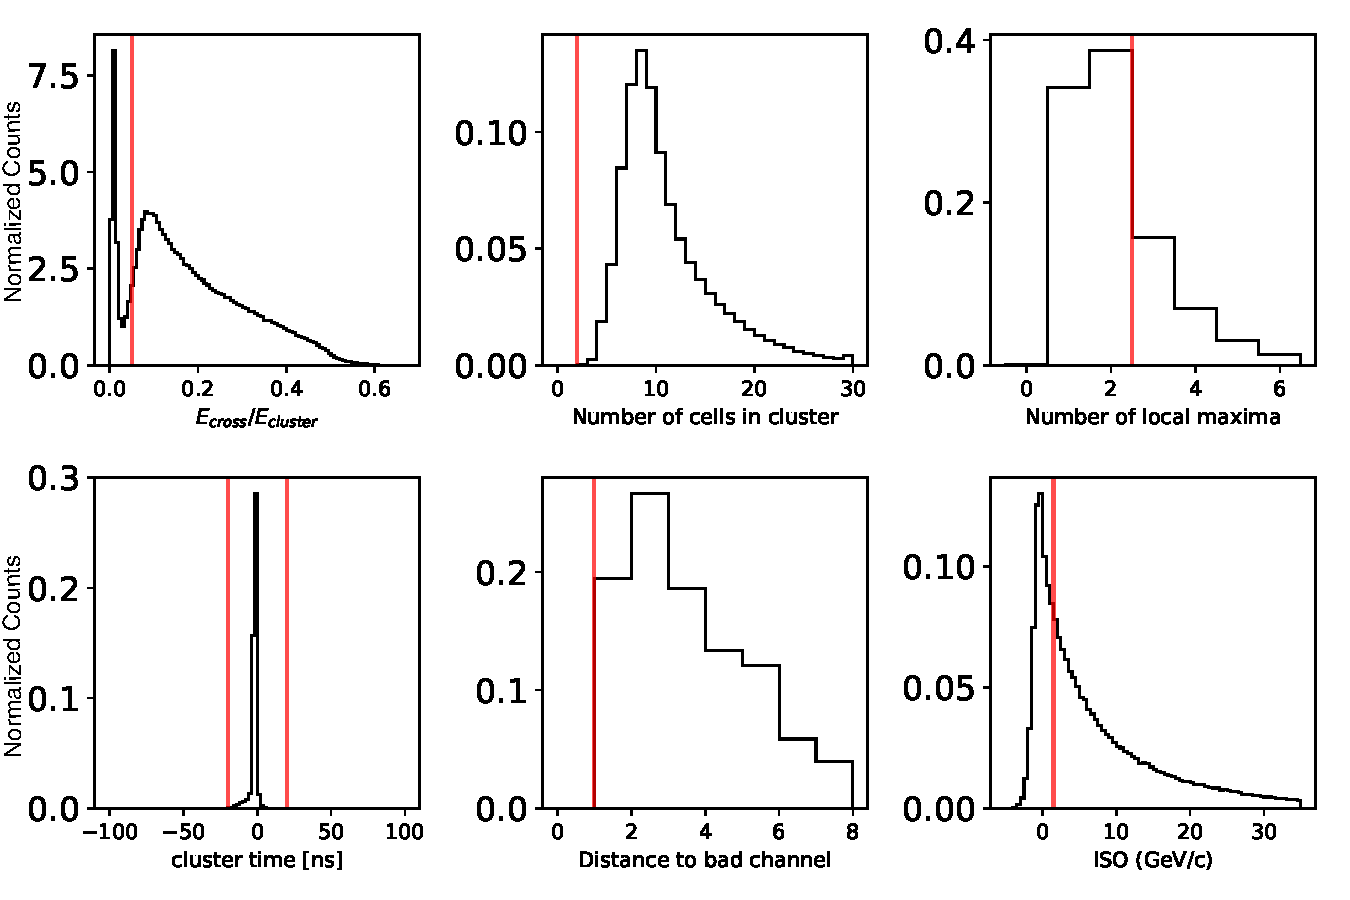
\includegraphics[width=0.95\textwidth]{Data_Analysis/EventAndClusterSelection/ClusterCutFlow_dataset_Skimmed_13def}
\caption{Distribution of variables used in the cluster selection of \pPb~data. The red vertical lines represent the cuts used. The cluster cuts get applied sequentially, i.e. the clusters cut with a given variable do not appear in the next.}
\label{ClusterCutFlow_pPb}
\end{figure}


\begin{figure}[h]
\center
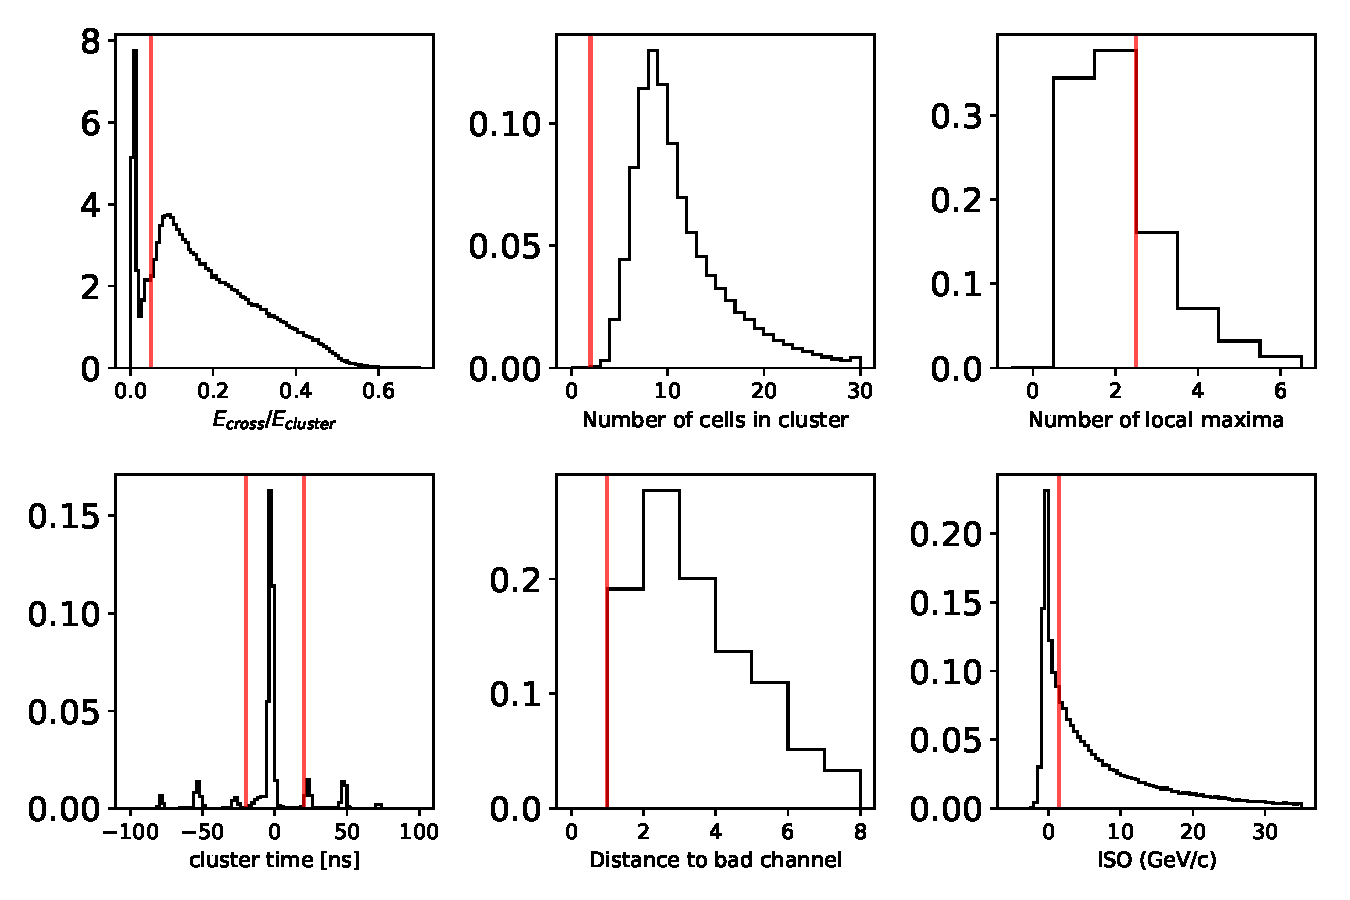
\includegraphics[width=.95\textwidth]{Data_Analysis/EventAndClusterSelection/ClusterCutFlow_dataset_Skimmed_17q}
\caption{Distribution of variables used in the cluster selection in pp data. The red vertical lines represent the cuts used. The cluster cuts get applied sequentially, i.e. the clusters cut with a given variable do not appear in the next.}
\label{ClusterCutFlow_pp}
\end{figure}


\begin{table}[h]
   \centering
   \caption{Number of clusters, with  $12<\pt<40$ \GeVc, that pass our selection in 2013 \pPb~and 2017 pp data.}
   \label{tab:photonCutFlow}
   \begin{tabular*}{1.0\columnwidth}{@{\extracolsep{\fill}}lcc@{}}
    \hline
       Selection  &  \pPb~ data & pp data  \\
       \hline
       $|\eta| < 0.67$& 714834 & 385220  \\
      $E_{\mathrm{cross}}/E_{\mathrm{cluster}}$ $> 5\%$ & 613560 & 323750   \\
       $N_{\mathrm{cell}}$ $\geq 2$   &613560& 323750       \\
              $N_{LM}<$ 3 & 443102&231490 \\
       $|t|<20$ [ns] &441639 & 171470  \\ 
       Distance-to-bad channel $\geq 1$ &441639  &171470  \\ 
       $\iso<$  1.5~\GeVc & 137895  & 58638 \\ 
       0.1 $< \sigma^2_{\textrm{long}}<$  0.3  & 40027 & 16628  \\ 
       \hline
	   %Total clusters passing $\gammaiso$ selection & 38415  & 16,586 %\\ 
       %\hline
   \end{tabular*}
\end{table}

\FloatBarrier

\section{Isolated Prompt Photon Selection} 
\label{sec:photons}

A key challenge of this measurement is the relatively small cross section of prompt photons compared to decay photons. In order to reduce the background of decay photons, and to identify prompt photons, a combination of isolation and electromagnetic shower profile selections are made. Photons are observed in their final state as an reconstructed cluster in the calorimeter. Clusters are obtained by grouping all adjacent cells with common sides whose energy is above {100 MeV}, starting from a seed cell with at least {500 MeV}. Furthermore, a cluster must contain at least two cells to remove single-cell electronic noise fluctuations. Clusters are required to have a minimum \pt of \ptgamma $\geq 12$ \GeVc. The time of the highest-energy cell in the clusters relative to the main bunch crossing must satisfy $\Delta t < 20$ ns to reduce out-of-bunch pileup. In order to limit spurious signals caused by particles hitting the EMCal APDs, clusters are required to have $E_{\mathrm{cross}}/E_{\mathrm{cluster}}>0.05$, where $E_{\mathrm{cross}}$ is the sum of the energy in the cells adjacent to, but not including, the leading cell, and $E_{\mathrm{cluster}}$ is the total energy of the entire cluster. The number of local maxima in the cluster is required to be less than three to reduce hadronic background. To select against photons from neutar-meson decays or fragmentation processes, a shower profile selection and isolation requirement are applied to these clusters. 

%Also included in the definition of direct photons are thermal photons. These photons are produced as thermal radiation emitted by the quark gluon plasma. Thermal photons dominate the direct photon spectrum at low \pt, and at energies much lower than the photons of interest in this measurement (Section \ref{sec:photon_selection}).

\subsection{Shower Profile Selection}
The primary background for this measurement are photons from the 2-body decay channel of neutral mesons $\pizero$'s. A \pizero~with a higher \pt will decay  with a smaller opening angle between the two decay photons. As the opening angle becomes smaller, the electromagnetic showers from the decay photons get closer together in the EMCal until they begin to overlap. For this reason, photons from $\pi^0$ decays begin to merge into a single cluster in the EMCal above approximately 6~\GeVc. This cluster, made up of two showers from decay photons, will therefore tend to have a more elongated shower profile than a cluster resulting from a single, ideally prompt, photon. Thus, in order reject clusters produced by two photons from a meson decay, and select clusters from single photons, we select clusters using variables that encode the shape of the calorimeter shower. 

A variable that encodes the shape of a cluster's electromagnetic shower profile for this purpose is \lambdasquare. 
The \lambdasquare~variable is defined as the square of the larger eigenvalue of the energy distribution in the $\eta$--$\varphi$ plane:
\begin{equation}
\lambdasquare = (\sigma^{2}_{\varphi\varphi} + \sigma^{2}_{\eta\eta})/2 + \sqrt{(\sigma^{2}_{\varphi\varphi} - \sigma^{2}_{\eta\eta})/4 + \sigma^{2}_{\varphi\eta}},
\end{equation}

where $\sigma^{2}_{ij} = \langle ij \rangle - \langle i \rangle\langle j \rangle$ are the covariance matrix elements; the integers $i,j$ are cell indices in $\eta$ and  $\varphi$ axes; $\langle ij \rangle$ and $\langle i\rangle$, $\langle j\rangle$ are the second and the first moments of the cluster position cell. The position is weighted by $\mathrm{max}\left(\log(E_{\mathrm{cell}}/E_{\mathrm{cluster}}) - w_{0},0\right).$ Following previous work~\cite{Acharya:2018dqe}, the cutoff in the log-weighting is chosen to be $w_{0}=-4.5$. Cells that contain less than {$e^{-4.5} =$ 1.1$\%$} of the total cluster energy are not considered in the $\lambdasquare$ calculation. Thus, $\lambdasquare$ discriminates between clusters belonging to single photons, having a $\lambdasquare$ distribution which is narrow and symmetric, and merged photons from neutral meson decays, which are asymmetric and have a distribution dominated by a long tail towards higher values. 

Most single-photon clusters yield $\lambdasquare\approx 0.25$, as shown in Figure \ref{fig:TemplateFit} where the signal is displayed in blue. Consequently, a cluster selection of $\lambdasquare<0.30$ is applied irrespective of \pt. Simulations indicate this results in a signal efficiency of about 90$\%$ with no significant \pt~dependence.


% The $\lambdasquare$ variable is the weighted root-mean-square of the shower energy along the major ellipse axis, and thus clusters with a symmetric shower profile will trend towards smaller values of $\lambdasquare$. $\lambdasquare$ is defined according to~Ref.~\cite{Abelev:2014ffa} as:
% \begin{equation}
% \lambdasquare = \frac{s_{\eta\eta}+ s_{\phi\varphi}}{2} + \sqrt{   \frac{(s_{\eta\eta} - s_{\phi\varphi})^{2}}{4} + s^{2}_{\eta\varphi}         },
% \end{equation}
% where $s_{ij} = \langle ij \rangle - \langle i \rangle\langle j \rangle$ are the covariance matrix elements; the $i,j$ are cell indices in $\eta$ and  $\varphi$ axes; $\langle ij \rangle$ and $\langle i\rangle$, $\langle j\rangle$ are the second and the first moments of the cluster position cell weighted as follows:
% \begin{equation}
% \mathrm{weight} = \mathrm{max}\left(\log(E_{\mathrm{cell}}/E_{\mathrm{cluster}}), w_{0}\right). 
% \end{equation}

% Following previous studies~\cite{Acharya:2018dqe}, we chose the cutoff in the log-weighting as $w_{0}=-4.5$, which means that cells that contain less than {$e^{-4.5} =$ 1.1$\%$} of the total cluster energy are not considered in the $\lambdasquare$ calculation.

Fig.~\ref{fig:sigma_long_shapes} shows an example of a cluster with an elongated shower profile with a large \lambdasquare, and a narrow, symmetric cluster with a smaller \lambdasquare.

\begin{figure}[htpb]
  \centering
  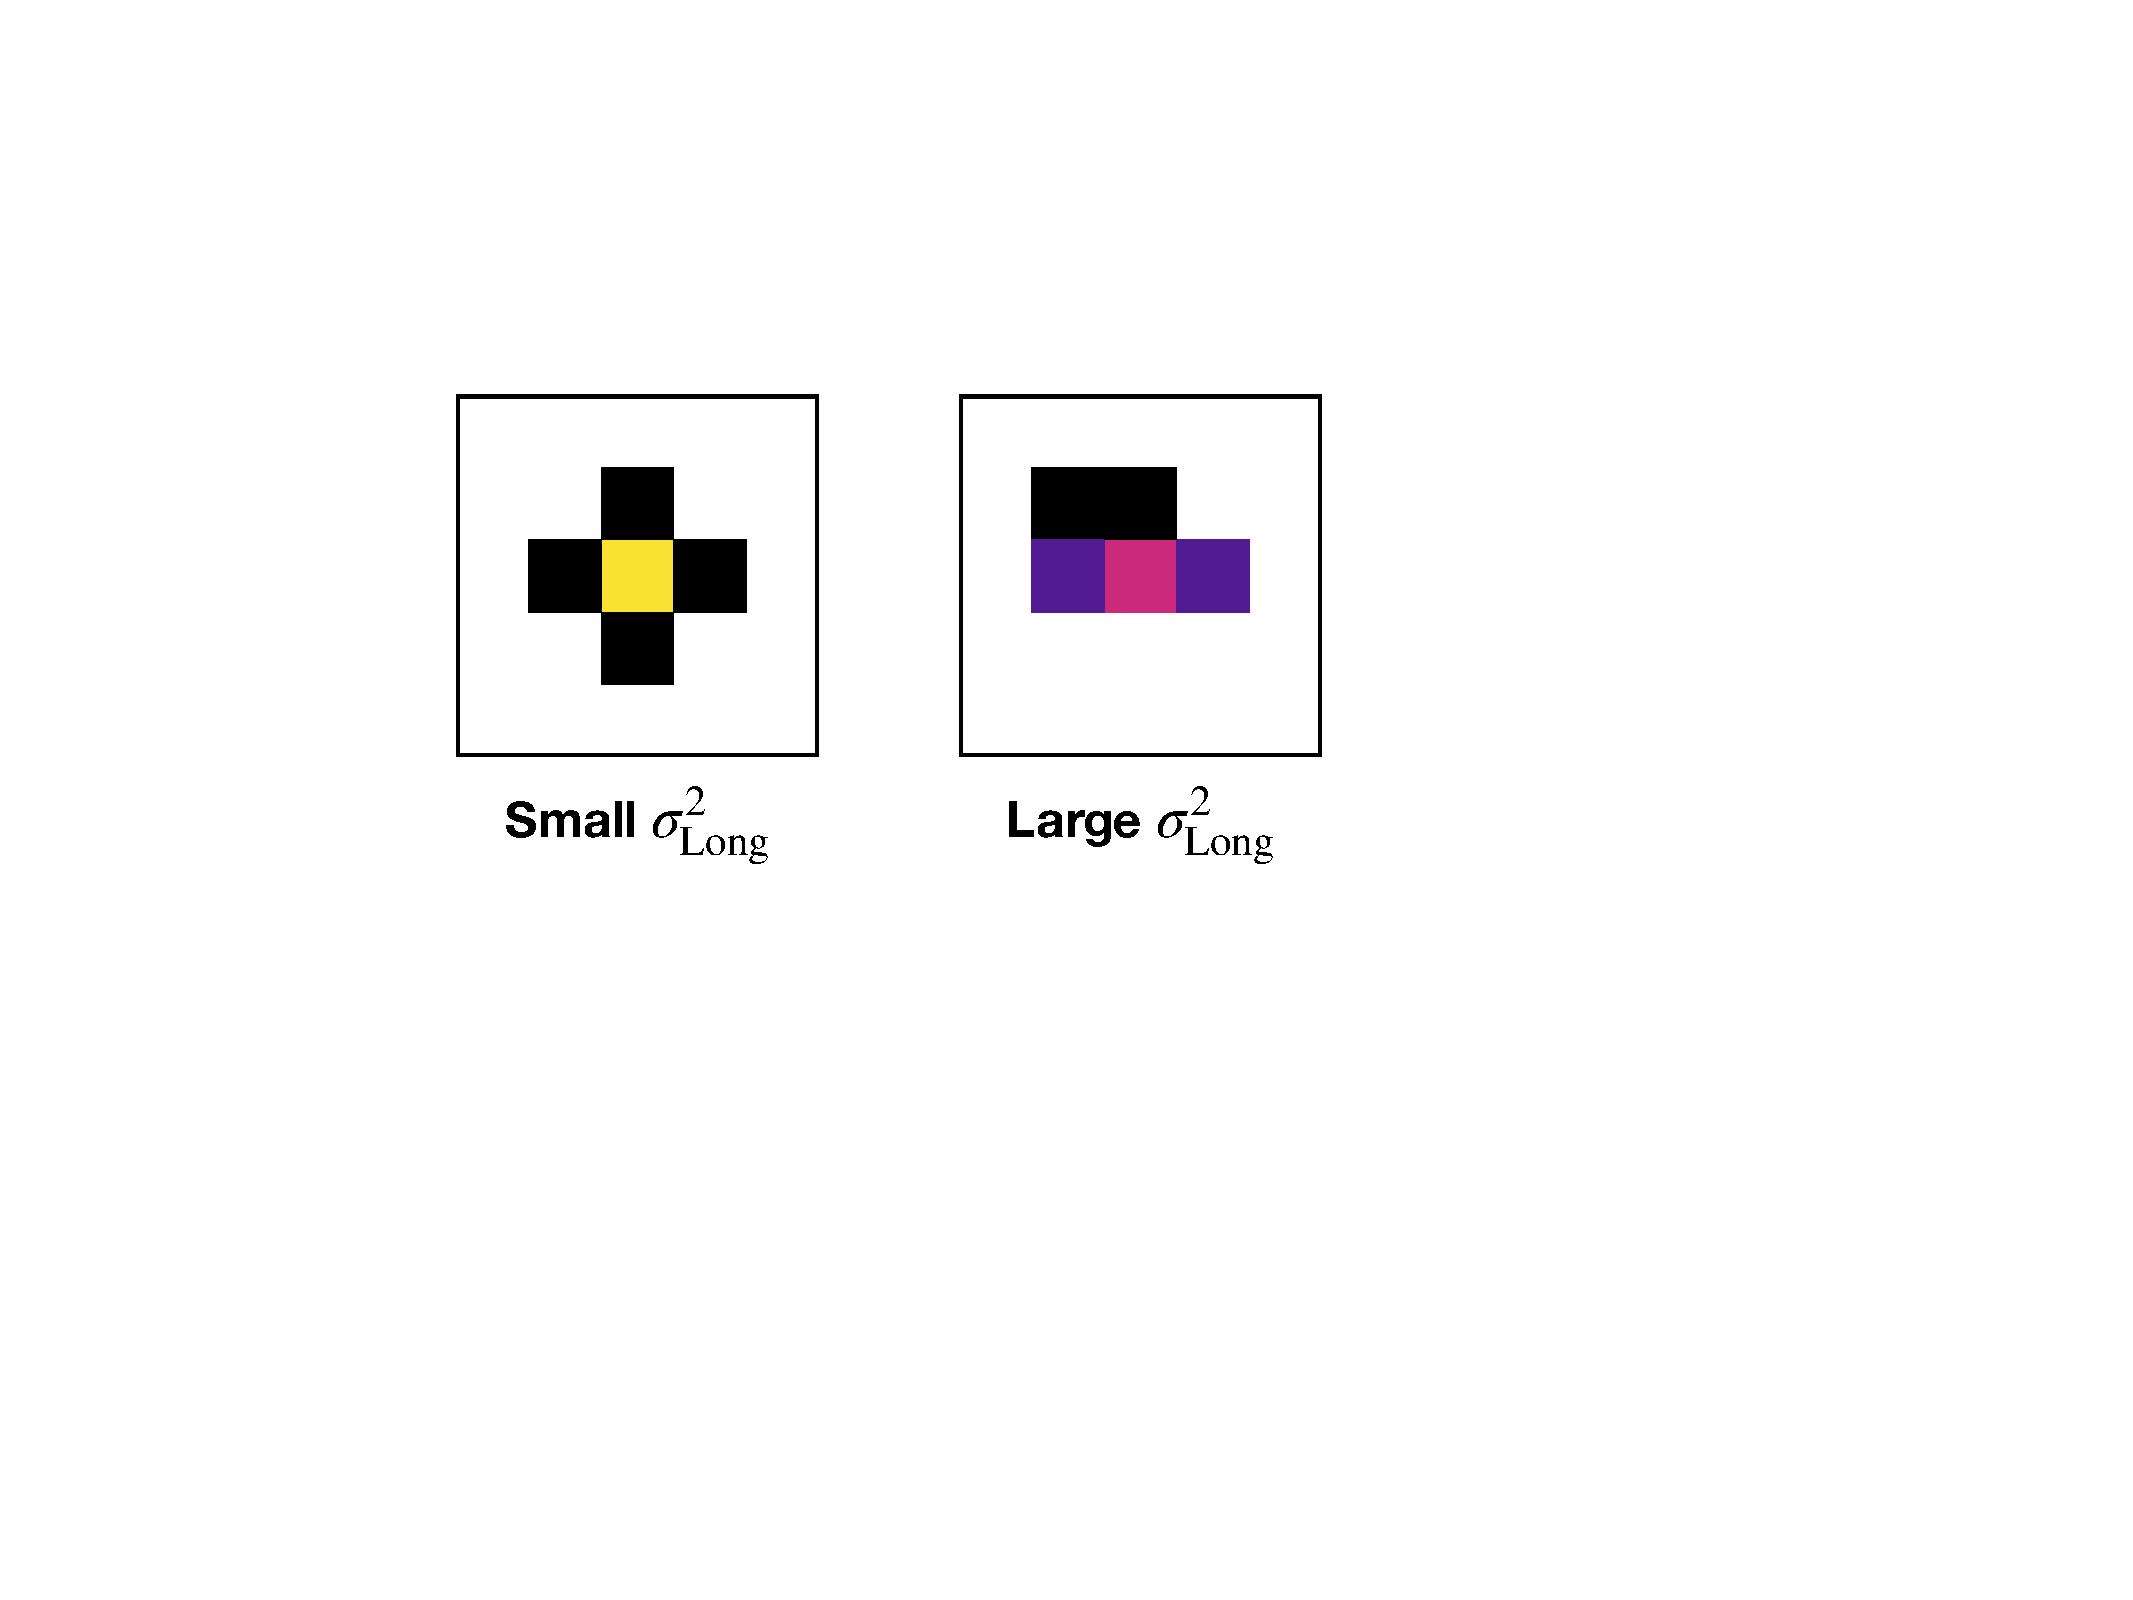
\includegraphics[width=0.5\textwidth]{Data_Analysis/sigma_long_shapes.pdf}
  \caption{Cartoon of a narrow EM shower profile with a small \lambdasquare (left), and an elongated shower profile with a larger \lambdasquare.}
  \label{fig:sigma_long_shapes}
\end{figure}

The shower shape profile is an important tool to help discriminate between clusters belonging to single photons, for which the $\lambdasquare$ distribution is narrow and symmetric, and merged photons from neutral-meson decays, for which the distribution is dominated by a long tail towards higher values. This analysis uses a cutoff of $\lambdasquare < 0.3$ to identify single photon candidates, which will be discussed in Sec.~\ref{sec:purity}.

\subsection{Photon Isolation Requirement}
\label{sec:isolation}
At leading order in pQCD, prompt photons are produced in 2$\to$2 processes surrounded by very little hadronic activity, in contrast to fragmentation photons and high \pt \pizero's found within a jet. Beyond leading order, the direct and fragmentation components cannot be factorized. As a result, the sum of their cross sections becomes the physical observable.\\

Despite this, the contribution from fragmentation photons can be suppressed by enforcing an isolation criteria, where the energy surrounding a photon must be less than a certain threshold. 
Theoretical calculations can also be simplified through the use of an isolation requirement. \cite{PhysRevD.82.014015}. This also has the benefit of suppressing the background from decays of neutral mesons often found within jets.

The simplest definition of isolation is defined as the scalar sum of the transverse momentum of charged particles within an angular radius, $R =\sqrt{(\Delta\varphi)^{2} +(\Delta\eta)^{2}  }$, around the cluster direction. This measurement uses $R = 0.4$, which is a common value used in various jet measurements.

\begin{equation}
\pt^\mathrm{iso,raw} = \sum_{\mathrm{track}~\in\Delta R<0.4} p_{\mathrm{T}}^{\mathrm{track}}	
\end{equation}

This does not, however, take into account the energy arising from the underlying event, described in the following section.
%Define underlying event


\subsection{Underlying Event Estimation for Photon Isolation}
\label{sec:ue_isolation}

The underlying event (UE) is defined as the sum of all processes that make up the final hadronic state in a collision, excluding the leading order hard scattering.When the two neuclei, lorentz contracted into discs tiny fraction of a femtometer thick, overlap or collide, a small fraction of the incident partons suffer hard perturbative interactions as the discs overlap initially. Most of the incident partons, however, lose some energy but are not deflected by any large angle. Most of these interactions are soft and involve little transverse momentum transfer. In the language of fields and particles, as the two discs of strongly interacting transverse color fields and associated color charges collide, some color charge exchange occurs between the discs, and longitudinal color fields are produced, which fill the space between the two receding discs, reducing the energy in the discs themselves, and then gradually decay into $q\bar{q}$ pairs and gluons. These processes can be labelled as multi-parton interactions, as well as both initial and final state radiation, but the term underlying event also includes measured beam fragments. Essentially, the underlying event is made up of all the particles not directly associated with the initial hard scattering of the collision.
% Sources of underlying event can include beam fragments, 

Here we describe the method used to estimate the underlying event for the purposes of correcting the isolation requirement (not to be confused with the later section \ref{sec:ue_subtraction}, where the contribution from the underlying event to the azimuthal correlation measurement is described).

We use the jet area/median method\footnote{From the \textsc{FastJet} software packace::VoronoiAreaSpec \url{http://www.fastjet.fr/repo/doxygen-2.4.5/classfastjet_1_1VoronoiAreaSpec.html} } which estimates the underlying event energy density,~$\rho$, from the median of the distribution of the transverse momentum densities of the jets in the event ~\cite{Cacciari:2009dp}. Jets are reconstructed by running the $k_\mathrm{T}$ reconstruction algorithm over all charged particles in the event, using a resolution parameter of R = 0.3. The \kt algorithm is used here in place of the more standard anti-\kt as it groups particles with the lowest momentum first to construct the jet. This makes the \kt algorithm more sensitive to the softer objects in the event, and therefore more suitable for studying the underlying event.The transverse momentum density of each jet is simply the momentum of the jet divided by its area, determined by the sum of the voronoi cells of each particle within the jet\footnote{The voronoi cell is the region for each "seed", or particle, that  consists of all points in the same  plane that are closer to that seed than to any other.}. 
 This median calculation is described in Equation \ref{eq:ue_density}:
\begin{equation}
\label{eq:ue_density}
  \rho = \mathrm{med} \left\{ \frac{\sum_{i\in J'_k}
    p_{T,i}}{\sum_{i\in J'_k} A_i} \right\}
\end{equation}
where $p_{T,i}$ is the transverse momentum, and $A_i$ the Voronoi area of the particle $i$ within the jet, $J'_k$, reconstructed for UE estimation purpose.  The median is determined from all jets in the event with the important exception of the two leading (highest moment) jets in the event, as those are most often associated with the hard scattering of the collision. This therefore assumes that most of the charged particles in the event is made up of soft particles, and that the charged particles originating from the hard scattering of the collisions are reasonably contained within the leading jets of the event ~\cite{Cacciari:2009dp}.\\

\begin{figure}
\label{fig:Rho}
	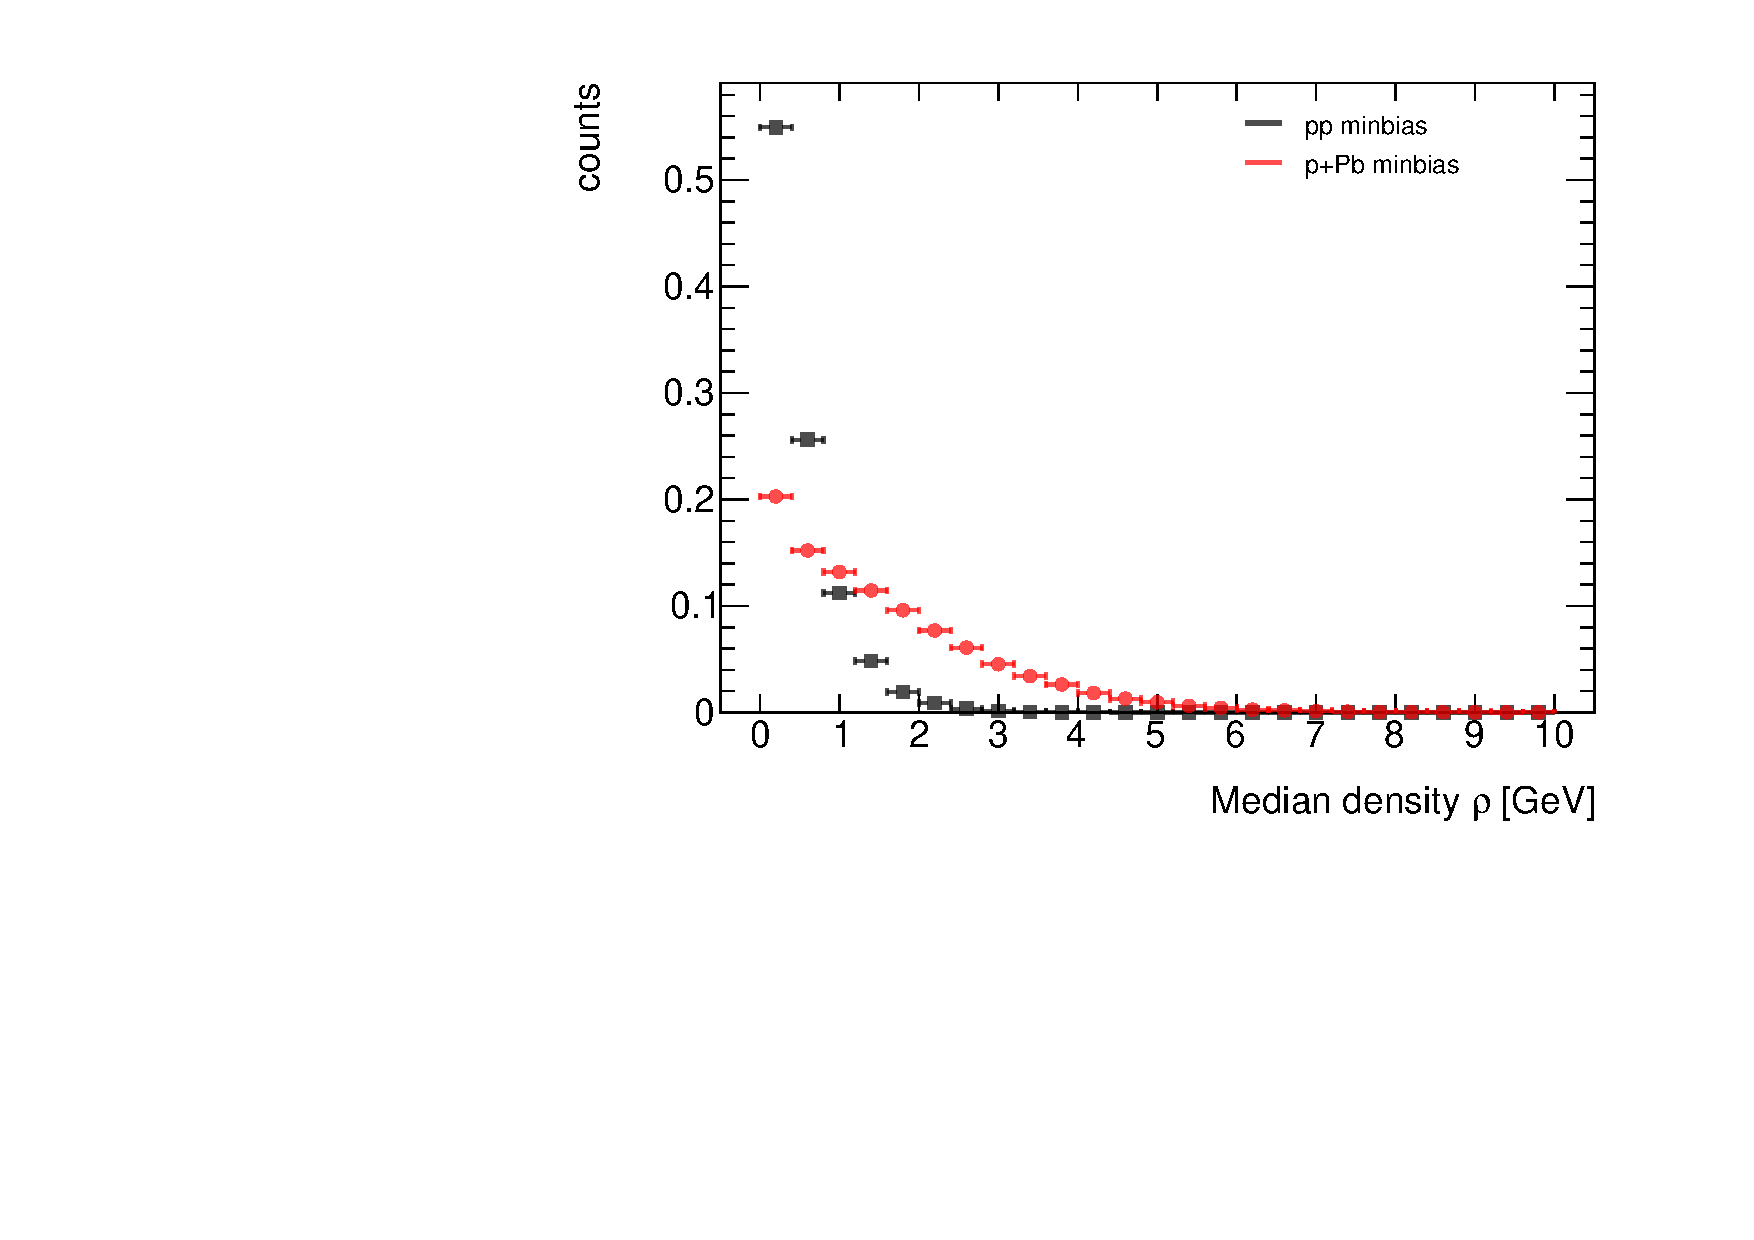
\includegraphics[width=0.5\textwidth]{Data_Analysis/Isolation/Rho_MinBias}
	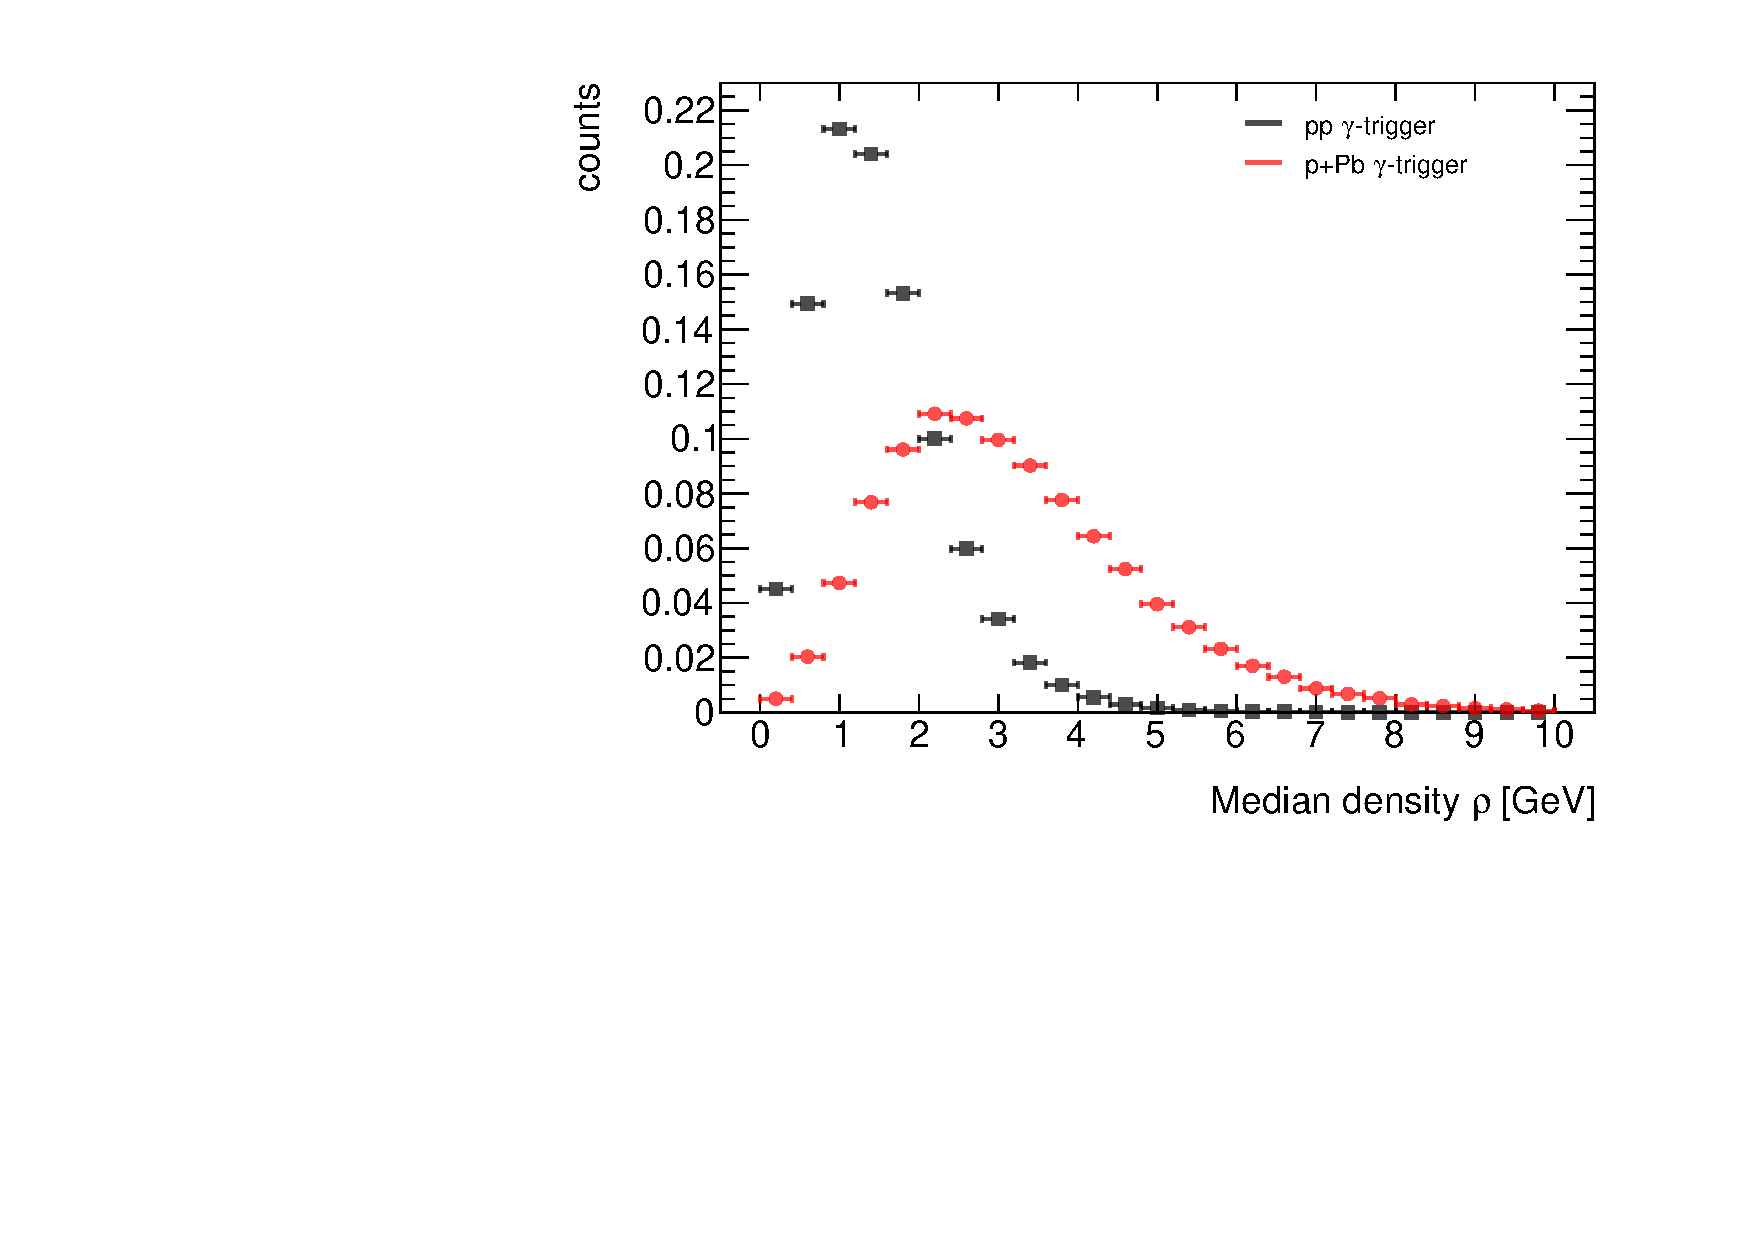
\includegraphics[width=0.5\textwidth]{Data_Analysis/Isolation/Rho_GammaTrigger}
	\caption{Distribution of the median charged-particle transverse momentum density, $\rho$, in pp and \pPb~data, for a minimum-bias selection (left panel) and in photon-triggered events (right panel).}
\end{figure}

The charged-particle density, $\rho$, is calculated for each event. Figure \ref{fig:Rho} shows the distribution of $\rho$ for minimum bias and gamma-triggered events in pp and \pPb. Average values are 3.2 \GeVc~in photon- triggered events in \pPb~and 1.6 \GeVc~in pp collisions, demonstrating the a larger underlying event activity in \pPb compared to pp.


The mean and standard deviation for each distribution is shown in Table~\ref{tab:rhoestimates}. The difference in UE-density in \pPb~is expected due to the increased number of nucleon-nucleon collisions. The UE-densities shown here are still about a factor of 50 lower than in central Pb-Pb collisions.
\begin{table}[h]
   \centering
   \caption{Median transverse momentum density mean and standard deviation in minimum-bias and and photon-triggered events in pp and \pPb~data, calculated with negligible statistical uncertainties.}
   \label{tab:rhoestimates}
   \begin{tabular*}{1.0\columnwidth}{@{\extracolsep{\fill}}lcc|cc@{}}
    \hline
     &  pp minbias & pp $\gamma-$trigger & \pPb~ minbias & \pPb~$\gamma$-trigger  \\
       \hline
       $\langle\rho\rangle$   & 0.49 \GeVc & 1.51 \GeVc & 1.56 \GeVc & 3.19 \GeVc \\ 
       $\sigma_{\rho}$       &  0.47 \GeVc &  0.85 \GeVc  & 1.32 \GeVc & 1.60 \GeVc \\ 
            \hline        
   \end{tabular*}
\end{table}

%TODO: Write about lack of neutrals in isolation
%isolation variable does not include neutral particles. This enables us to use the full acceptance of the EMCal and reduces biases arising from correlation with the opening angle of $\pi^{0}$ decays. However, it does result in a slightly lower purity of the isolated single photon signal. 

\subsection{UE Correction to Isolation Variable}
\label{sec:ue_correction_isolation}
For each cluster in the event, the underlying event is subtracted using the measured charged-particle density $\rho$ that is calculated event-by-event as described in Section~\ref{sec:ue_isolation}:

%For the determination of the isolation criterium,~$\pt^\mathrm{iso}$, the background due to the underlying event is estimated with the Voronoi method from the \textsc{FastJet} jet area/median package~\cite{Cacciari:2009dp} on an event-by-event basis and subtracted according to:

The result is an average subtraction for the isolation cone of {$R=0.4$} is about {$1.6$ \GeVc} and {$0.8$ \GeVc} for \pPb~and pp collisions, with a standard deviation of {0.9 \GeVc} and {0.4 \GeVc}, respectively.  

%A requirement of $\pt^\mathrm{iso}<1.5$ \GeVc is used, which results in a signal efficiency of about 90$\%$ that does not significantly depend on the photon $\pt$. 
 
For photons near the edge of the detector, the isolation energy requirement is scaled to account for any missing area in the isolation cone\footnote{The final isolated photon-hadron correlations are normalized to the number of reconstructed photons. As a result, the $\gammaiso$ efficiency was not studied in detail.}. A check on on this scaling procedure was also done in Section \ref{sec:iso_acceptance_check}. 
\begin{equation}
p_T^\mathrm{iso} = p_T^\mathrm{iso,raw} - \rho\times\pi(0.4)^{2}.
\end{equation}

Figure~\ref{fig:iso_ue} shows the isolation distribution before and after underlying event subtraction for \pPb~and pp collisions. The distributions have a positive tail that decreases exponentially. This is likely due to the sensitivity of the isolation variable on multi-jet production cross section. The difference between the \pPb~and pp distribution at low $\ptiso$ values can be attributed to the effect of enhanced soft-particle production in \pPb~collisions, i.e. a larger underlying event due to the presence of the pPb nucleus. The underlying event subtraction modifies the isolation distribution only slightly at high \pt. At low and negetaive \pt, however, the distributions show a negative tail after subtraction, which arises from an over-subtraction of the underlying event. This occurs due to region-to-region fluctuations in the underlying event, where a cluster contains an energy density that is smaller than the median calculated according to Section \ref{sec:ue_isolation}. In both cases, this tail falls by more than three orders of magnitude by $\ptiso=-3$ \GeVc, indicating that over-subtraction is a small effect.   

\begin{figure}[h]
\center
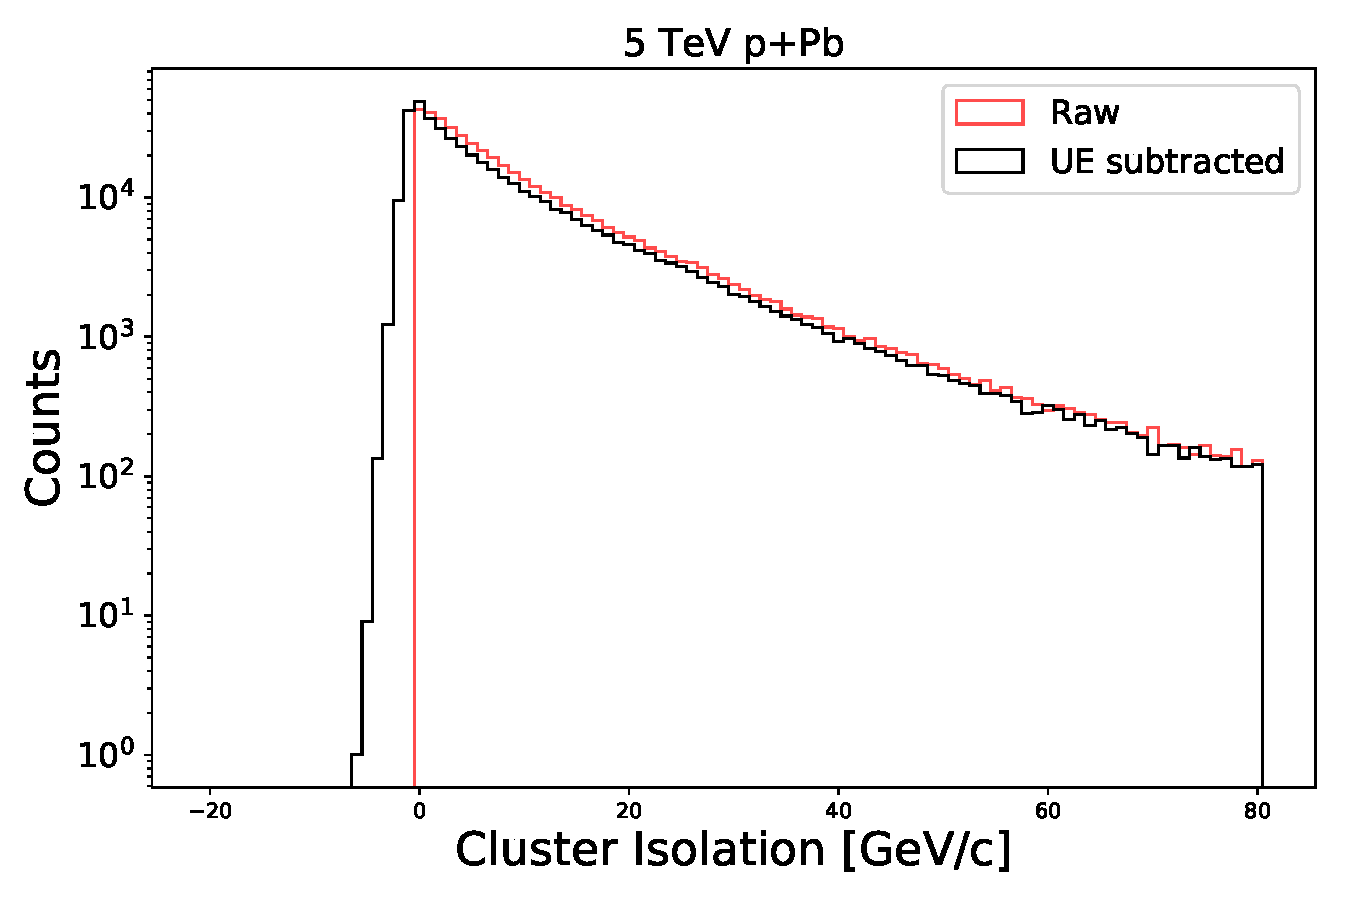
\includegraphics[width=0.49\textwidth]{Data_Analysis/Isolation/IsolationWithUESubtraction_Skimmed_13def_root}
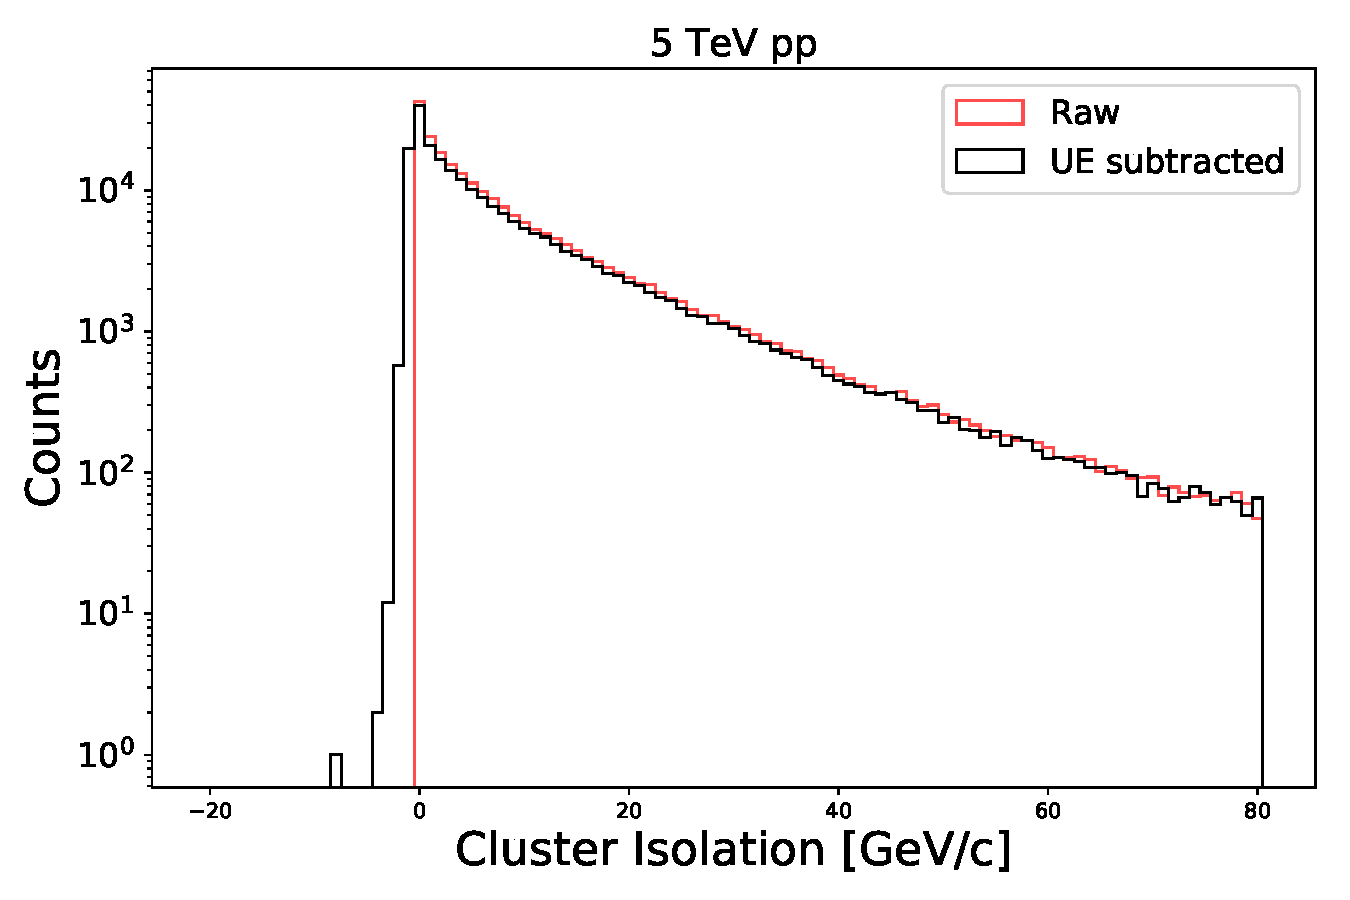
\includegraphics[width=0.49\textwidth]{Data_Analysis/Isolation/IsolationWithUESubtraction_Skimmed_17q_root}
\caption{Cluster isolation before and after underlying event subtraction in \pPb~(left panel) and pp (right panel) collisions.}
\label{fig:iso_ue}
\end{figure}

%TODO Fix Table Reference
The left panel of Figure~\ref{MC_Isolation} shows the distribution of cluster isolation after UE subtraction for photon-jet and dijet simulations of \pPb~data (see Table~\ref{tab:MCsamples}). The distributions exhibit different behavior: whereas the dijet simulation shows a prominent exponential tail at large $\ptiso$ values, the photon-jet simulation shows a more Gaussian-like shape that is mostly symmetric with the exception of a very small fraction of events that have large $\ptiso$ values. In both cases, however, the negative tail falls rather sharply, as it arises from region-to-region fluctuations of the UE that are independent of the hard-process involved. 

\begin{figure}[h]
\center
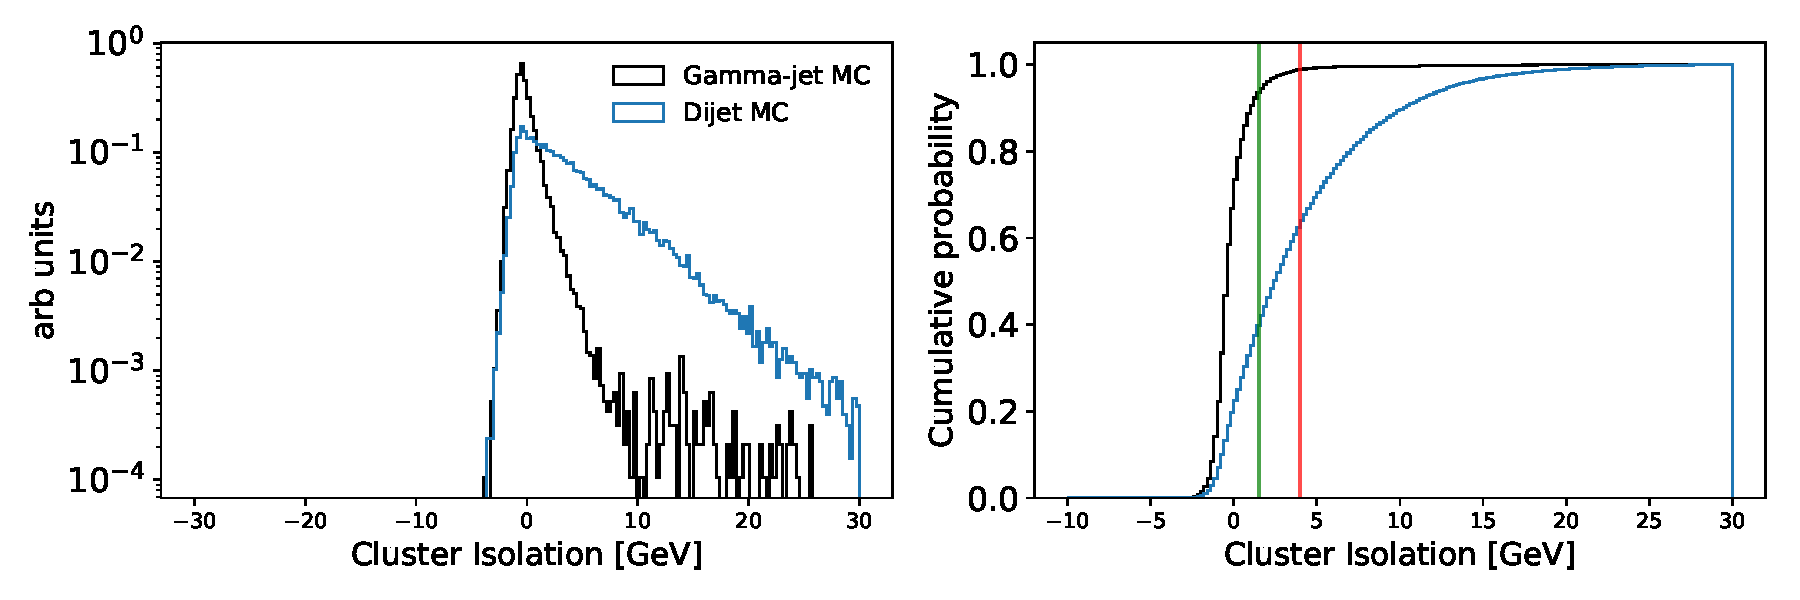
\includegraphics[width=1.0\textwidth]{Data_Analysis/Isolation/IsolationMCsignal_Skimmed_17g6a1_pthat1_4L_root}
\caption{Isolation distribution of clusters that pass our selection in \pPb~photon-jet and dijet simulations, and corresponding cumulative distribution. Two vertical lines at $\ptiso=$ 1.5 \GeVc~(green) and $\ptiso=$ 5.0 \GeVc~are shown in the right panel for reference.}
\label{MC_Isolation}
\end{figure}

%For the purposes of template fitting, we also need to define a sideband that is dominated by background. For this we note that only about 1$\%$ of prompt photons of the photon-jet simulation have {$\iso>$ 5 \GeVc}. Given that the cross-section for prompt photons is about two orders of magnitude smaller than the background, this region is overwhelmingly dominated by background.   

The cumulative distributions (Figure~\ref{MC_Isolation}, right panel) show that a {$\ptiso<$ 1.5 \GeVc} selection keeps about 90$\%$ of the signal and rejects about 60$\%$ of the background. This relatively loose photon isolation criteria is used in order to reduce the dependence of the results on the details of the simulation of the detector noise, tracking resolution, and the underlying event. 


\subsection{Remaining Background after Photon Selection}

This isolation cut of {$\ptiso<$ 1.5 \GeVc} is used in conjunction with the shower-shape cut  of $0<\lambdasquare<0.3$ to complete the isolated-photon selection or ``$\gammaiso$ selection''. The population of clusters that pass this selection are labelled``$\gammaiso$-candidates'' (rather than simply ''prompt photons'') because there is still a significant fraction of remaining background. Some other sources of background not yet mentioned arise from charged-to-neutral fluctuations of jet fragmentation that leads to low observable $\ptiso$ (that considers only charged-particles). However, the main background present in the $\gammaiso$ selection arise from multi-jet events where one jet typically contains a $\pi^{0}$ or $\eta$ which carries most of the jet energy, and is therefore surrounded by relatively less energy within the jet. The pair is also frequently misidentified as a single photon because it decays into a pair of photons that are collinear with respect to the EMCal cell granularity. The first indication of this is shown in Figure \ref{MC_Isolation}, where approximately 40\% of the dijet cross section (expressed as a cumulative probability as a function of cluster isolation, shown in blue) is within $\ptiso < 1.5 \GeVc$.\\ Distributions of background and signal as function of \lambdasquare are shown later in \ref{sec:purity}

Figure \ref{fig:cross_section_camparison} expands on this. The left panel shows the isolated photon differential cross section as a function of \ptgamma in proton-proton collisions at \sqrts = 5.02 TeV measured by the ALICE detector. The right panel of Figure shows the differential cross section of charged jets as a function of $\pt^\mathrm{jet}$. The cross section for an isolated photon at \pt = 20 \GeVc~is roughly 2nb $\GeVc^{-1}$. In contrast, the cross section for charged jets at \pt = 20 \GeVc~is roughly 2$\times10^{-3}$mb $\GeVc^{-1}$, approximately three orders of magnitude larger. 

\begin{figure}
\centering
	\label{fig:cross_section_camparison}
\raisebox{0.9cm}{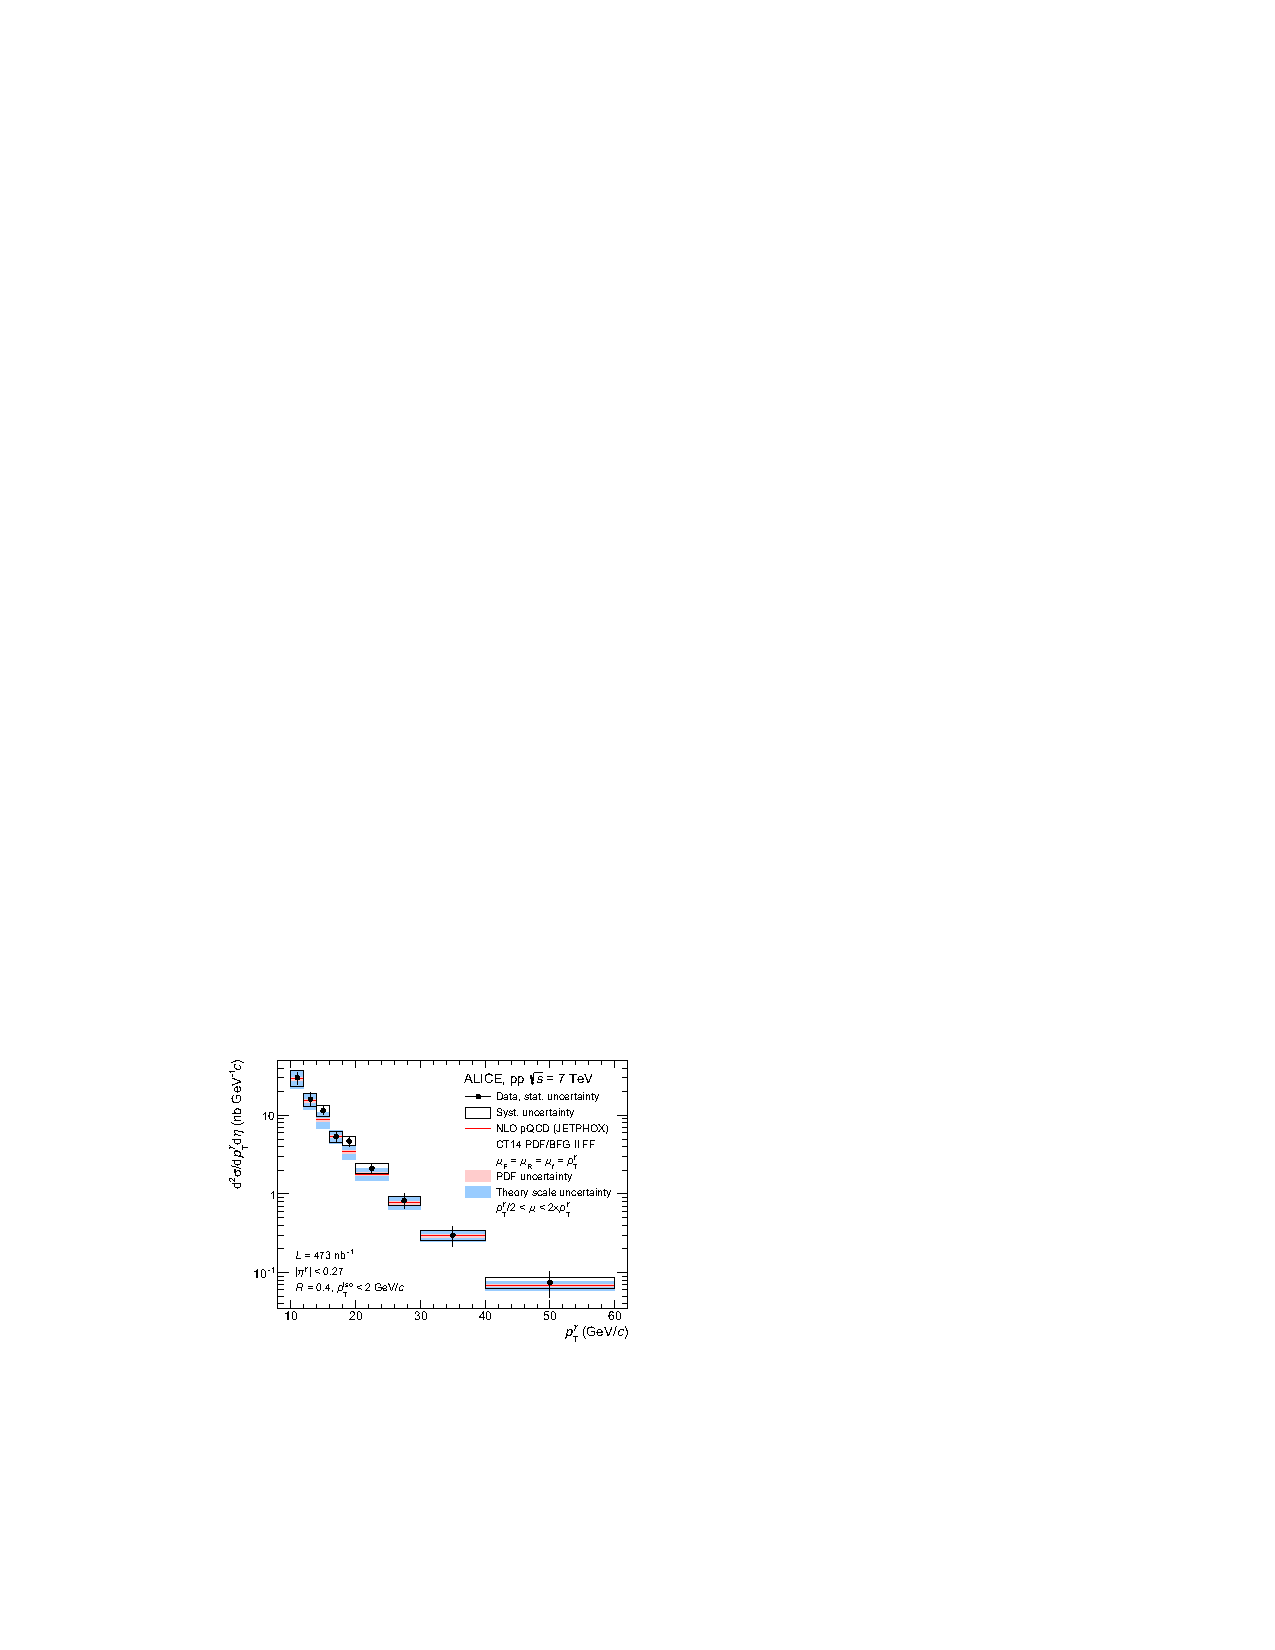
\includegraphics{Data_Analysis/Isolation/isolated_photon_cross_section}}
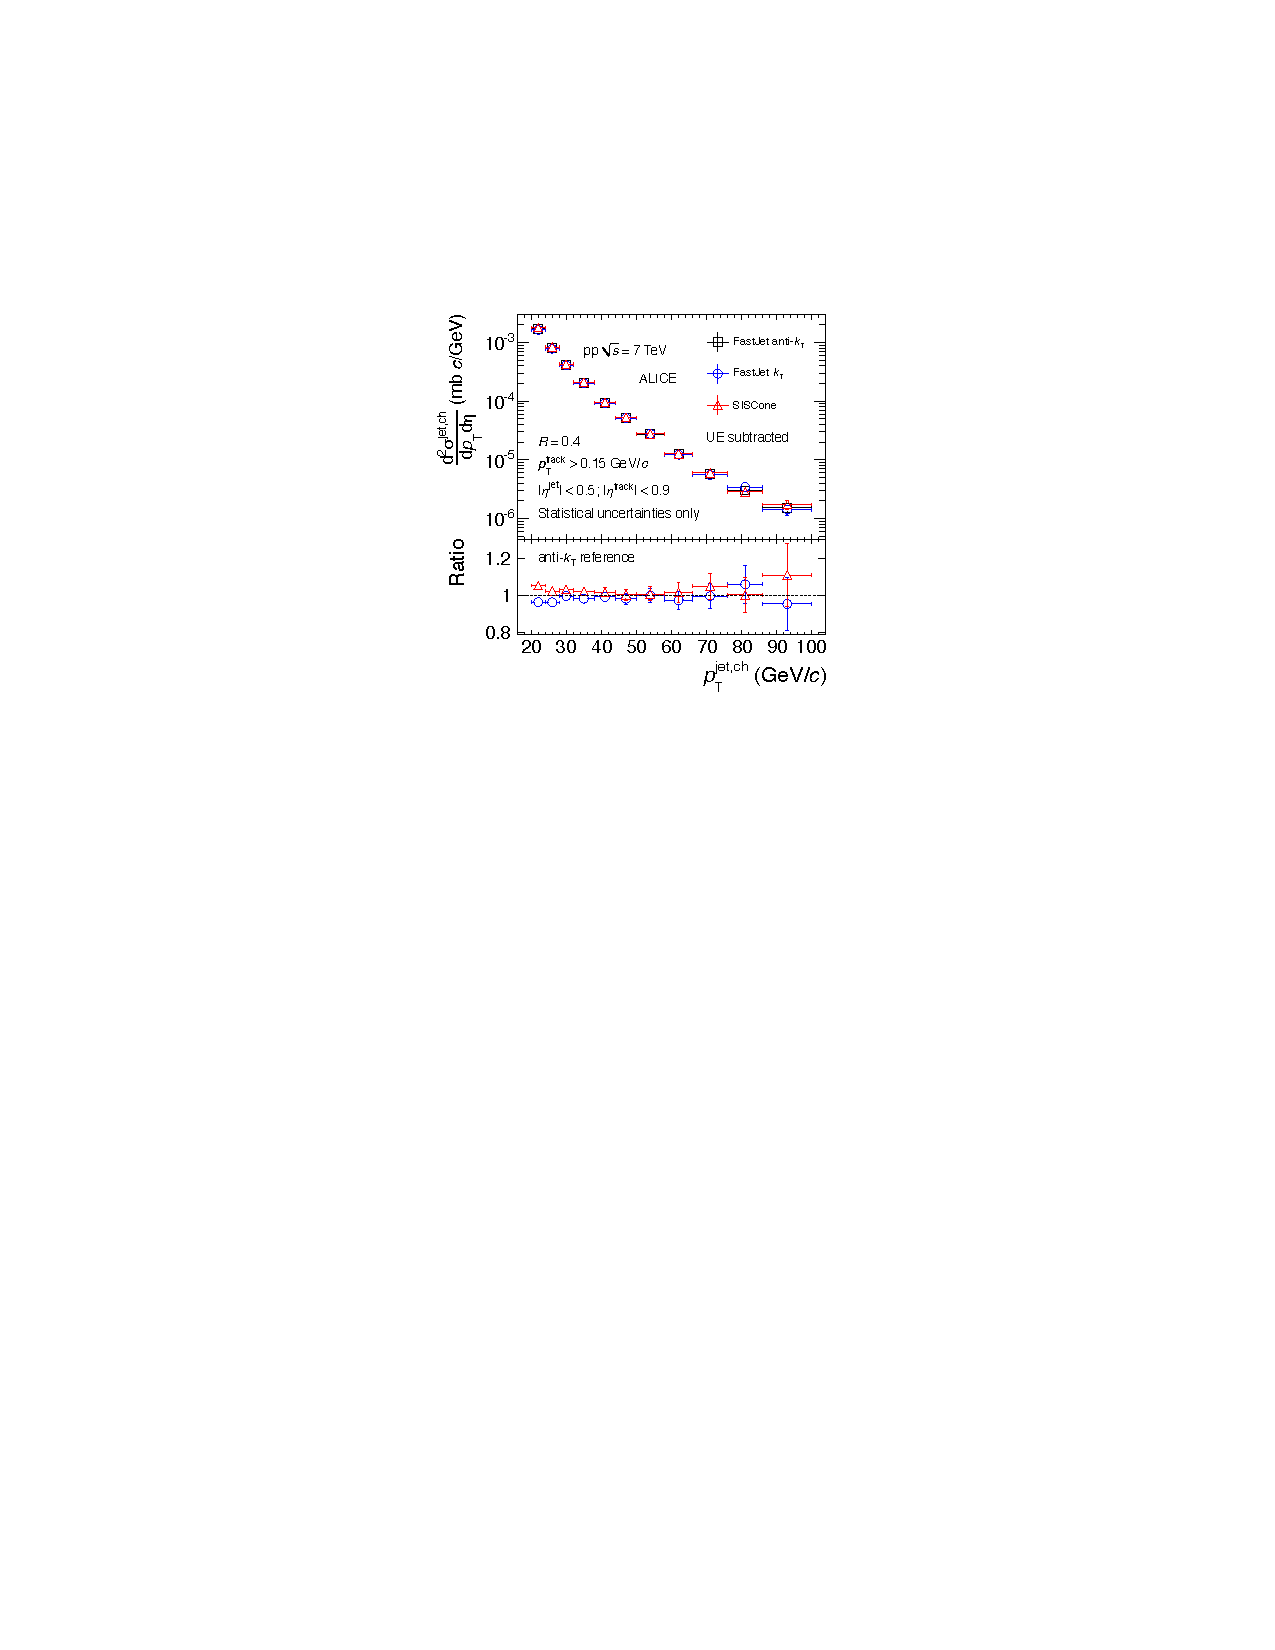
\includegraphics{Data_Analysis/Isolation/charged_jet_cross_section}
\end{figure}

 

Of course, jets containing a neutral meson with a large fraction of its total momentum make up only a fraction of the total jet cross section, and recoil partons produced from the same hard scattering as prompt photons will contribute to the total charged jet cross section. But the stark difference between the isolated photon and charged jet cross sections speaks to the rarity of isolated photons in these collisions and the abundance of background and illustrates the need to measure the purity of our $\gammaiso$-candidate selection.%, which is described in Section~\ref{sec:purity}. 

%r



%A \pizero with sufficiently high \pt, approximately 6~\GeVc, a \pizero will decay into two photons with such a small opening angle, that their electromagnetic showers from the two photons in the ALICE EMCal significantly overlap. %significantly overlapping elecromagnetic showers in the calorimeter
%For this reason, the two showers from the two photons will appear in the ALICE EMCal as a single cluster.

%Thus, in order to select against this measurement's largest source of background, we require that clusters have a more symmetric shape in the EMCal.
\section{Purity}
\label{sec:purity}
The isolation and shower shape selections remove the bulk of the neutral meson decay background, but a substantial fraction of the \gammaiso candidates are still background photons. It is therefore necessary to quantify the ratio of true signal photons in our candidate sample in order properly subtract it. The estimate of the ratio of true signal photons in our \gammaiso sample is called the \textit{purity}. \footnote{For a more rigorous discussion of the Purity calculation, please see Alwina Liu's UC Berkeley Thesis.}

\subsection{The Template Fit Method}
The purity of the isolated photon sample is determined with a two-component template fit, a method used by the CMS collaboration in Ref.~\cite{Sirunyan:2017qhf}. The distribution of the shower shape variable for the isolated cluster sample is fit to a linear combination of a signal distribution and the background distribution. The shape of the signal distribution is determined by a photon-jet simulation (see Table~\ref{tab:MCsamples}) and the shape of the background distribution is determined from data using an anti-isolated sideband~\footnote{The inversion of an isolation cut to estimate QCD background is a standard technique in several measurements at the LHC and previous hadron colliders.} with an additional correction computed from a dijet simulation. This is described in more detail in the following sections.  

\subsection{Signal Template and Background Templates }
The shape of the background distribution of the shower-shape for isolated clusters is estimated with a \textit{sideband} technique: the shower shape distribution of clusters from isolated decay photons is estimated with clusters that are anti-isolated but pass all other selection criteria. This method assumes that the correlation between the isolation variable and shower shape variable can be corrected for; the procedure for doing so is described below. The signal and sideband regions defined using the isolation variable are illustrated in Figure~\ref{SidebandDefinition}. 

\begin{figure}[h]
\center
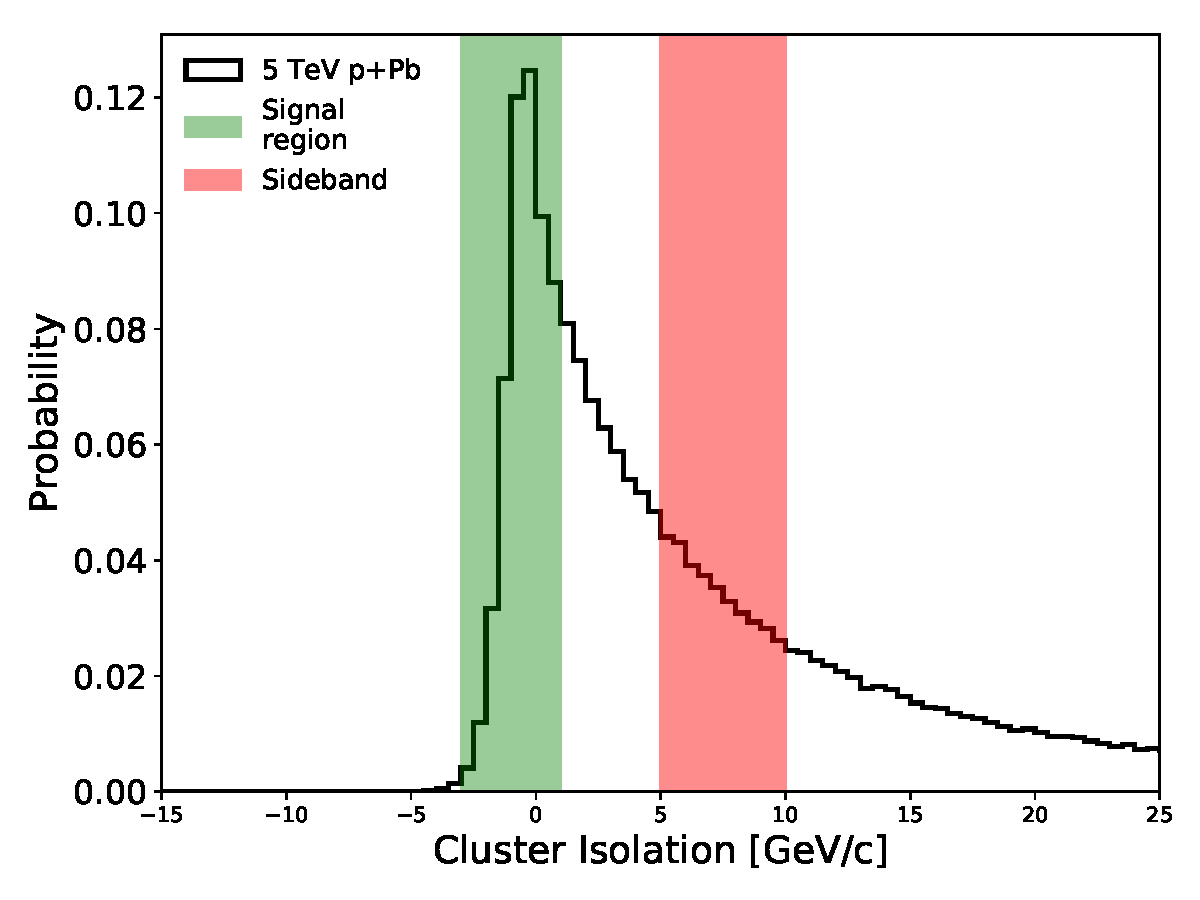
\includegraphics[width=0.49\textwidth]{Data_Analysis/Purity/IsolationSideband_limited_Skimmed_13def_root}
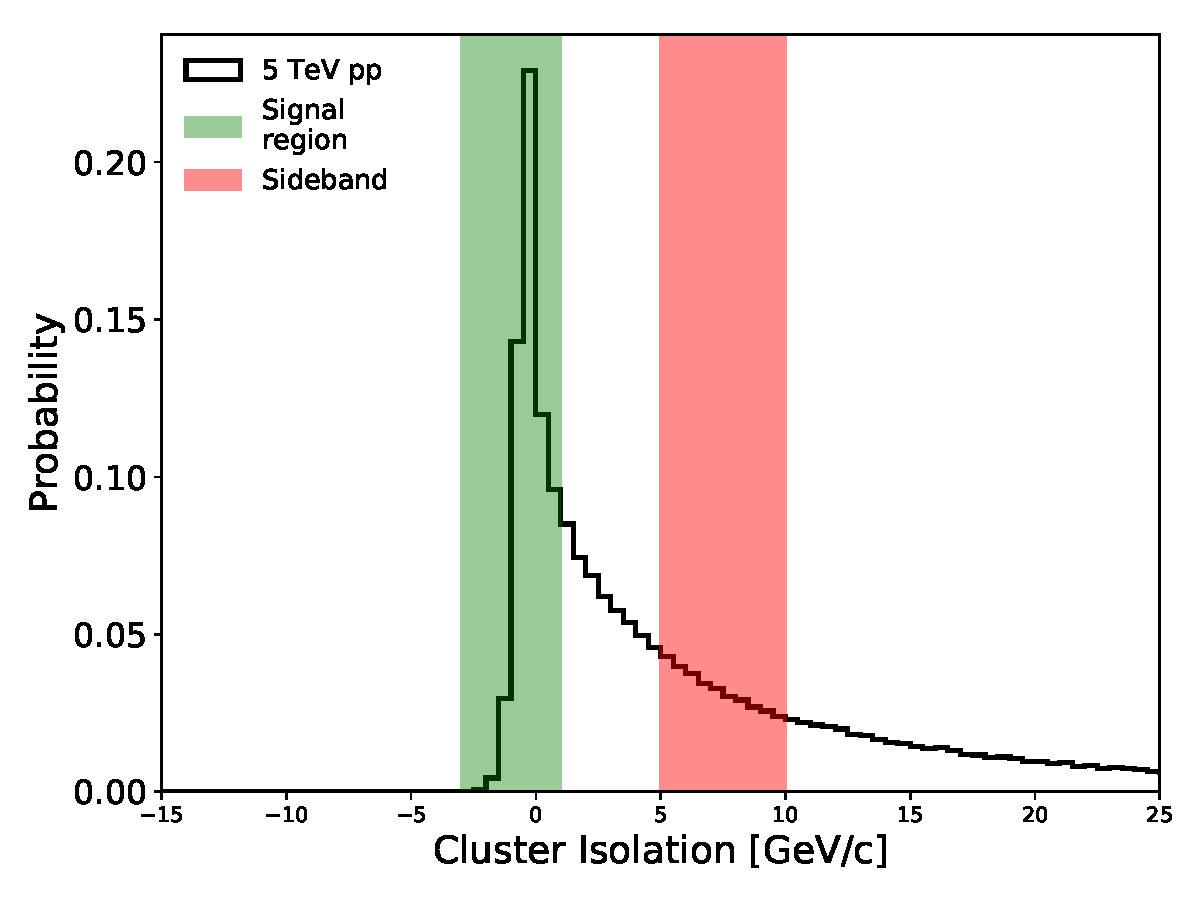
\includegraphics[width=0.49\textwidth]{Data_Analysis/Purity/IsolationSideband_limited_Skimmed_17q_root}
\caption{Isolation variable distribution of clusters with $\pt$ between 12 and 16 \GeVc~in \pPb~data (left panel) and pp data (right panel). The green shaded are represents the signal region ($\iso<$ 1.5 \GeVc); the red represent the sideband ($5<\iso<10$ \GeVc) used to estimate the background template.}
\label{SidebandDefinition}
\end{figure}

For simplicity, the same definitions are used for pp and \pPb~data. The lower bound of the sideband region is defined as {$\iso=5$ \GeVc}; according to photon-jet simulations, less than 1$\%$ of prompt photons are beyond this range. The upper bound is chosen such that the sideband is as narrow as possible, to minimize a possible bias to the shower-shape distribution due to a positive correlation with ISO, while still containing a number of clusters comparable to the signal region. A more rigorous study on the sensitivity of our purity estimate on the choice of sideband region is shown in Section~\ref{sec:bkgtemplate}.

Figure~\ref{TemplateShapes} summarizes the signal and background templates used in the template fit. The distributions are quite different, which is key for the stability of the template fit. The background shape in the $\lambdasquare$ variable shows a peak in the single-shower region but a ``bump'' that reflects a $\pi^{0}$ peak. In both cases, the peaks in the single-shower region that are observed in the background templates come mostly from collinear $\pi^{0}\to\gamma\gamma$ decays.

\begin{figure}
\center
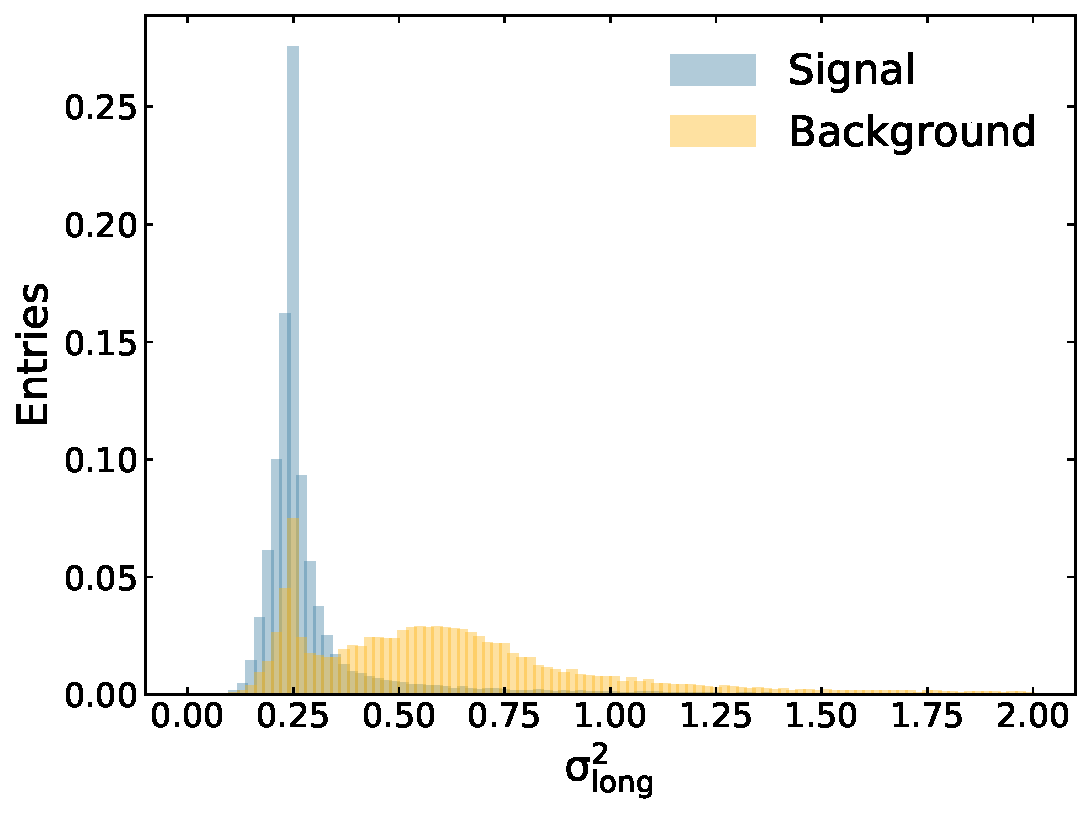
\includegraphics[width=0.5\textheight]{Data_Analysis/Purity/norm-templates-p-Pb-cluster_Lambda-15-20.pdf}
\caption{Normalized signal (blue) and background (yellow) distributions used as input for the template fit. These distributions correspond to clusters with \pt~in the 15--20 \GeVc~range.}
\label{TemplateShapes}
\end{figure}


The background template is corrected for a bias due to correlations between the shower-shape and isolation variables \cite{Khachatryan:2010fm}. 
%bvj In particular, the 
This correlation leads to clusters in the isolation sideband having a somewhat higher hadronic activity than the true isolated background. Consequently, a background template constructed from this sideband region has an increased number of background-like clusters and
%bvj which enhances the background-like region of the shower-shape distribution. This implies that the 
purity values obtained using this
 systematically overestimate the true purity.
A correction for this bias, $R(\lambdasquare)$, is determined using dijet simulated events which also contain the correlation between trigger photon shower-shape and isolation cut.
The ratio of the shower-shape distributions of clusters in the signal (Iso, $\pt^\mathrm{iso} < 1.5$ \GeVc) region and sideband (Anti-iso, $5.0 < \pt^\mathrm{iso} < 10.0$ \GeVc) region is constructed via

%The ratio of the shower-shape distributions of clusters in the signal (Iso) region and sideband (Anti-iso) region is constructed via

\begin{equation}
    R(\lambdasquare)=\frac{\text{Iso}_{\text{MC}}(\lambdasquare)}{\text{Anti-iso}_{\text{MC}}(\lambdasquare).}
    \label{eq:bkgtemplateweights}
\end{equation}
%{\color{red}  I think that a referee and our collaborators will want to know what was chosen for the sideband region. So, I suggest we just stick in the information from the start.}
This ratio of shower shape distributions is applied as a multiplicative correction to the background template:

\begin{equation}
    B^{\text{corr.}}(\lambdasquare)=\text{Anti-iso}_{\text{data}}(\lambdasquare)\times R(\lambdasquare).
    \label{eq:bkgtemplatecorrection}
\end{equation}

This background template correction results in an absolute correction on the purity of 8$\%$--14$\%$ depending on the cluster $\pt$. An example of a fit with and without the correction is shown in Figure~\ref{fig:purcorrectionexample}. The correction greatly improves the fit. 


% The purities as a function of the cluster $\pt$ are shown in Figure~\ref{fig:Purity}. 
% The background template is corrected for the correlation between the shower shape  variable and the isolation energy of the cluster. A dijet simulation is used to construct the ratio of the shower shape distribution for isolated clusters to the shower shape distribution for anti-isolated clusters. This ratio, calculated as a function of the shower shape variable, is then applied as a weight to the anti-isolated clusters in the data, giving a corrected background template that is then used in the template fit. From Equ.~\ref{eq:bkgtemplatecorrection}), it is clear that if the monte-carlo exactly replicates the data, the Weights function will exactly correct the anti-isolated decay photon \lambdasquare distribution back to the isolated decay photon \lambdasquare~distribution, which is the true background.\\ 

% \begin{align}
%     \text{Weights}(\lambdasquare)&=\frac{\text{Iso}_{\text{MC}}(\lambdasquare)}{\text{Anti-iso}_{\text{MC}}(\lambdasquare)} \nonumber \\
%     \text{Bkg}^{\text{corrected}}(\lambdasquare)&=\text{Non-iso}_{\text{data}}(\lambdasquare)\times\text{Weights}(\lambdasquare)
%     \label{eq:bkgtemplatecorrection}
% \end{align}

% The purity computed with the corrected background template is 8--13\% (absolute) lower in compared to the purity computed with the uncorrected background template; 

\begin{figure}
    \centering
    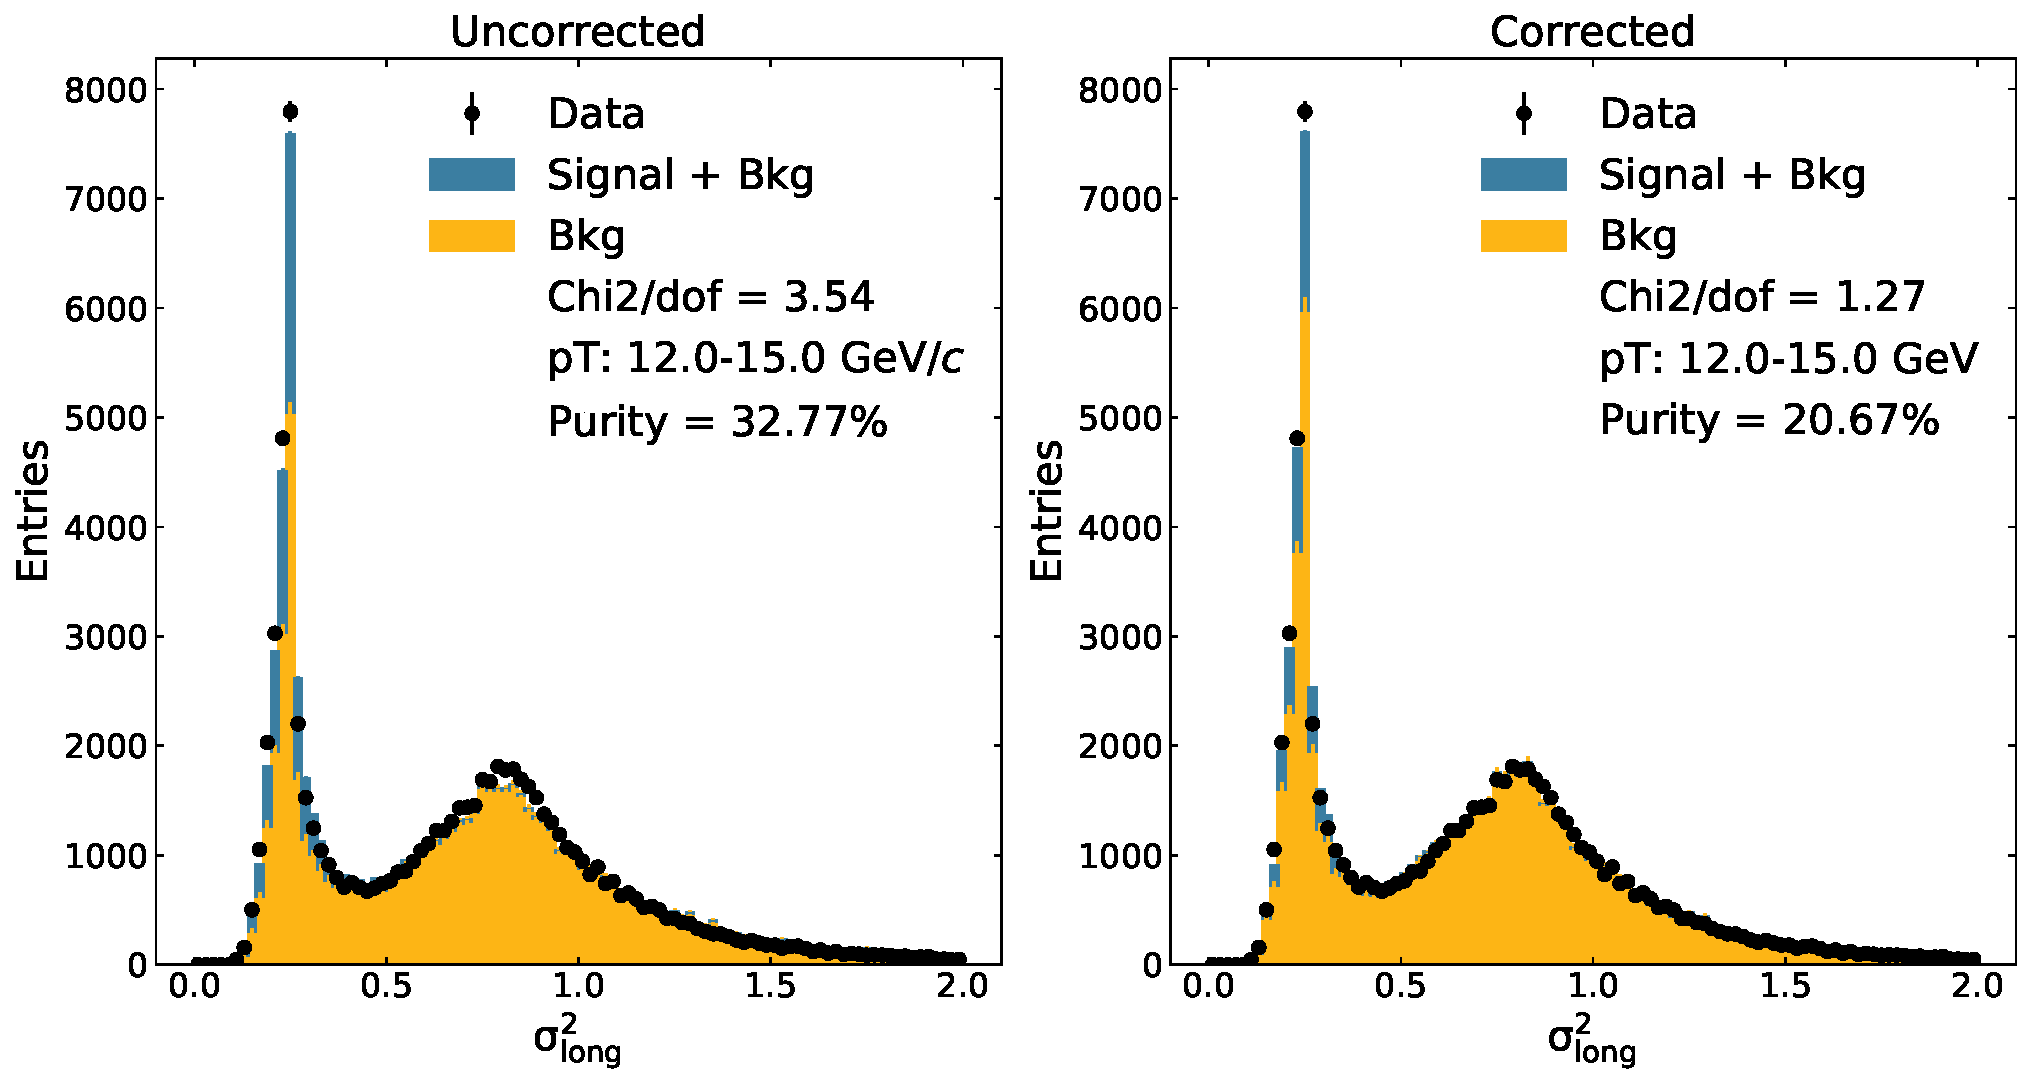
\includegraphics[width=0.5\textheight]{Data_Analysis/Purity/correction-example-p-Pb-cluster_Lambda-12-15.pdf}
    \caption{An example of the template fit with and without the background template correction in \pPb~for clusters with $12 < \pt < 15$ GeV/$c$. The goodness of fit is better after the correction and the purity is significantly lower.}
    \label{fig:purcorrectionexample}
\end{figure}
\FloatBarrier

\subsection{Fit Results}
\label{sec:fitresults}
% The \textsc{MINUIT}~\cite{James:1975dr} package is used for $\chi^{2}$ minimization and the \textsc{MIGRAD} package for error estimation. The only free parameter in the fit is the number of signal clusters, $N_{\mathrm{sig}}$, because the overall normalization, $N$, is fixed to the total number of isolated clusters:
% \begin{equation}
% N^{\mathrm{observed}} = N_{\mathrm{sig}}\times S + (N-N_{\mathrm{sig}})\times B,
% \end{equation}
% where $S$ and $B$ are the normalized signal template and background template. 


% Figures~\ref{TemplatefitResults_Preliminary} show template fit results for \pPb~and pp data. In all cases a good fit with no obvious systematic pattern in the residuals is achieved over most of the distribution, and the reduced $\chi^{2}$ ranges are within acceptable values. The purity measurements are presented in graphical form in Figure~\ref{fig:purityresults}. 
The distribution of isolated clusters is fit with a linear combination of the signal and background templates. The \textsc{MINUIT}~\cite{James:1975dr} package is used for $\chi^{2}$ minimization and the \textsc{MIGRAD} package for uncertainty estimation. The only free parameter in the fit is the number of signal clusters, $N_{\mathrm{sig}}$, because the overall normalization, $N$, is fixed to the total number of isolated clusters:
\begin{equation}
N^{\mathrm{observed}}(\lambdasquare) = N_{\mathrm{sig}}\times S(\lambdasquare) + (N-N_{\mathrm{sig}})\times B(\lambdasquare),
\end{equation}
where $S(\lambdasquare)$ and $B(\lambdasquare)$ are the normalized signal and background templates. Examples of template fits are shown in Figure~\ref{fig:TemplateFit}.
The peaks observed in the background templates originate mostly from collinear or very asymmetric $\pi^{0}\to\gamma\gamma$ decays. Photons from $\eta$ decays also contribute to the peaks in the background template.


\begin{figure}[h]
\center
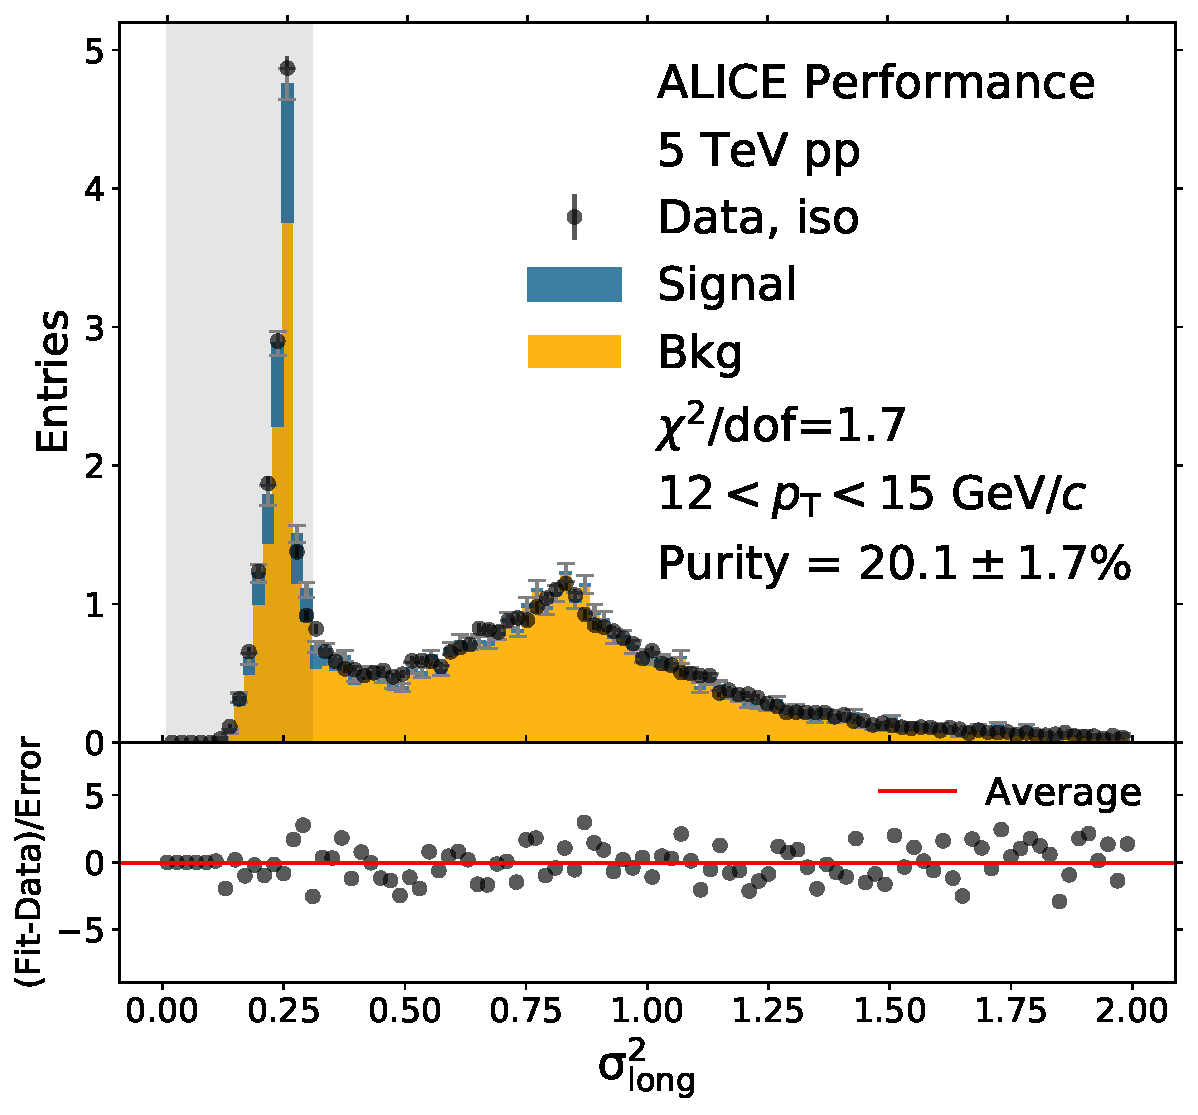
\includegraphics[width=0.3\textwidth]{Data_Analysis/Purity/tf-example-pp-cluster_Lambda-12-15.pdf}
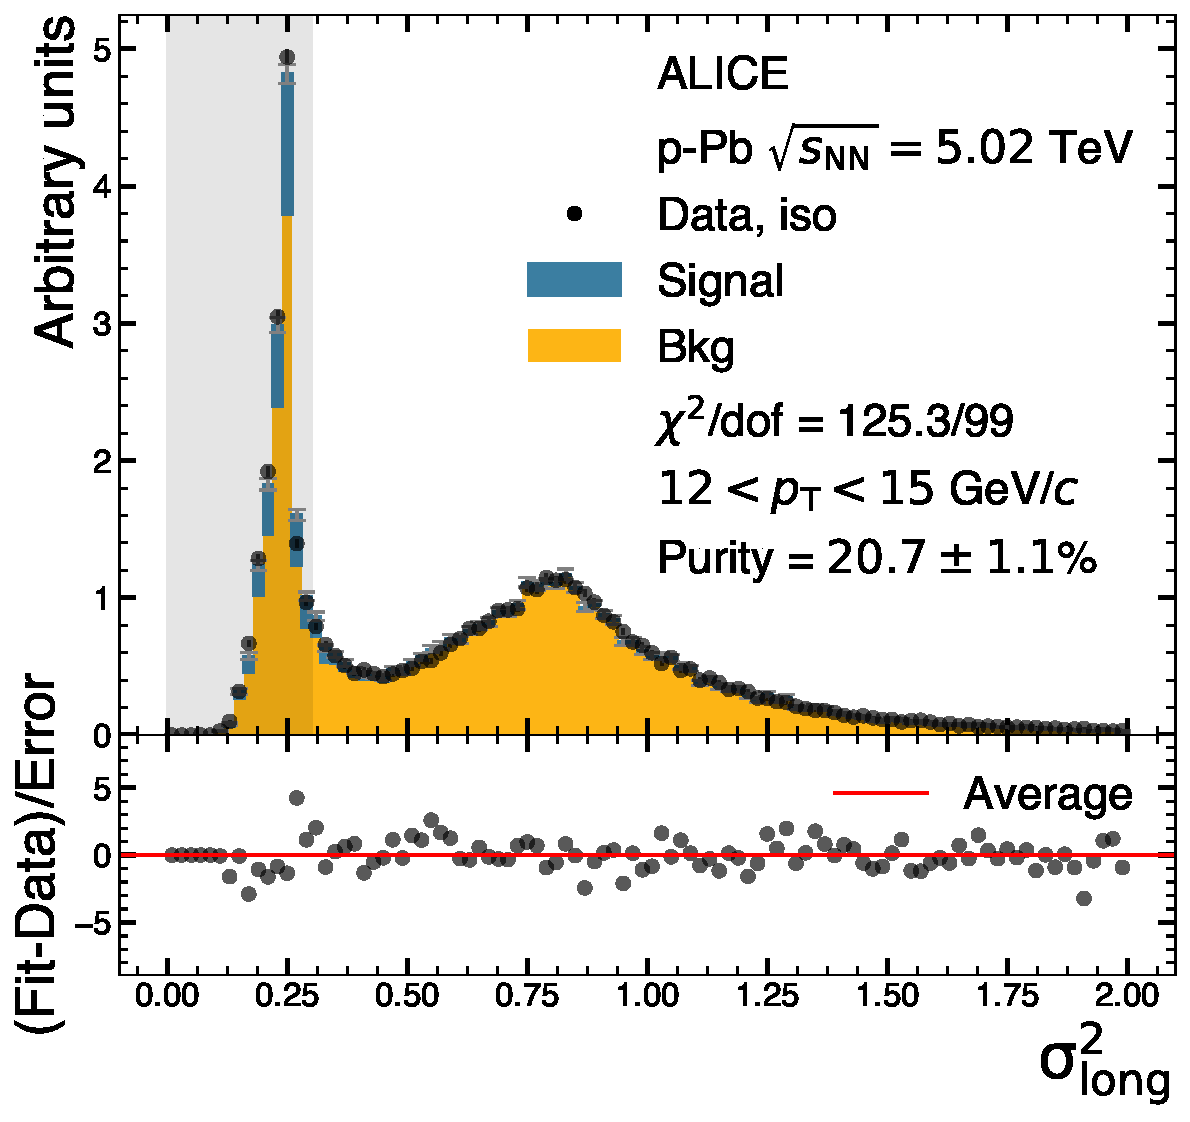
\includegraphics[width=0.3\textwidth]{Data_Analysis/Purity/tf-example-p-Pb-cluster_Lambda-12-15.pdf}
\\
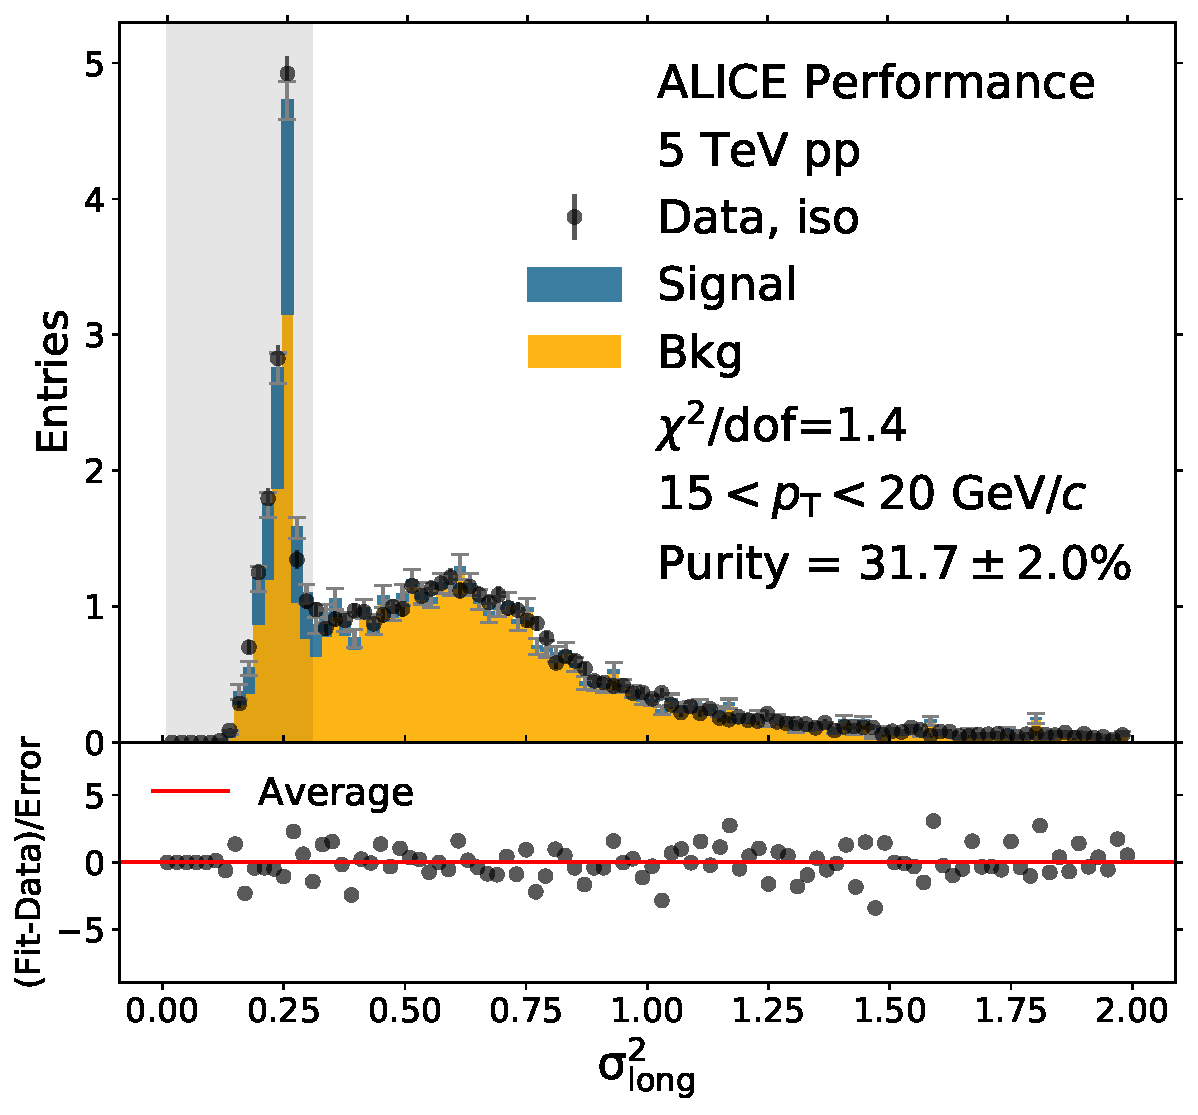
\includegraphics[width=0.3\textwidth]{Data_Analysis/Purity/tf-example-pp-cluster_Lambda-15-20.pdf}
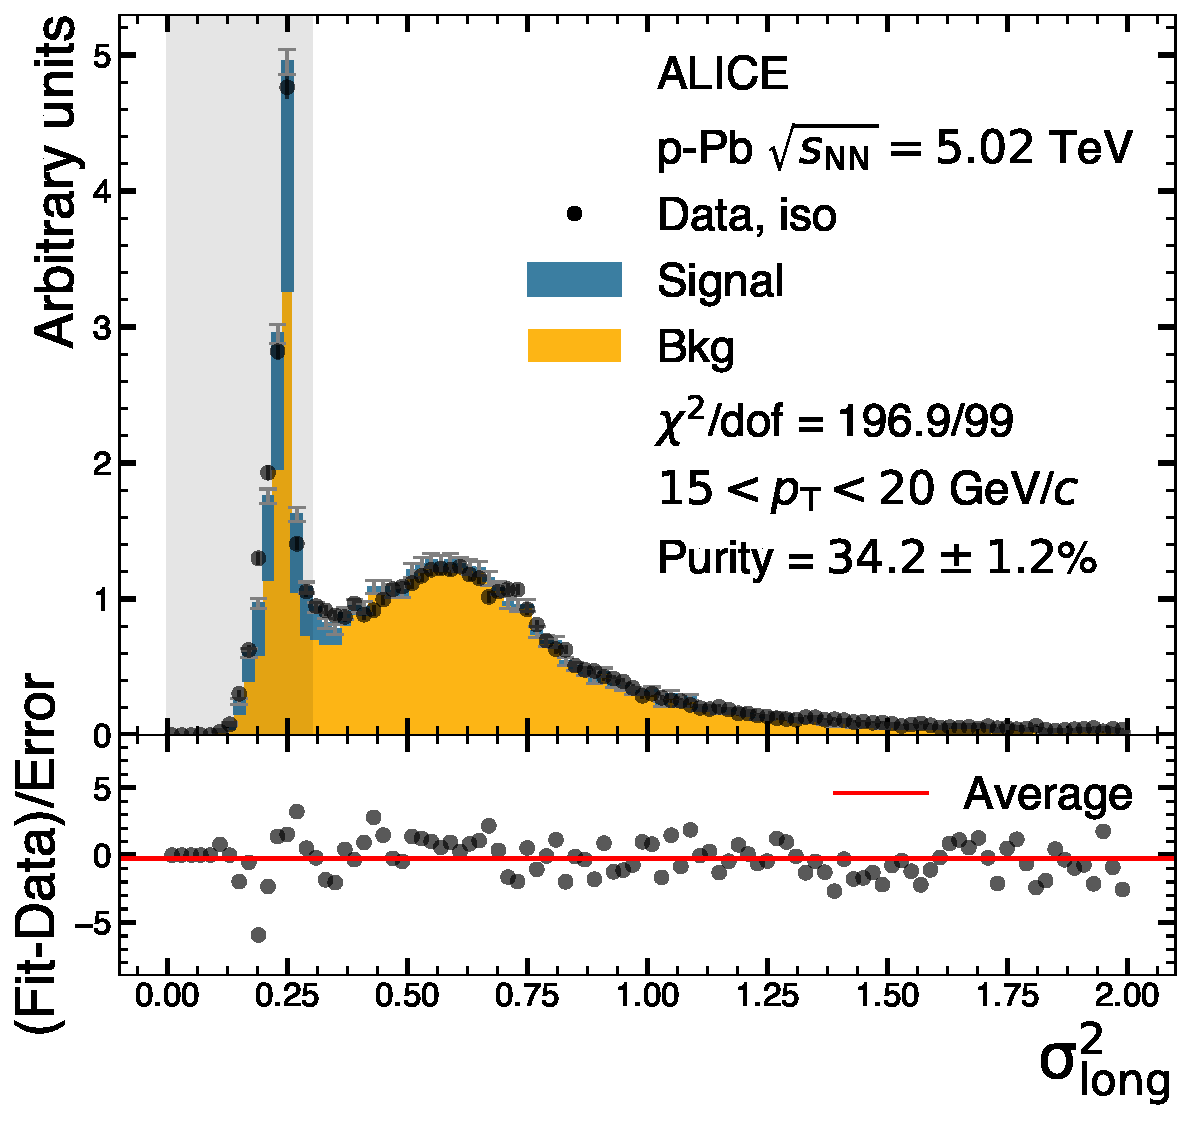
\includegraphics[width=0.3\textwidth]{Data_Analysis/Purity/tf-example-p-Pb-cluster_Lambda-15-20.pdf}
\\
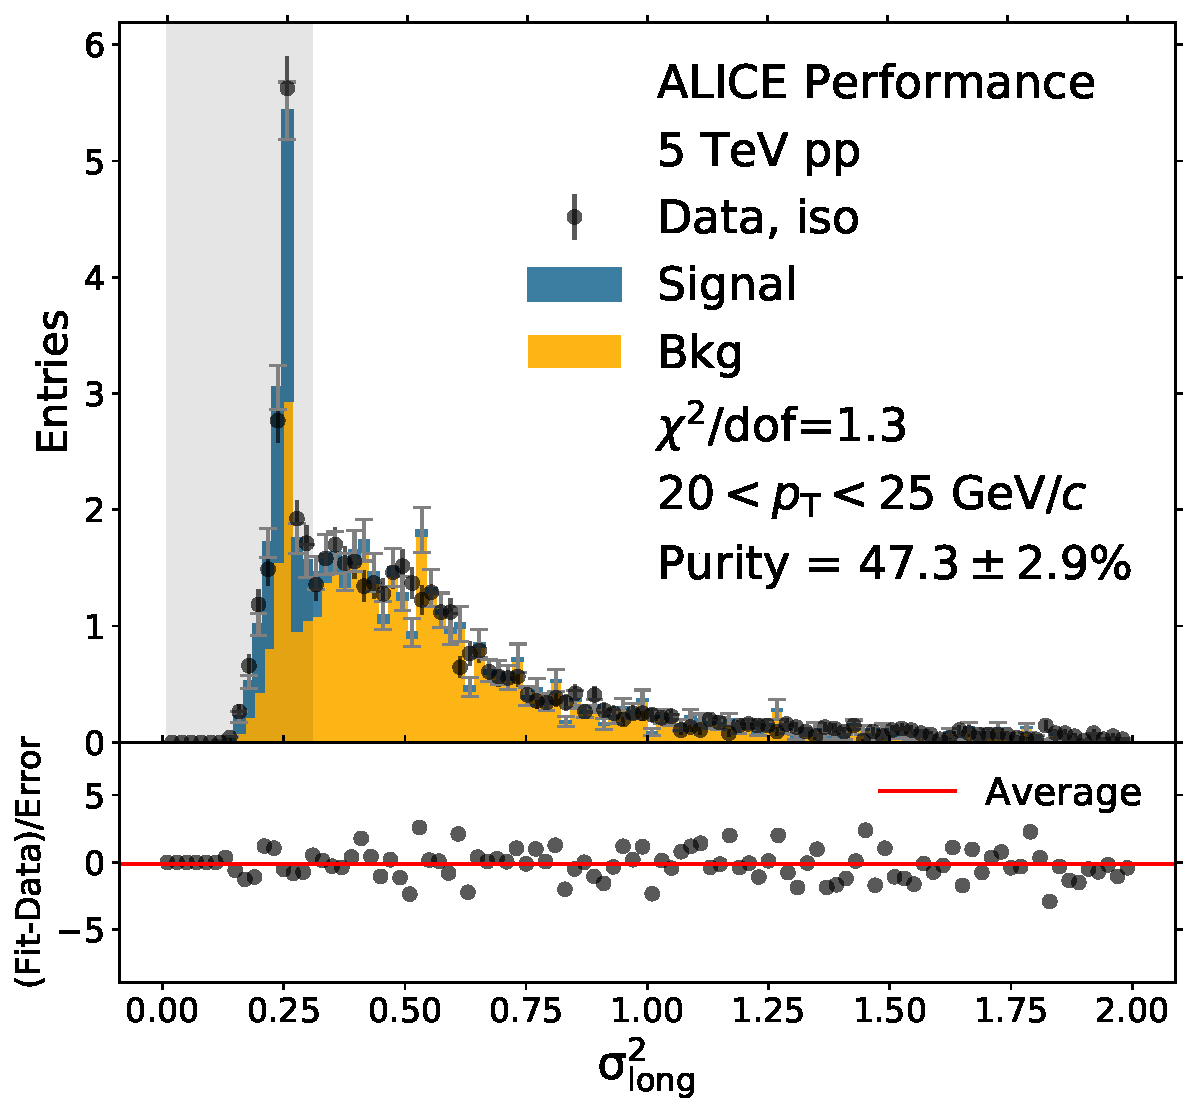
\includegraphics[width=0.3\textwidth]{Data_Analysis/Purity/tf-example-pp-cluster_Lambda-20-25.pdf}
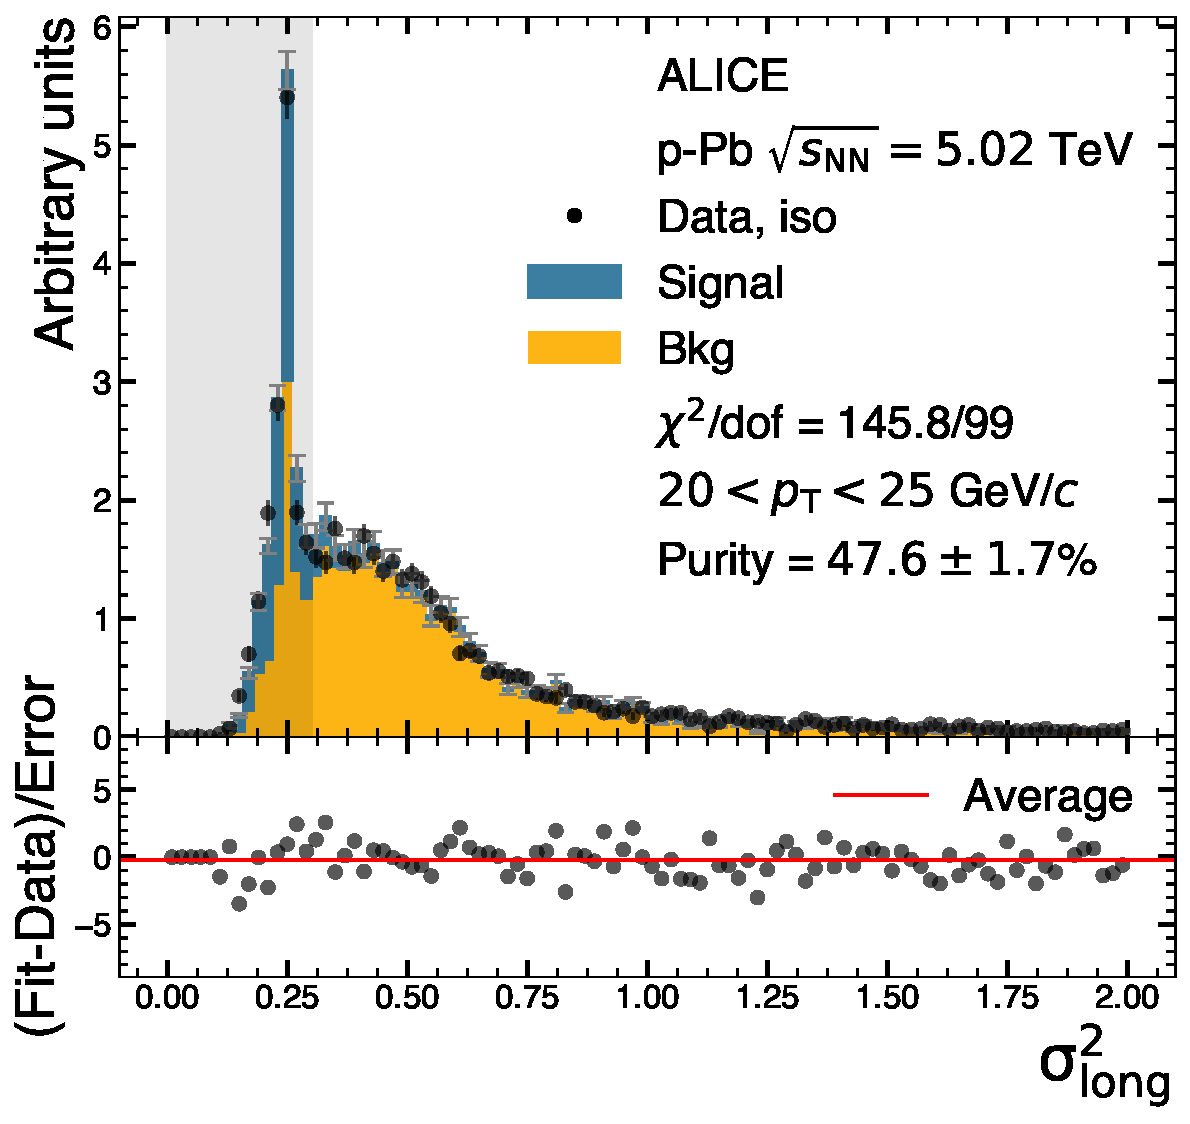
\includegraphics[width=0.3\textwidth]{Data_Analysis/Purity/tf-example-p-Pb-cluster_Lambda-20-25.pdf}
\\
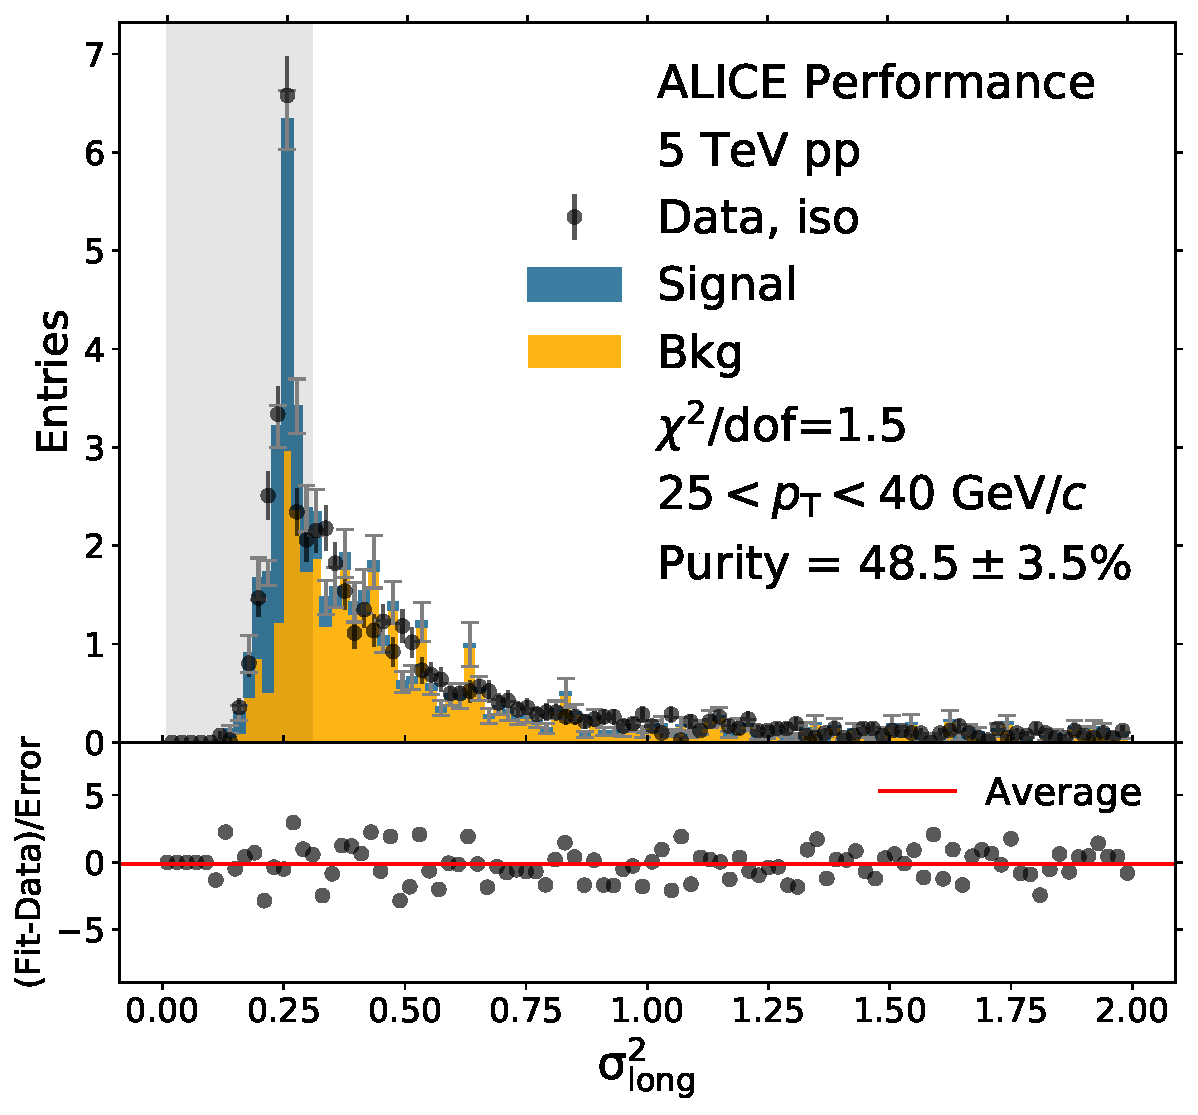
\includegraphics[width=0.3\textwidth]{Data_Analysis/Purity/tf-example-pp-cluster_Lambda-25-40.pdf}
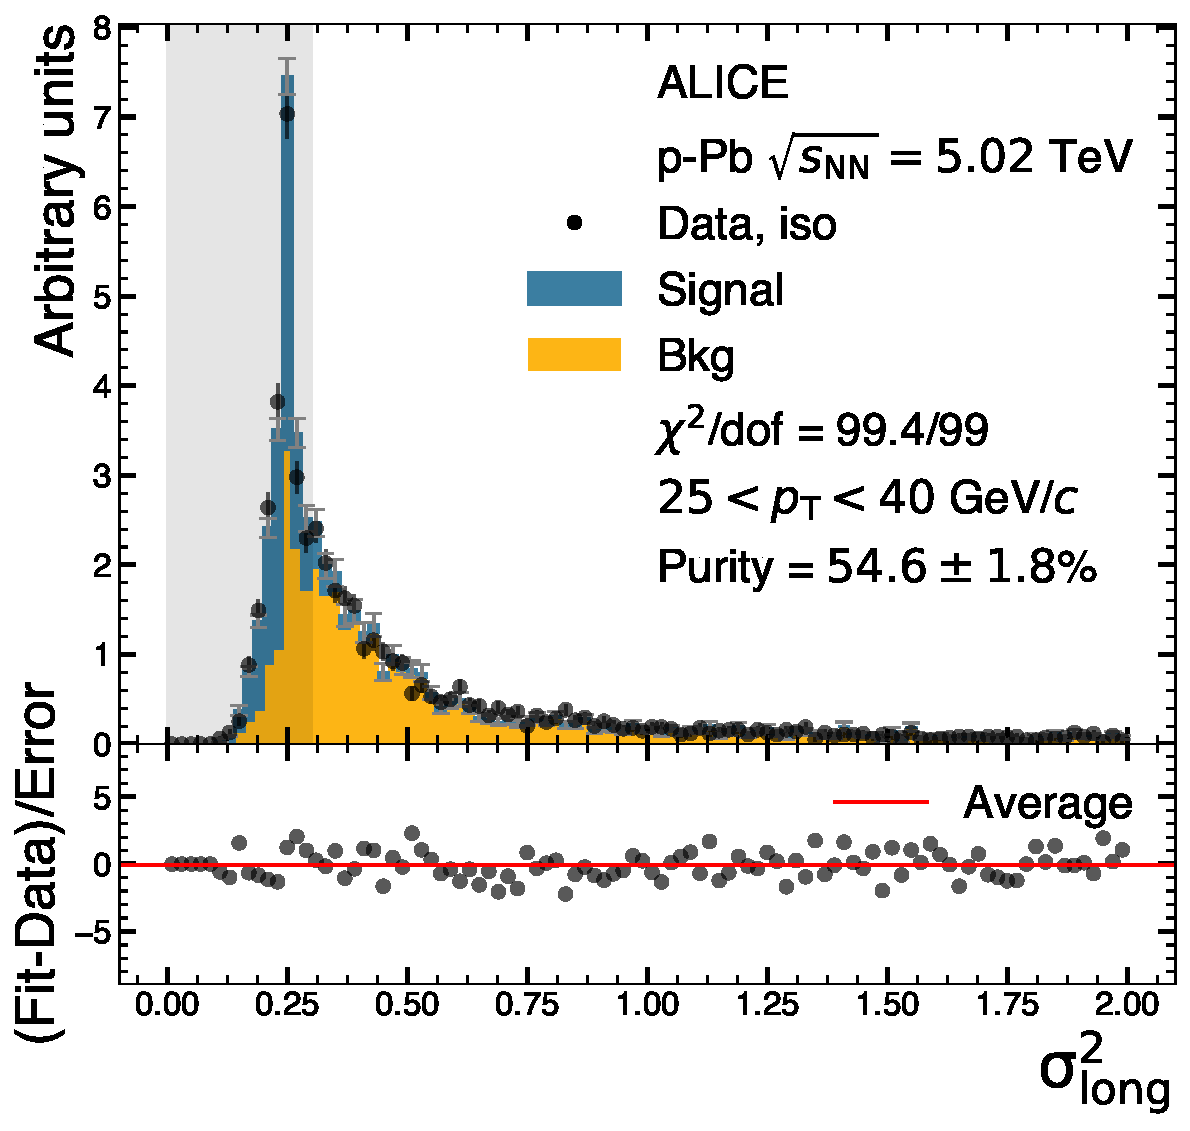
\includegraphics[width=0.3\textwidth]{Data_Analysis/Purity/tf-example-p-Pb-cluster_Lambda-25-40.pdf}
\caption{\lambdasquare distribution of isolated clusters (black) and template fit results for \pPb~data in various \pt~ranges. The stacked histograms (yellow for background, blue for signal) show the predicted counts corresponding to the best fit. The bottom panels show the normalized residuals of the fit, with the statistical uncertainty on the isolated cluster data and the background template added in quadrature. The gray shaded region indicates the signal region for the isolated-photon selection. See text for additional details.}
\label{TemplateFit}
\end{figure}

%\begin{table}
%   \caption{Impact of the \gammaiso selection variations on purity measurement on pp and \pPb~data. The nominal isolation selection is changed to $\iso<$1.50 $\pm$ 0.25 \GeVc; the nominal shower-shape selection is changed to  $\lambdasquare<0.30 \pm 0.03$}
%   \label{tab:variationspurity}
    % \begin{tabular*}{1.0\columnwidth}{@{\extracolsep{\fill}}l|llllll@{}}
    % 	\hline
    % 	 & Nominal & $\iso < 1.25$ \GeVc & $\iso < 1.75$ \GeVc & $\lambdasquare < 0.27$ & $\lambdasquare < 0.33$ \\
    % 	\hline
    % 	pp data & & & & & \\
    % 	\hline
    % 	12--15 \GeVc & 16.9 & 18.2 & 15.9 & 16.5 & 16.9 \\
    % 	15--20 \GeVc & 29.5 & 31.0 & 28.0 & 29.3 & 29.1 \\
    % 	20--25 \GeVc & 46.8 & 48.4 & 45.4 & 49.1 & 44.9 \\
    % 	25--40 \GeVc & 48.0 & 49.3 & 46.7 & 55.9 & 45.1 \\
    % 	\hline
    % 	p-Pb data & & & & & \\
    % 	\hline
    % 	12--15 \GeVc & 20.7 & 21.5 & 19.7 & 20.2 & 20.5 \\
    % 	15--20 \GeVc & 34.2 & 35.5 & 33.1 & 34.3 & 33.6 \\
    % 	20--25 \GeVc & 47.6 & 49.0 & 46.5 & 51.7 & 44.9 \\
    % 	25--40 \GeVc & 54.6 & 56.8 & 52.8 & 62.1 & 51.1 \\
    % 	\hline
    % \end{tabular*}
%\end{table}


\begin{figure}[h]
\center
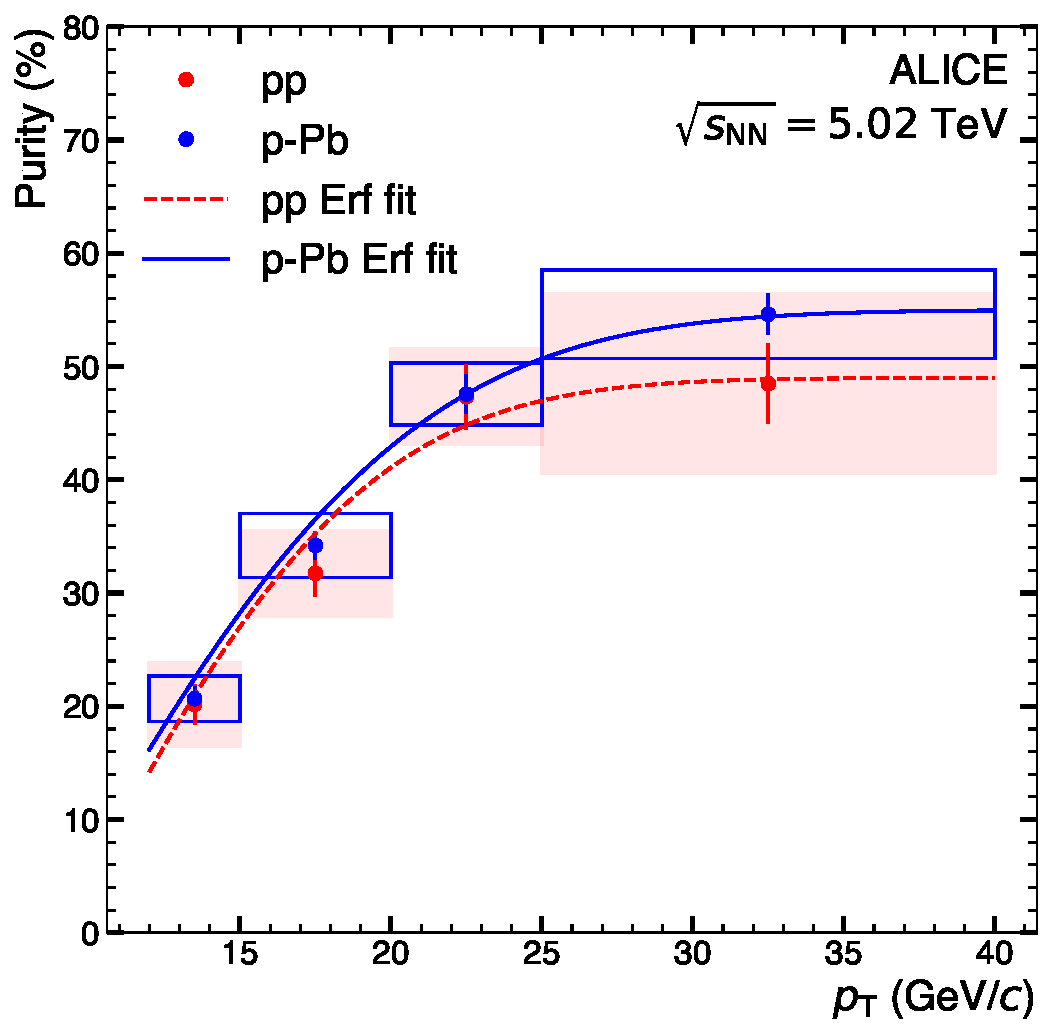
\includegraphics[width=0.8\textwidth]{Data_Analysis/Purity/purity.pdf}
\caption{Purity of the $\gammaiso$ sample as a function of transverse momentum for pp (red) and \pPb~(blue) data. The error bars represent statistical uncertainties only. The red shaded area represents systematic uncertainties in pp, while the blue empty boxes represent systematic uncertainties in \pPb. The smooth lines correspond to a three-parameter error function fit to the data.}
\label{fig:purityresults}
\end{figure}

The purities in the pp and \pPb~datasets are compatible within the uncertainties. The $\text{Weights}(\lambdasquare)$ function for different \pt~ranges is shown in Appendix~\ref{sec:MCbasedcorrection} and the evaluation of the systematic uncertainty associated with this correction is described in Section~\ref{sec:puritysystematics}. 
\FloatBarrier
%%%%%%%%%%%%%%%%%%%%%%%%%%%%%%%
% \subsection{Systematic uncertainties of the purity measurement}


% \section{Particle Selection}

% \subsection{Photon Selection}
% \label{sec:photon_selection}
% \subsection{Charged Hadron Selection}
\section{Charged Particle Tracking}
\label{sec:tracking}
The detectors usually responsible for measuring the charged hadrons in this analysis are the ALICE Inner Tracking System (ITS) and Time Projeciton Chamber (TPC). During the 13def and 17q periods, however, the TPC was either not read out or compromised due to space-charge distortions, mentioned in Sec.~\ref{sec:tpc}. As a result, this analysis relies on only the ITS for track reconstruction.

ITS-only tracking in ALICE is new for this flavor of analysis. As a result, the charged-particle $\pt$-spectrum using ITS-only tracking is compared to the normal TPC+ITS tracking in the data-taking period when the TPC was active and free of space-charge distortions (the low-luminosity 13b data-taking period at 5 TeV \pPb~minimum-bias data) as well as with published ALICE measurements~\cite{Acharya:2018qsh} that use the same dataset (a more thorough comparison to published ALICE data is done in Sec.~\ref{sec:tracking_published_comparision}).

The combined effect of tracking efficiency, fake rate, and track momentum smearing corrections are calculated using MC simulations, and validated by the comparison to the established hybrid-tracking method in ALICE. The comparison to hybrid tracking also serves as an estimate of the systematic uncertainties due to mis-modeling of the tracking performance.

To study the performance of ITS-only tracking, minimum bias \pPb~events for both data and Monte Carlo. The Monte Carlo simulations used for this section are LHC13b2\_efix\_p1, a \textsc{DPMJET} simulation anchored to LHC13b,c and LHC17l3b, a pp \textsc{Pythia8} simulation anchored to LHC17p. The events are sampled from the LHC13b period and the datasets from \cite{Acharya:2018qsh}, as mentioned previously. Only events with the minimum bias trigger (CINT7) that also the vertex and pileup selections described in Section~\ref{sec:eventselection}. The tracks reconstructed from the ITS (''ITS-only tracks''), are compared with tracks reconstructed from information obtained from both the TPC and ITS (''TPC+ITS tracks'', or ''hybrid'' tracking). Here, ITS-only tracks are reconstructed in a \textit{stand-alone} way and are not simply the ITS-segment of a ITS+TPC track.

In order to select good-quality tracks emerging from the primary vertex while maintaining a high efficiency, each track is required to satisfy the cuts summarized in Table ~\ref{tab:track_cuts}. A set of standard PWG-JE cuts are applied to all tracks, and additional track cuts are applied depending on whether the track is a TPC+ITS track or an ITS-only track. 

\begin{table}[h]
   \centering
      \caption{Summary of the cuts used in Track Selection.}	
   \label{tab:track_cuts}
   \begin{tabular*}{1.0\columnwidth}{@{\extracolsep{\fill}}l|c@{}}
      	\hline
 		\textbf{Common Cuts}\\
        %\textbf{ITS--Only Cuts}\\
        \hline
        track $\eta$ & $|\eta| < 0.8$\\
        track $\pt$ & $\pt \geq 0.150$ \GeVc\\
        SetMaxDCAToVertexXY & 2.4 cm\\
        SetMaxDCAToVertexZ & 3.2 cm\\
        SetDCAToVertex2D & TRUE\\
		\hline \hline
        \textbf{TPC+ITS Cuts}\\
        \hline
        SetMinNClustersTPCPtDep & 70.+30./20.*x, 20.0\\ 
        SetMinNClustersTPC & 70\\
        SetMaxChi2PerClusterTPC & 4\\
        SetMaxChi2PerClusterITS & 36\\
        SetMaxFractionSharedTPCClusters & 0.4\\
        SetMaxChi2TPCConstrainedGlobal &36 \\
        SetRequireTPCStandAlone & TRUE\\
        SetRequireTPCRefit & TRUE \\
        SetRequireITSRefit & TRUE\\
        SetRequireSigmaToVertex & FALSE \\
        SetAcceptKinkDaughters & FALSE\\
        \hline \hline
        \textbf{ITS--Only Cuts}\\
        \hline
        SetRequireITSPureStandAlone &TRUE\\
        SetMinNClustersITS & 4\\
        SetMaxChi2PerClusterITS & 36\\
        \hline
   \end{tabular*}
\end{table}
\FloatBarrier

\subsection{Efficiency and Fake Rate}
\label{sec:Efficiency_fake_rates}
%The tracking efficiency is calculated from the minimum bias \pPb~simulation (see Table~\ref{tab:MCsamples}).
The tracking efficiency is calculated as the ratio of the number of reconstructed primary particles\footnote{No special tuning of the particle type composition is performed. This typically only matters at low $\pt$ and enforces a small (percent level) correction to the out-of-the-box results.}, $N_{\mathrm{prim,rec}}(p_\mathrm{T})$, to the number of generated primary particles, $N_{\mathrm{prim,gen}}$. The truth-to-reconstructed matching is done following the standard ALICE method.
\begin{equation}\label{eq:eff}
\epsilon (\pt^{\mathrm{true}}) = \frac{N_{\mathrm{prim,rec}}(\pt^{\mathrm{true}})}{N_{\mathrm{prim,gen}}(\pt^{\mathrm{true}})}.
\end{equation}

Shown in Eq.~\ref{eq:eff}, the simulated or ''truth'' transverse momentum, $\pt^{\mathrm{true}}$, is used in both the numerator and denominator in order cancel effects of efficiency from bin-migration due to momentum smearing.

The numerator of Equation~\ref{eq:eff} is restricted for charged particles with generated pseudorapidity in the range $|\eta^{\mathrm{true}}|<0.8$ and azimuth $0<\varphi^{\mathrm{true}}<2\pi$. Therefore, the correction factor accounts for both geometrical acceptance, detector inefficiencies, and dead channels.  

Fake tracks are defined as reconstructed tracks that do not match to a truth particle. The fake rate is calculated by taking the ratio of the number of fake tracks to the total number reconstructed tracks. It is parametrized as a function of the reconstructed transverse momentum of the track, $\pt^{\mathrm{reco}}$:

\begin{equation}\label{eq:fakes}
\mathrm{fake rate} (\pt^{\mathrm{reco}}) = \frac{N_{\mathrm{unmatched}}(\pt^{\mathrm{reco}})}{N_{\mathrm{all reco}}(\pt^{\mathrm{reco}})}.
\end{equation}

Figure~\ref{fig:tpcEff} shows the efficiency and the fake rates for the TPC+ITS and ITS only tracks. In both cases the efficiency grows with $\pt$ up to about 1 \GeVc~where it dips and it reaches a plateau value with no significant $\pt$ dependence. The efficiency starts at about 57$\%$ for the TPC+ITS tracks and at 70$\%$ for ITS-only tracks at 150 MeV and plateaus at 84\% and 88\% respectively. %The plateau is calculated by applying a constant fit from {2 $< \pt <$$ 20 GeV/c$}. 

The lower efficiency for the TPC+ITS tracks compared to ITS-only tracks is expected since the former requires a matching between ITS and TPC track segments, which has some inefficiency. This study shows that the matching efficiency is high at large $\pt$ but leads to substantial differences at low $\pt$.  

%The decrease in the tracking efficiency by about 2--5$\%$ in the range 1--3 \GeVc~is due to the fact that above about 1 \GeVc, tracks are almost straight and can be contained completely in the dead areas between TPC sectors or in ITS dead staves. Therefore, at high $\pt$ the efficiency is dominated by geometry and thus has a constant value.

The fake rate for the TPC+ITS tracks is less than a percent over the entire range shown. In comparison, the fake rate is larger in the ITS-only tracks. It is below 5\% up to 5 \GeVc, and it grows roughly linearly and reaches 15\%  at 10 \GeVc. The higher fake rate is due to the much lower number of clusters associated with ITS-only tracks (maximum of 6) than to TPC+ITS tracks (minimum of 70).
\begin{figure}[h]
\center
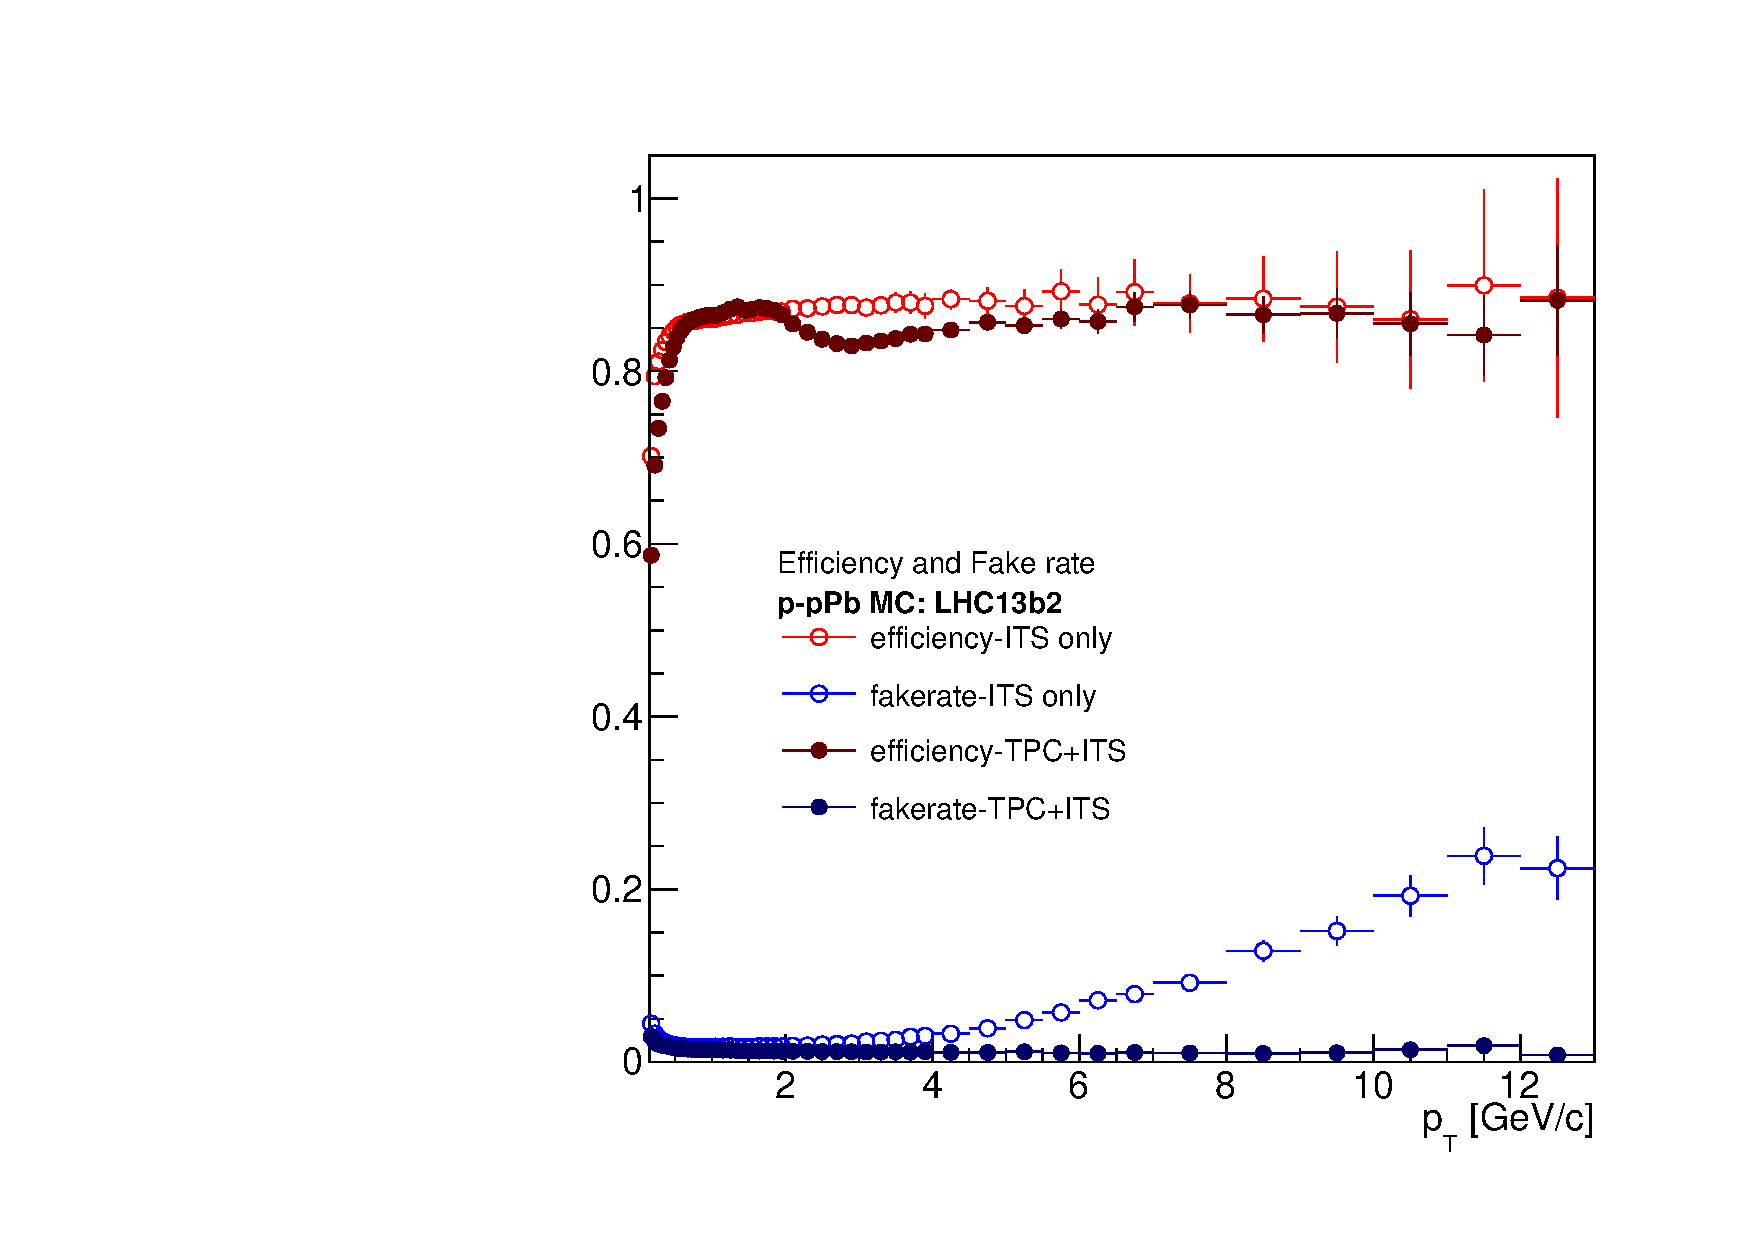
\includegraphics[width=0.7\textwidth]{Data_Analysis/Tracking/HybridAndITS_Eff_fakerate_pPb_lowpt.pdf}
\caption{Efficiency and fake rate for combined TPC+ITS tracking (filled circles) and ITS-only tracking (open circles) obtained with \pPb~simulation. The error bars represent statistical uncertainty only.}
\label{fig:tpcEff}
\end{figure}

%The efficiency and fake rate between pp and \pPb~are rather similar. Figure~\ref{fig:ppPb_eff} shows the comparison between the pp efficiency and \pPb~efficiency as well as the fake rate for pp and the fake rate for \pPb~for ITS-only tracks. The pp efficiency was calculated using the 17l3b Monte Carlo simulation. %The pp efficiency plateaus at 85\%, while the \pPb~efficiency is 88\% as mentioned previously. 
%\begin{figure}[h]
%\center
%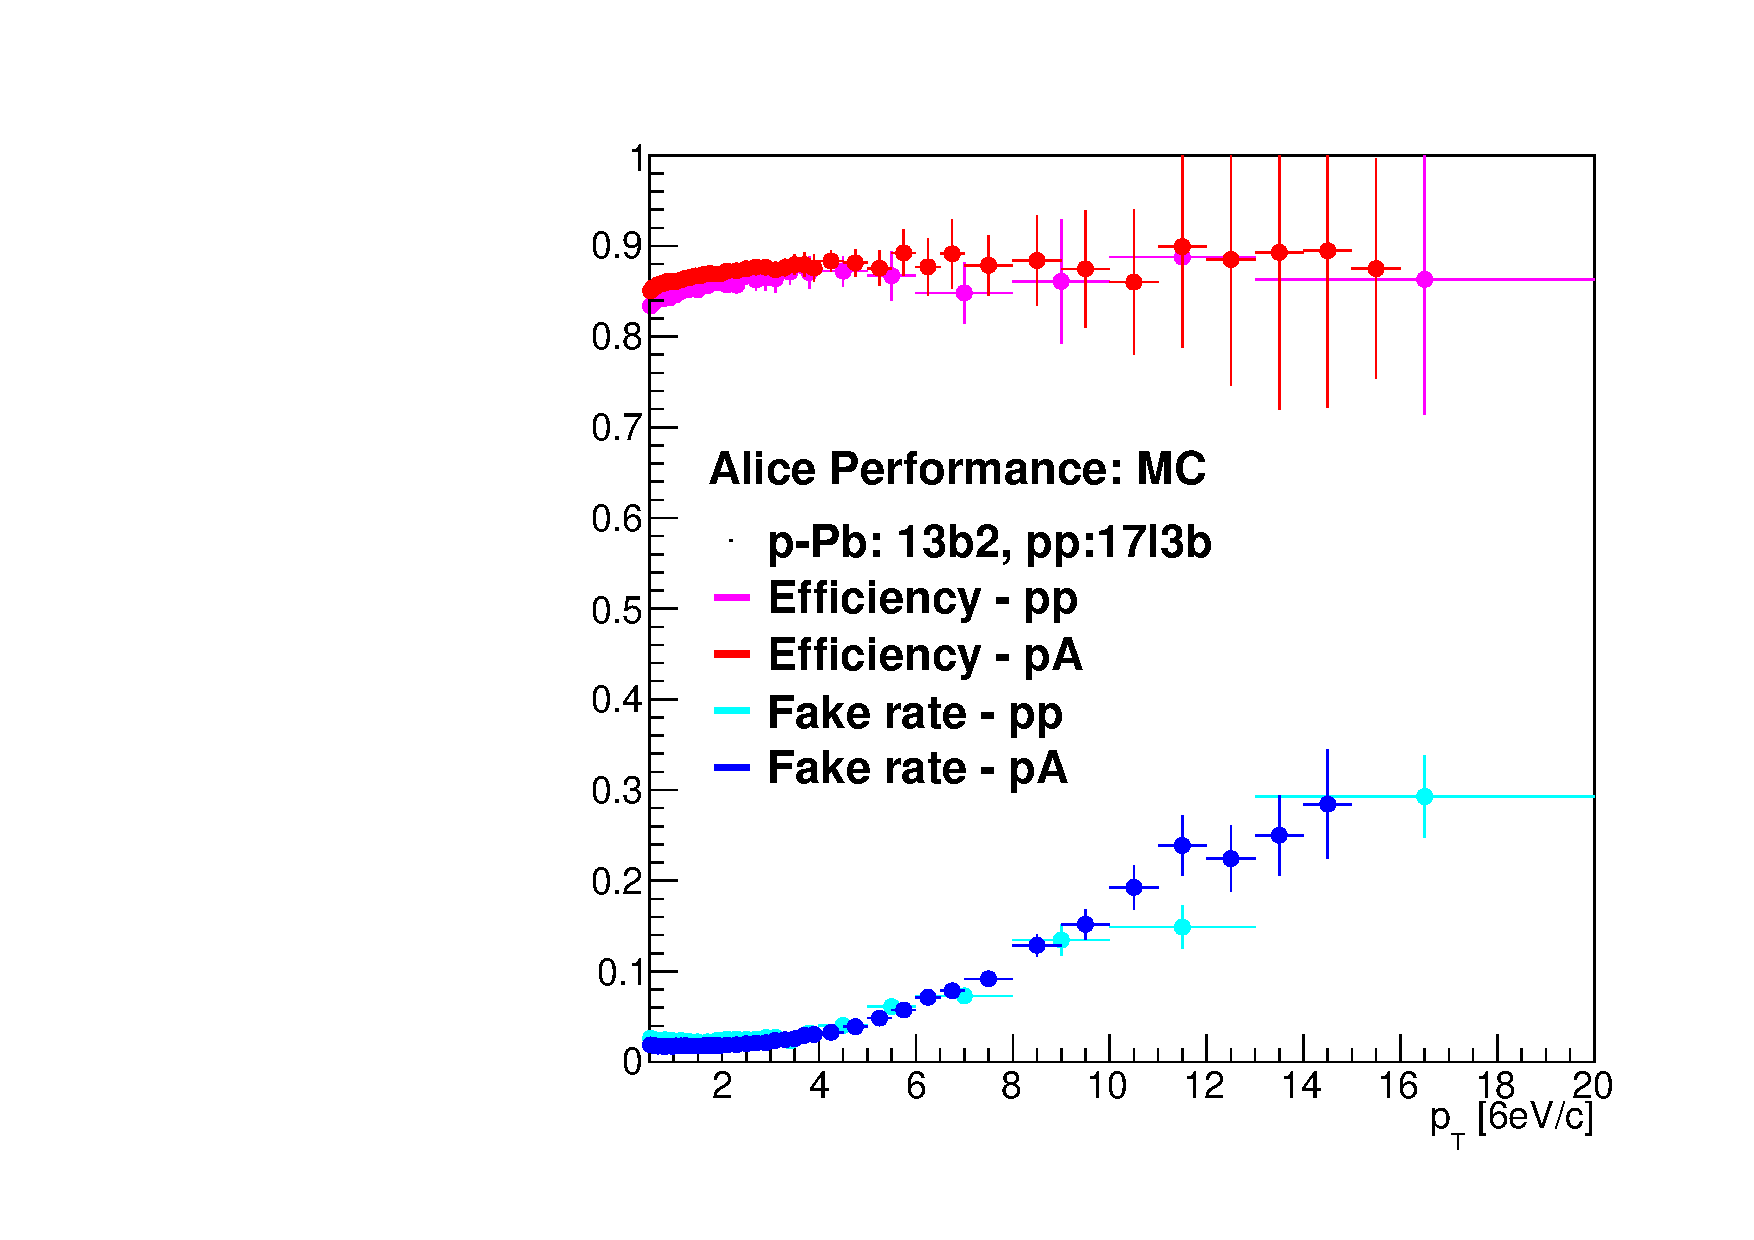
\includegraphics[width=0.7\textwidth]{Tracking/EfficiencyFakeRate_tracking_pApp_compare_halfGeV20GeV_publishedBinning.pdf}
%\caption{Efficiency and fake rate comparison between pp and \pPb~ITS-only tracks. The error bars represent statistical uncertainty only. }
%\label{fig:ppPb_eff}
%\end{figure}
\FloatBarrier

\subsection{Resolution, Response Matrix and Bin Migration}
The main difference between TPC+ITS and ITS-only tracking lies in the much worse momentum resolution of the latter. This is driven by geometry 
and $\int Bdl$ as the TPC covers up to {$z=$258 cm} but the ITS only to {$z=$48 cm}. 

Figure~\ref{fig:resolution} shows the momentum resolution as a function of $\pt^{\mathrm{true}}$ for 
TPC+ITS and ITS-only tracks. The momentum resolution of both increases with \pt; however, the resolution for TPC+ITS never exceeds a relative 2\% below 20 \GeVc, while the ITS-only tracking resolution is about a factor of 7 worse and reaches $\sim$15\% by 10 \GeVc. In both cases the resolution curves have the expected shape: the growth at low momentum is due to multiple-scattering and the linear growth at higher $\pt$ arises from the number and depth of position measurements, and the track bend at the measurement planes. 
\begin{figure}[h]
\center
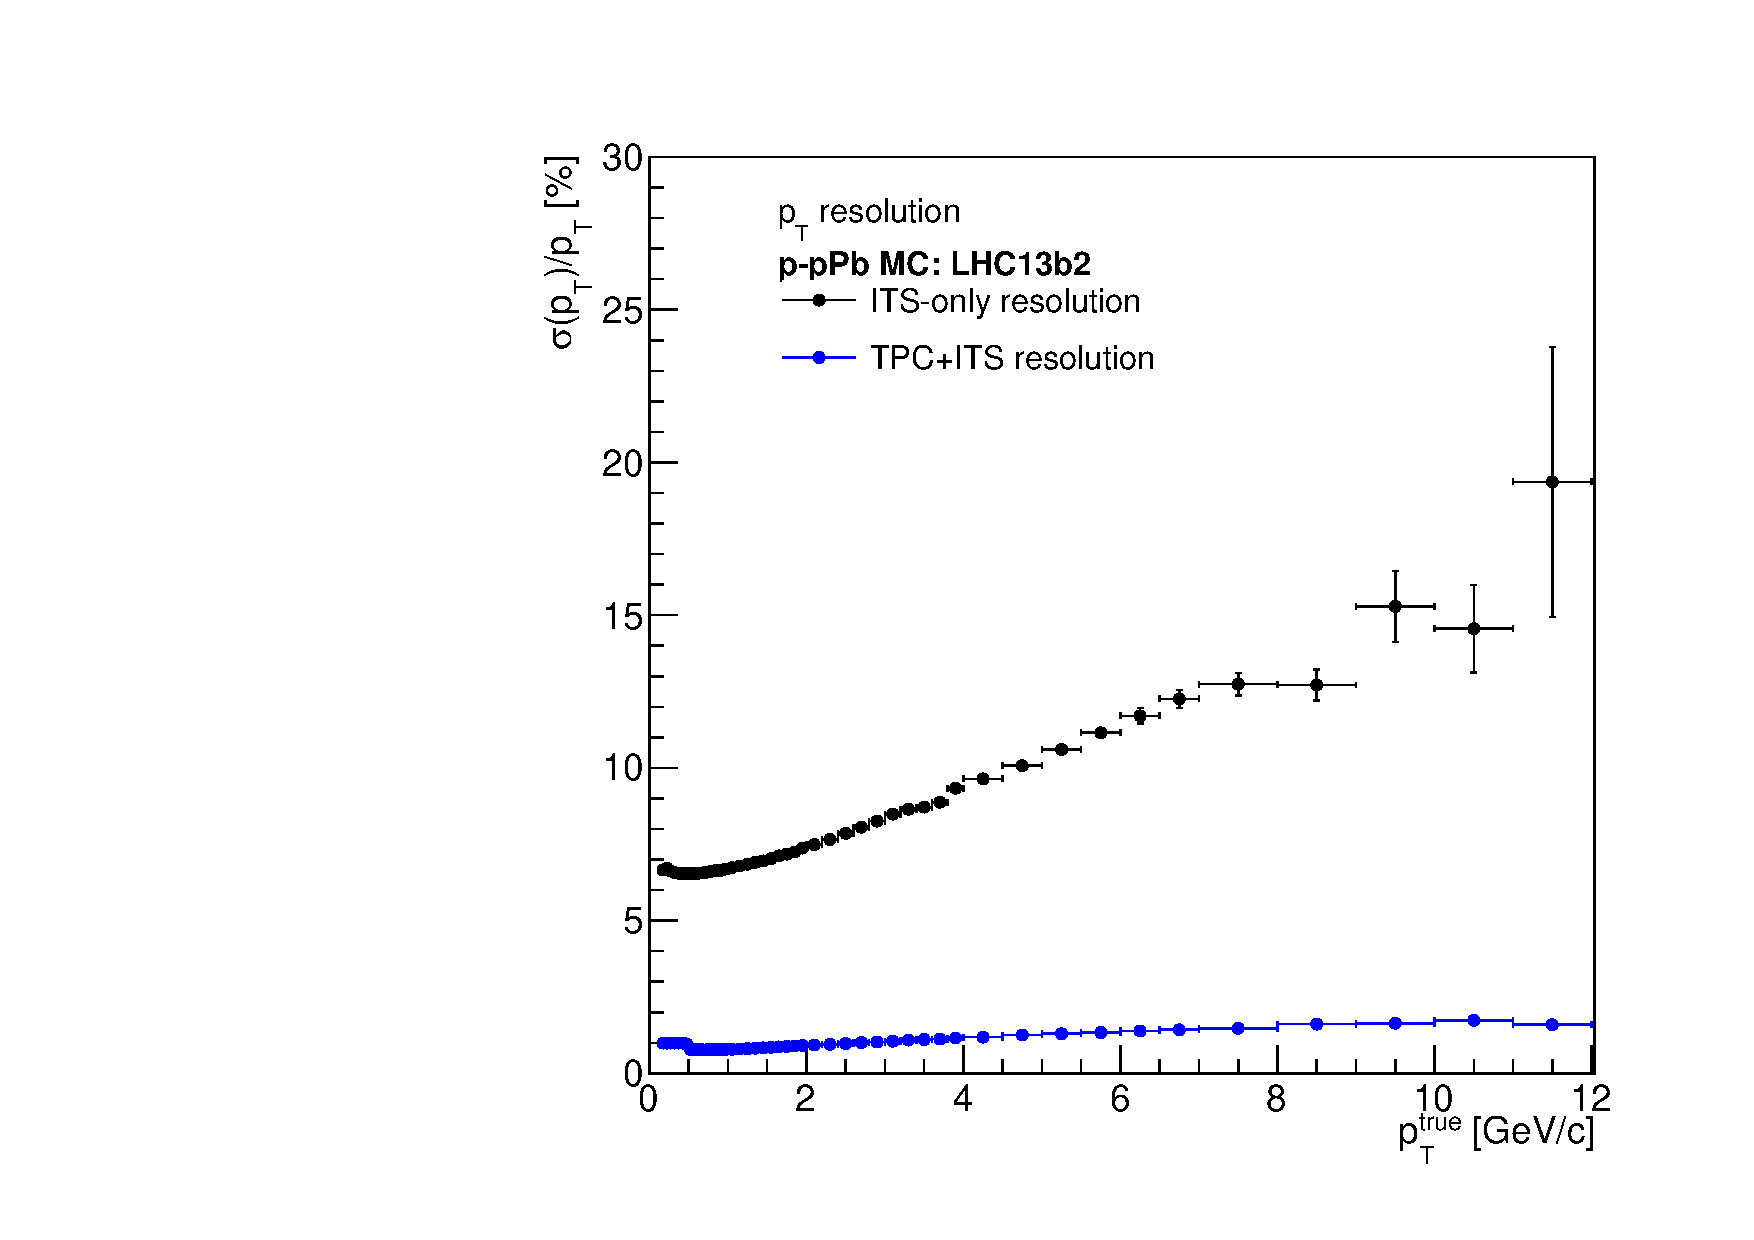
\includegraphics[width=0.7\textwidth]{Data_Analysis/Tracking/HybridAndITS_resolution_lowpt.pdf}\\
\caption{The relative $\pt$ resolution for TPC+ITS tracking and ITS only tracking. The error bar represents statistical uncertainty only.}
\label{fig:resolution}
\end{figure}

The tracking response matrix is defined as the correlation between the reconstructed and generated transverse momentum. This matrix is filled only for reconstructed tracks with a true match; fake tracks are explicitly excluded. Figure~\ref{fig:responseMatrixTPC} shows the response matrix, its one-dimensional projections, and the ratio of true to reconstructed spectra. The ratio of the true to reconstructed spectra is used to correct for bin migration effects, where a track is placed in the wrong \pt bin due to the finite momentum resolution of the detector:

\begin{equation}\label{eq:bin_migration}
\mathrm{bin\:migration} (\pt^{\mathrm{reco}}) = \frac{N_{\mathrm{prim,reco}}(\pt^{\mathrm{true}})}{N_{\mathrm{prim,reco}}(\pt^{\mathrm{reco}})}.
\end{equation}

\begin{figure}[h!]
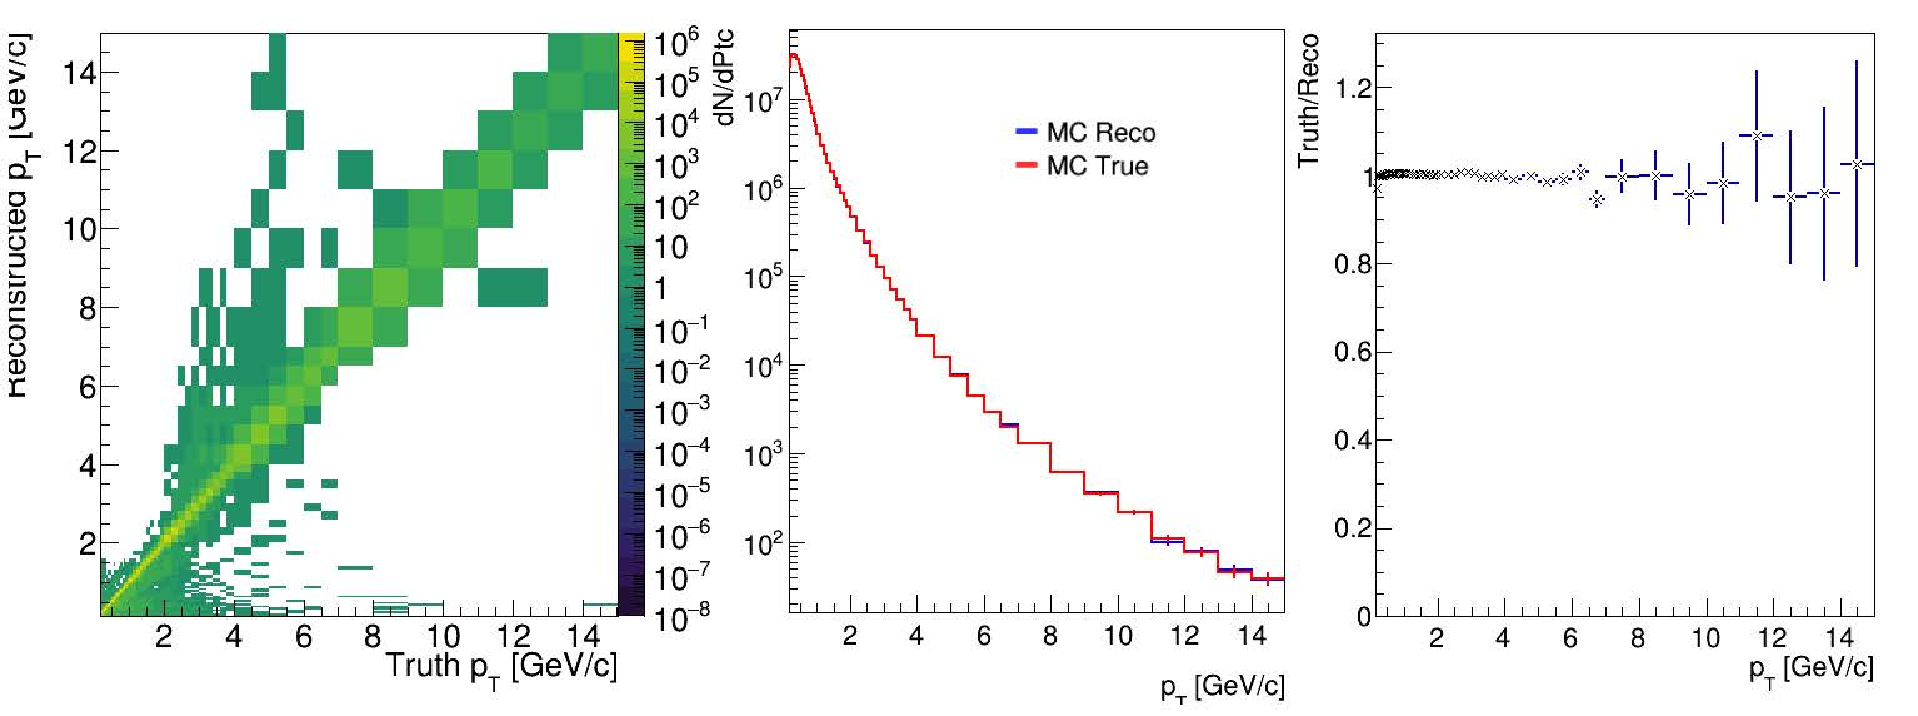
\includegraphics[width=0.98\textwidth]{Data_Analysis/Tracking/Matrix_tracking_tpc_MBMC_0GeV15GeV_dNdPt.pdf}\\
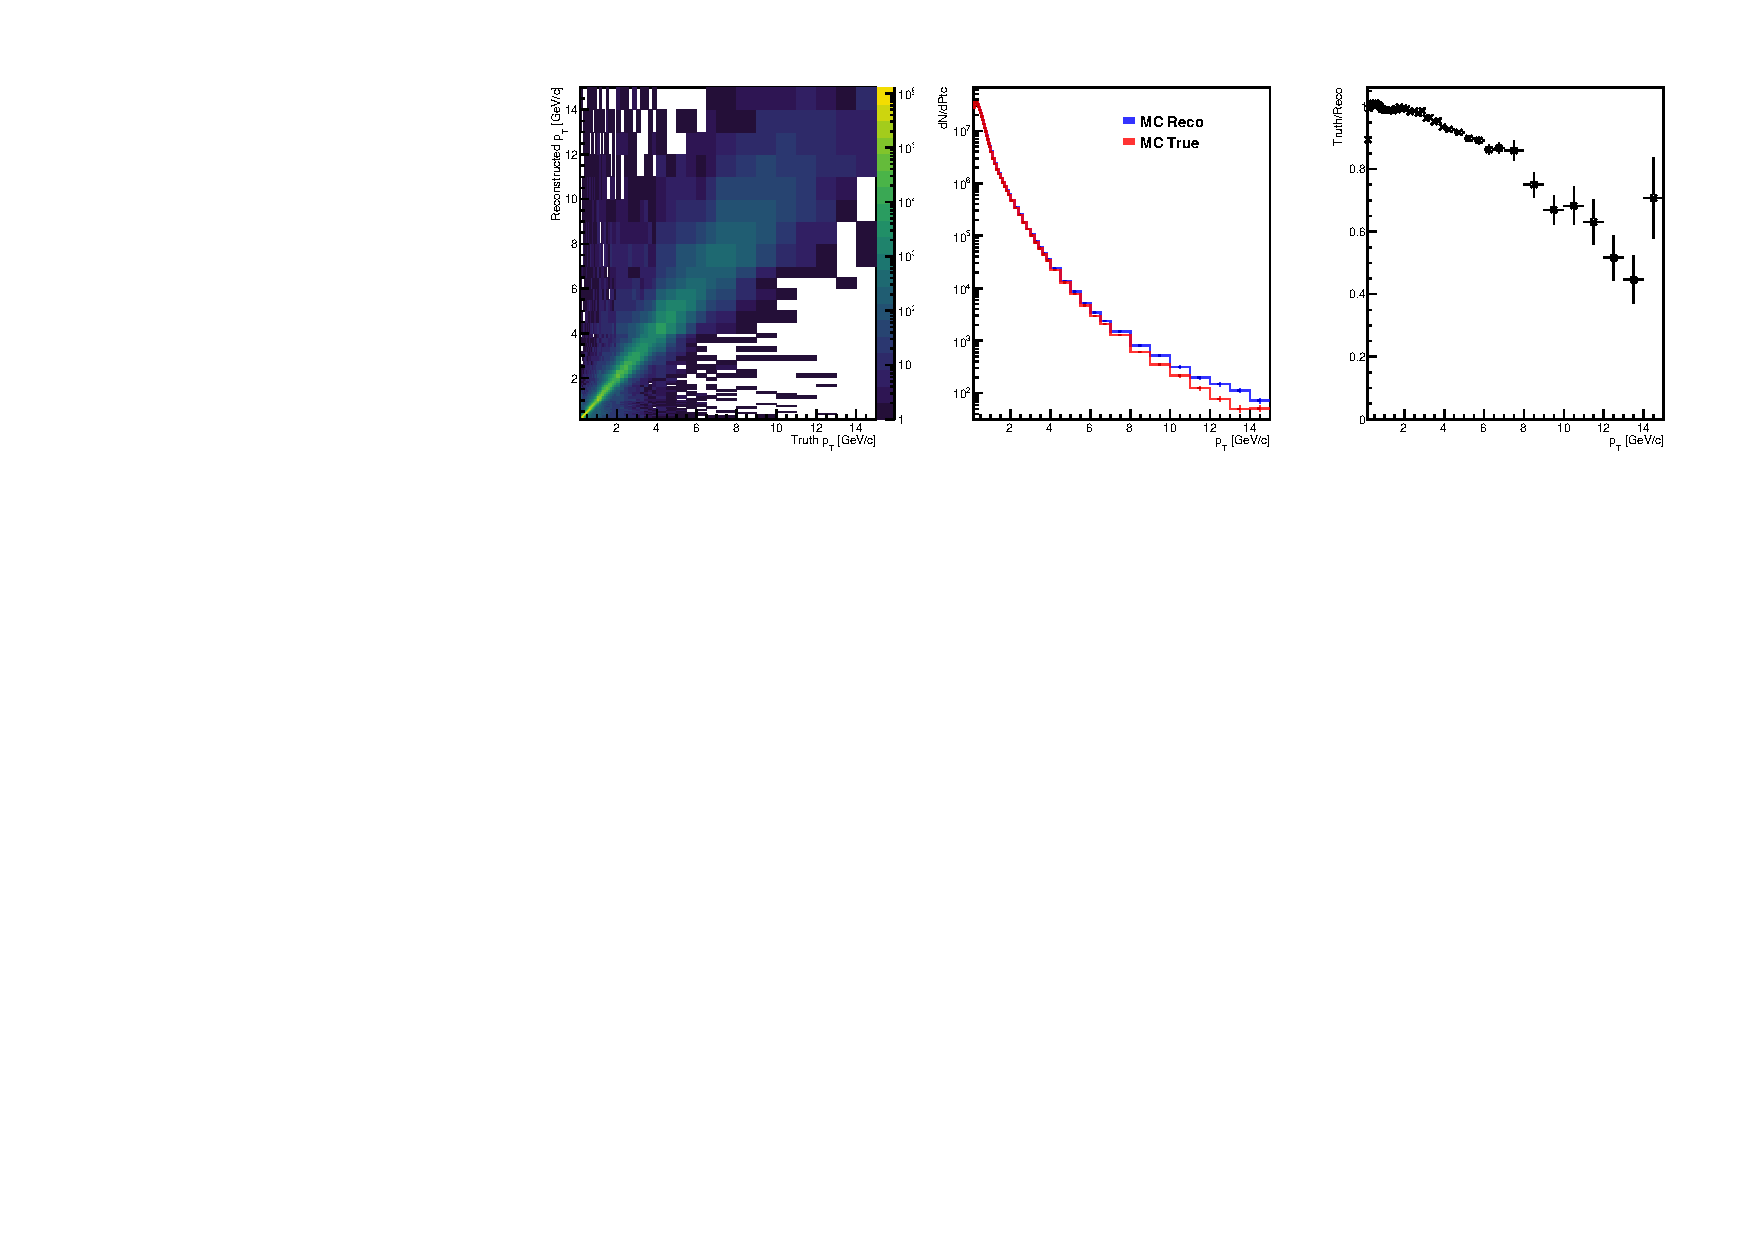
\includegraphics[width=1.0\textwidth]{Data_Analysis/Tracking/Matrix_tracking_its_MBMC_0GeV15GeV_dNdPt.pdf}

\caption{Left panel: correlation matrix between true $\pt$ and reconstructed $\pt$ of tracks reconstructed with TPC+ITS (upper row) and ITS-only (bottom row). Middle panel: projections of the response matrix into the true and reconstructed $\pt$. Right panel: ratio of true to reconstructed spectra. This ratio used as part of the bin-by-bin correction factors.}
\label{fig:responseMatrixTPC}
\end{figure}

The effect of momentum smearing on tracks is clearly visible in the projection plots, where the reconstructed spectrum is significantly harder at high $\pt$. The ratio of truth to reconstructed $\pt$ is very close to unity in the TPC+ITS case, as expected. On the other hand, the ratio deviates significantly from unity in the ITS-only case; it reaches 0.9 at 6 \GeVc~and drops quickly, reaching 0.5 at about 13 \GeVc. The quick drop at high $\pt$ comes mainly from the linear degradation of the relative momentum resolution combined with the fast drop of the true spectrum to produce large effects in the tails. 

The bin migration (b), along with the tracking efficiency ($\epsilon$) and the fake rate (f) are used as the correction factor equation~\ref{eq:track_weight} for the charged hadron tracks; all of them are shown together in Figure~\ref{fig:correctionFactors}. Based on overlapping plot of pp and \pPb, we can see that correction factors are similar for tracks from a pp collision or a \pPb~collision. We conclude that the multiplicity in \pPb~is low enough such that it does not affect tracking performance.  

\begin{equation}\label{eq:track_weight}
w = \frac{1}{\epsilon}(1-f)b
\end{equation}

\begin{figure}[h]
\center
%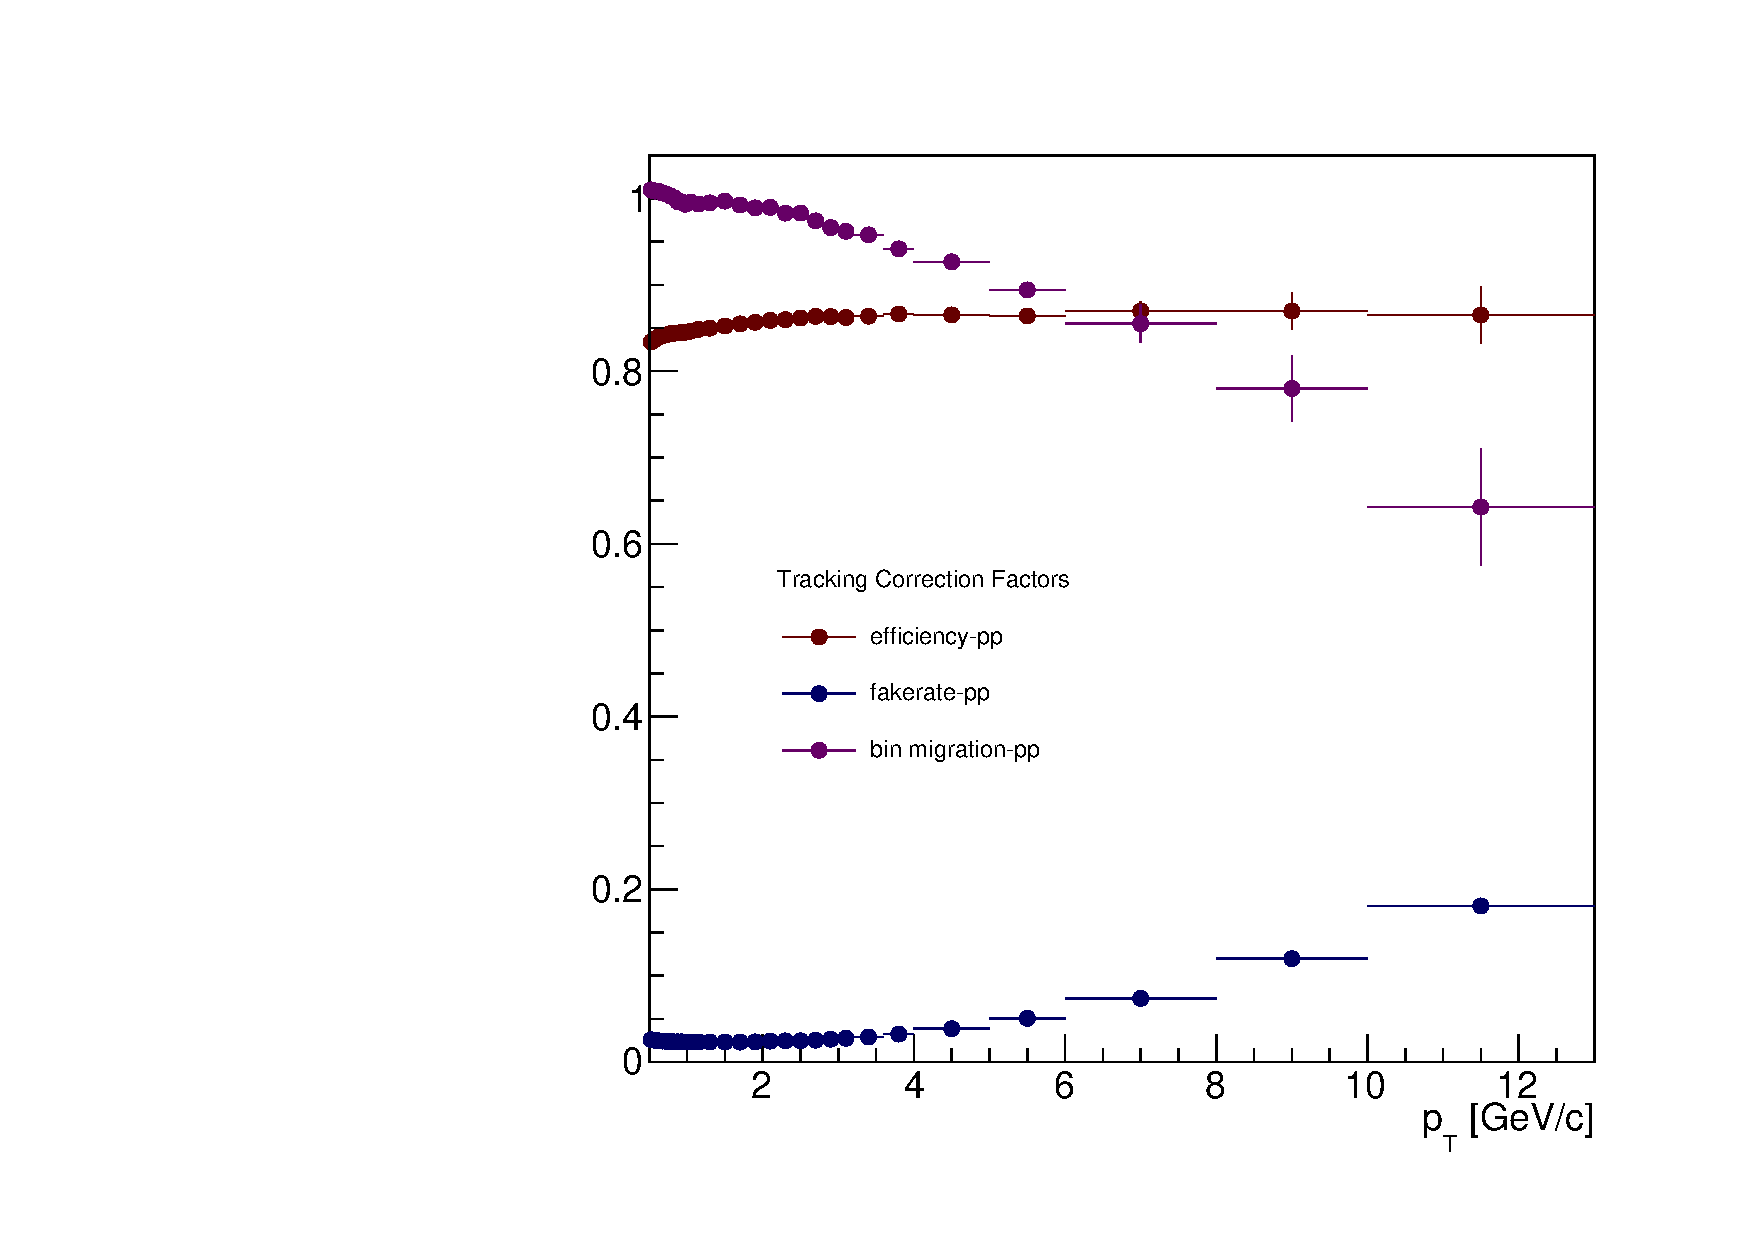
\includegraphics[width=.45\textwidth]{Data_Analysis/Tracking/trackCorrectionFactors_pp.pdf}
%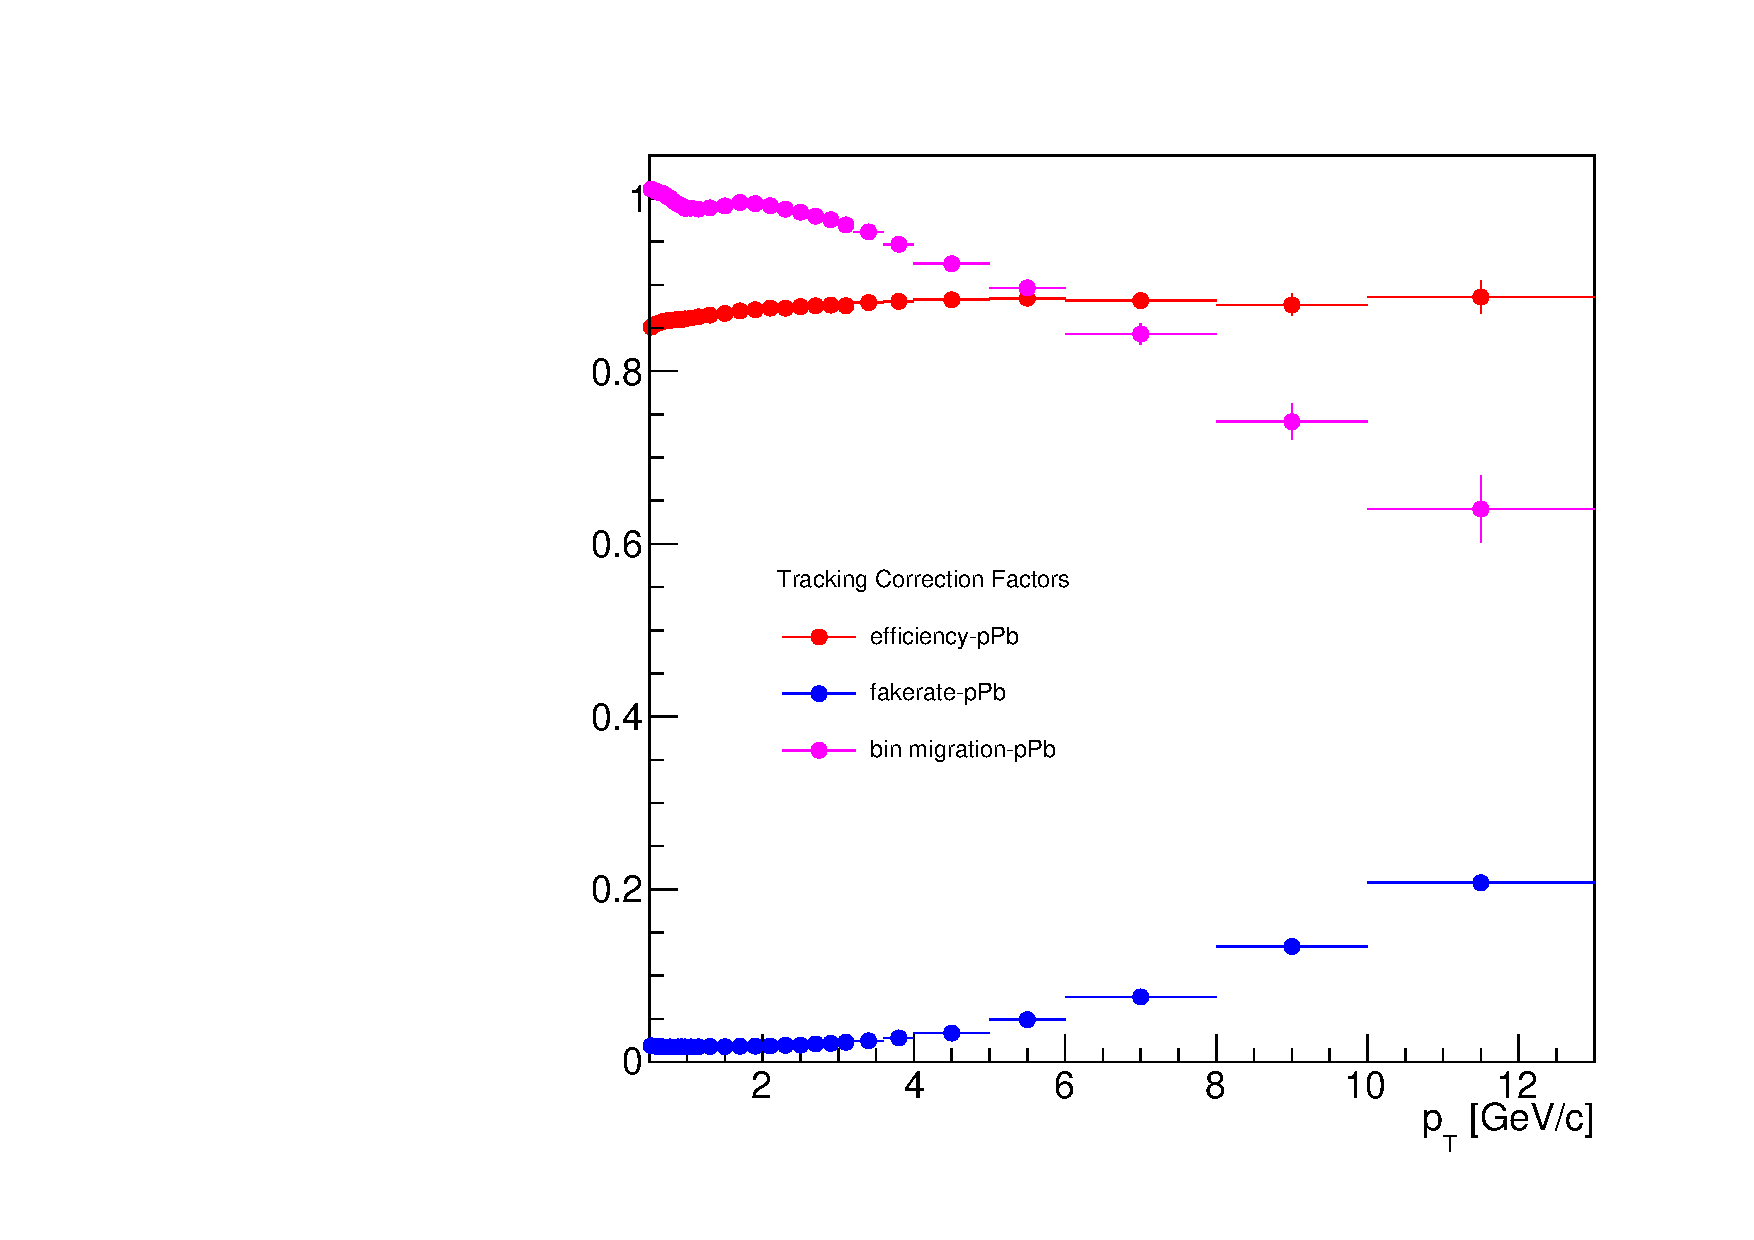
\includegraphics[width=.45\textwidth]{Data_Analysis/Tracking/trackCorrectionFactors_pPb.pdf}
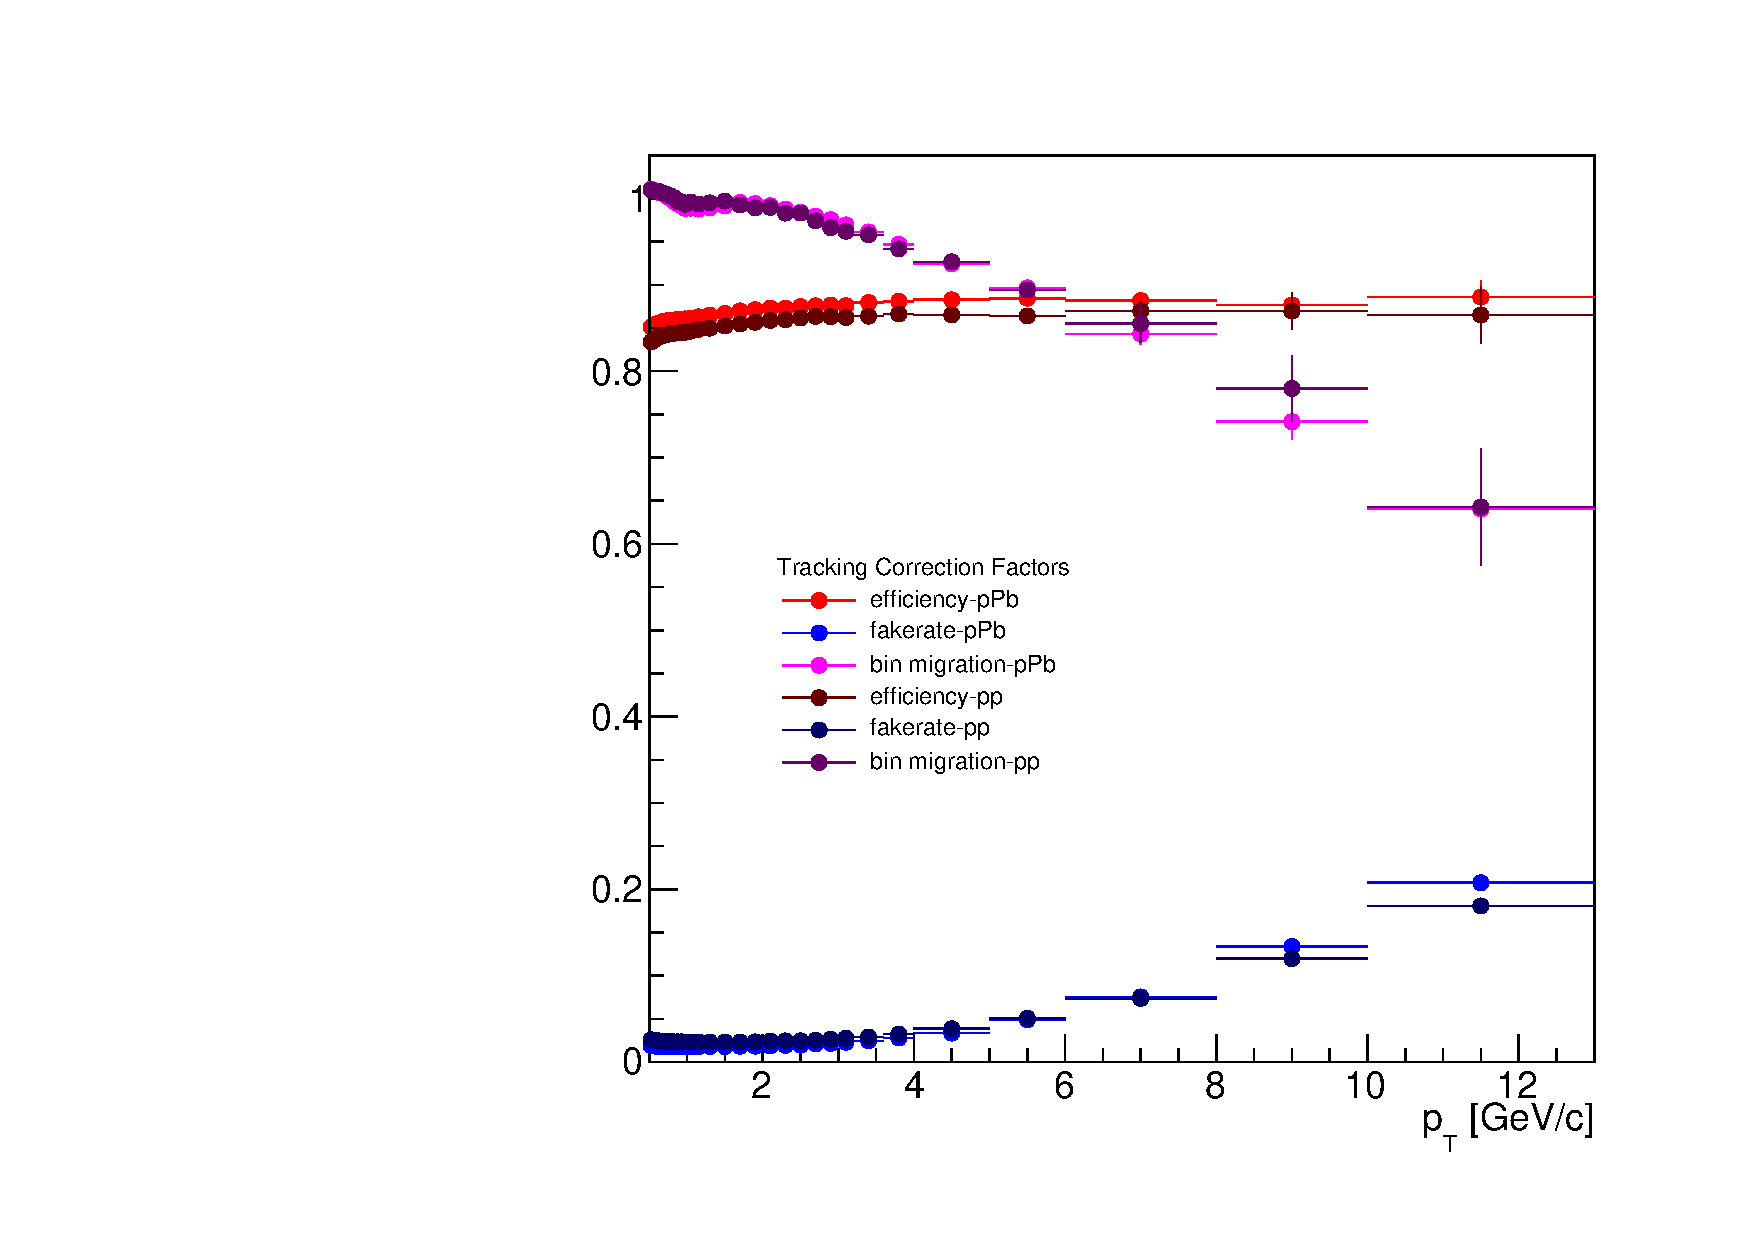
\includegraphics[width=.7\textwidth]{Data_Analysis/Tracking/trackCorrectionFactors_pPbAndpp.pdf}
\caption{The efficiency, fake rate, and momentum smearing correction factors for pp and \pPb~data.}
\label{fig:correctionFactors}
\end{figure}

\FloatBarrier

\subsection{Angular Dependence of Tracking Efficiency}
The 2D $\varphi$-$\eta$ efficiency is calculated in a similar way to the $\pt$ efficiency described in Equation~\ref{eq:eff}, but instead of being functions of $\pt^{\mathrm{true}}$, the efficiency is a function of the true azimuthal angle and pseudorapidity, $\varphi^{\mathrm{true}}$ and $\eta^{\mathrm{true}}$ respectively. Only tracks with {$\pt^{\mathrm{true}}>1$} \GeVc~are considered to avoid tracks with sharp bends in the magnetic field that would obscure the impact of dead regions.

\begin{figure}[h]
\center
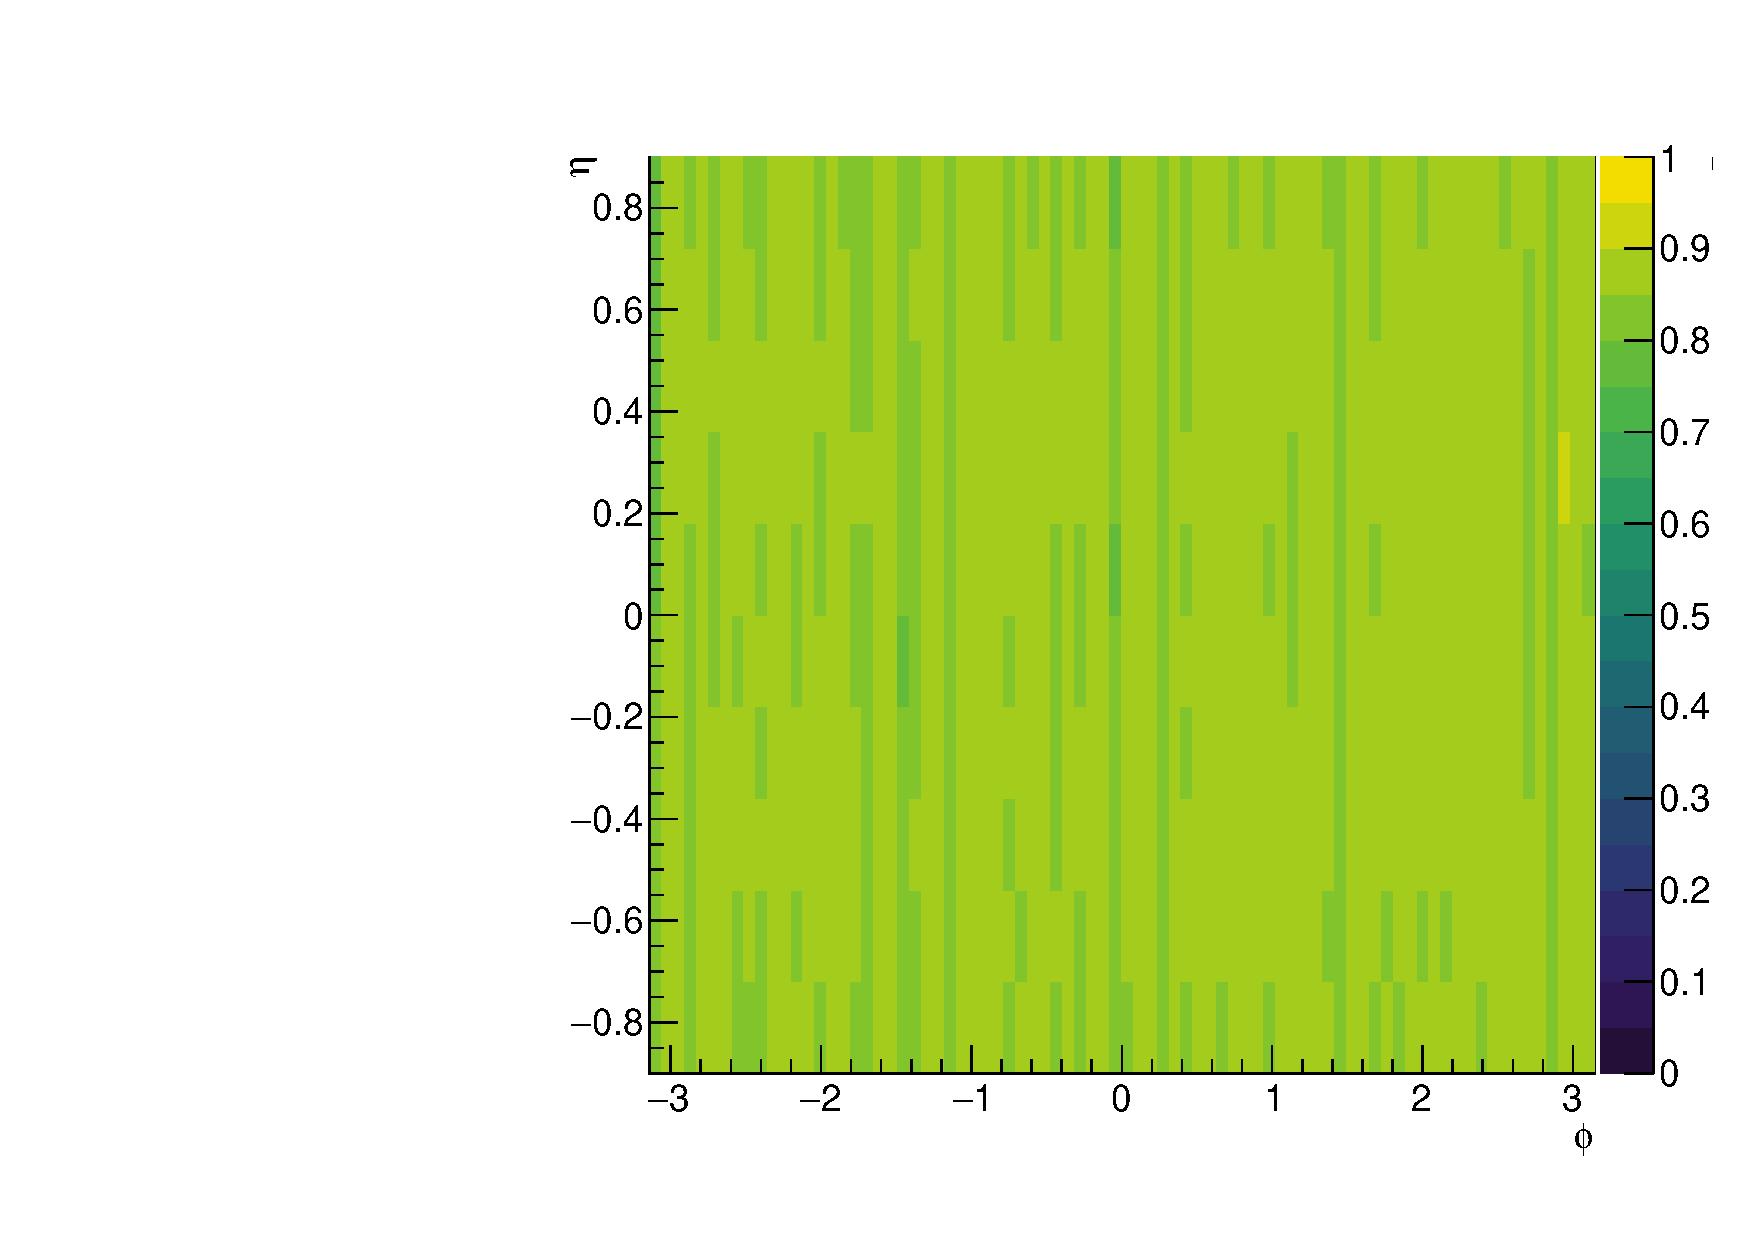
\includegraphics[width=0.46\textwidth]{Data_Analysis/Tracking/etaPhi_eff_tpc.pdf}
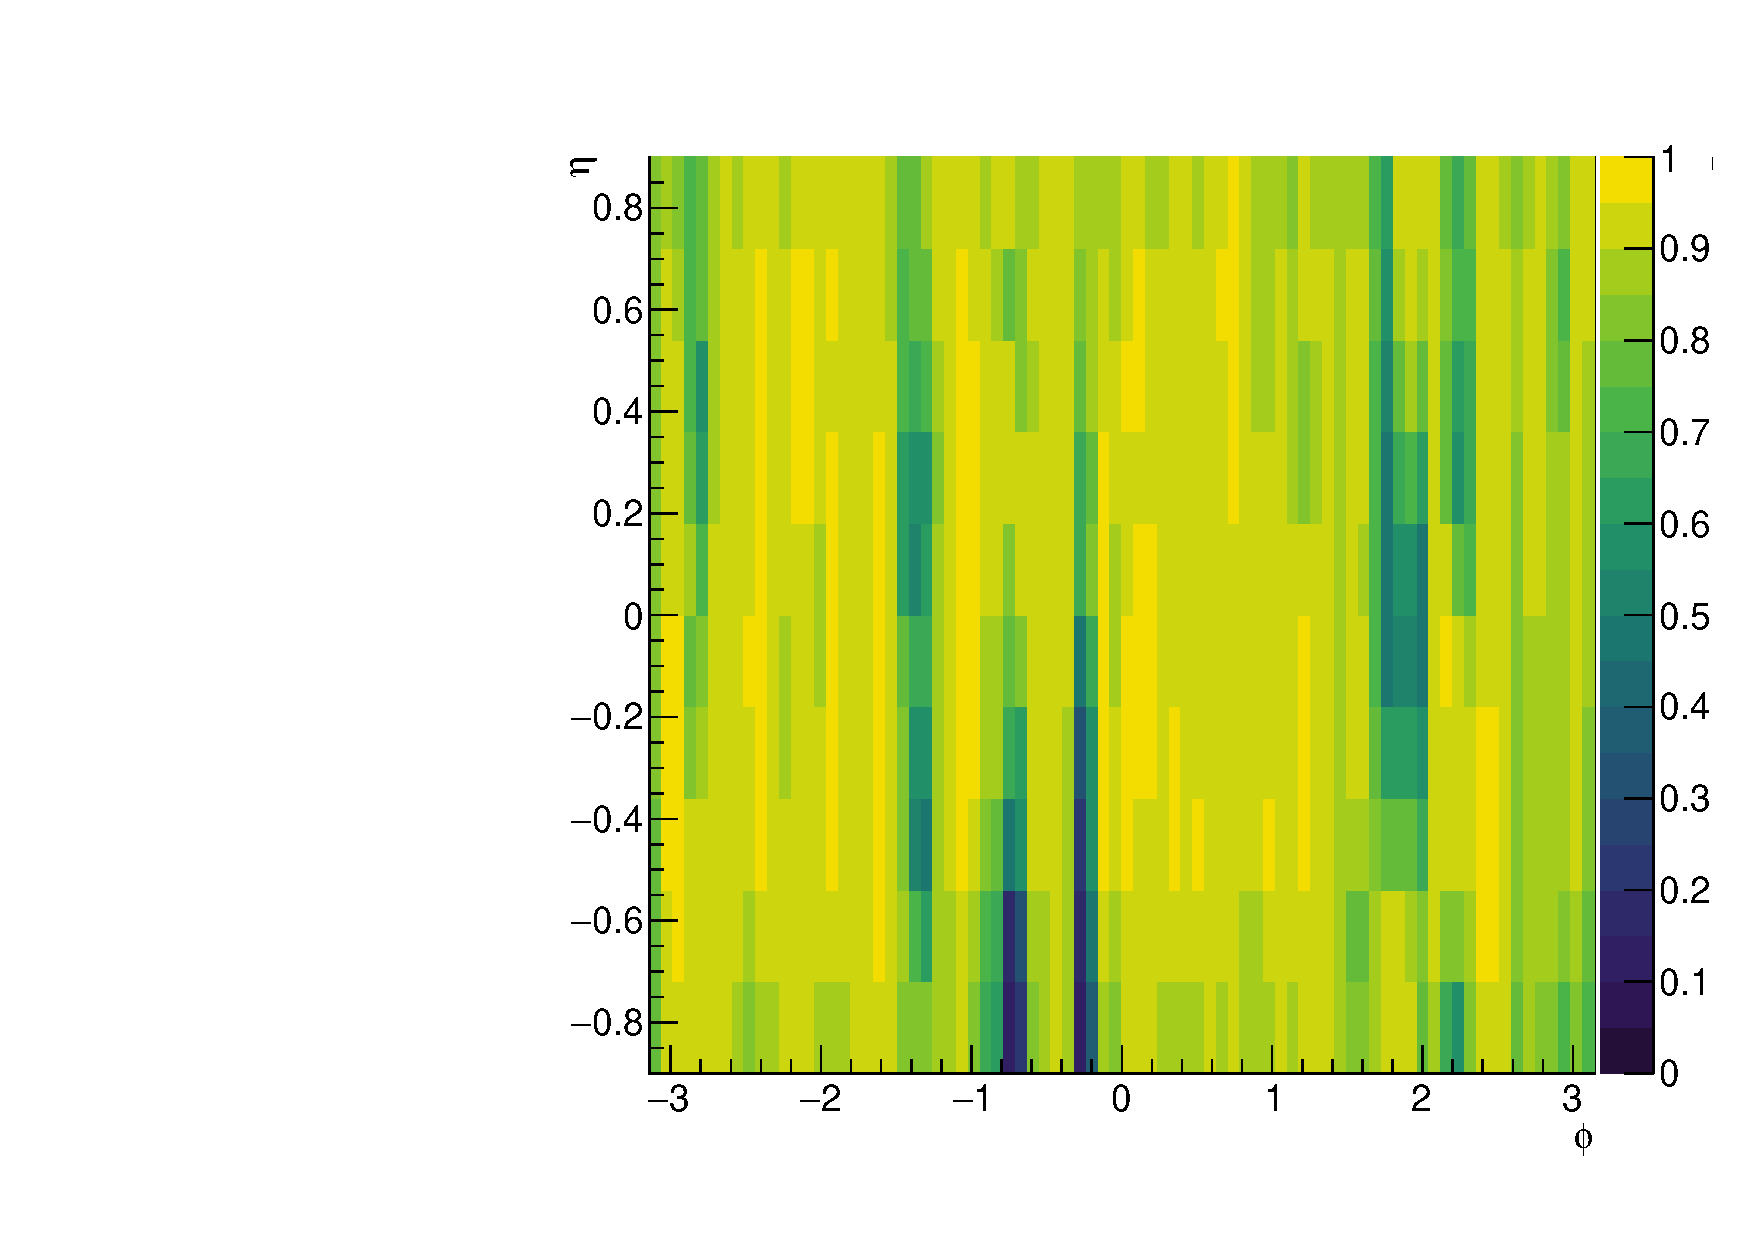
\includegraphics[width=0.46\textwidth]{Data_Analysis/Tracking/etaPhi_eff_4layers.pdf}
\caption{Tracking efficiency as a function of $\varphi^{\mathrm{true}}$ and $\eta^{\mathrm{true}}$ for TPC+ITS (left) and ITS-only (right) tracks.}
\label{fig:2Defficiency}
\end{figure}

Figure~\ref{fig:2Defficiency} shows the resulting efficiency for TPC+ITS and ITS-only tracks. While the TPC+ITS 2D $\varphi$-$\eta$ distribution looks uniform, this is not the case for the ITS-only distribution, which has visible dips in the efficiency at various $\varphi$. The efficiency is close to unity for most of the phase space covered. There are no big $\eta$ variations, but there are large $\varphi$ variations. The efficiency holes at $\varphi$ = $-$0.8 and $-$0.2 are very visible and reach values close to zero. These are attributed to ITS-staves that are completely dead. Any variations in $\varphi$ in the $\gammaiso$-hadron analysis are corrected for using the event mixing technique described in Section \ref{sec:EventMixing}
\FloatBarrier



\section{Photon Hadron Correlations}


In this study, the exact cross section of isolated photons is not the observable, nor is the cross section of charged hadron production in a given event. The quantity of interest is the number partner particles associated with those trigger photons, relating to the leading order picture of back-to-back prompt photon and parton. Therefore, instead of quoting the absolute yield of pairs, it is useful to divide by the number of triggers to obtain the conditional yield (also called per-trigger yield) of associated hadrons. This quantity is typically plotted as a function of the azimuthal angle between the trigger and partner particle, \deltaphi:

\begin{equation}
	\deltaphi \equiv \phi^\mathrm{cluster} - \phi^\mathrm{track}
\end{equation}

 The \deltaphi~distribution of cluster-track pairs, divided by the number of triggers is defined as the trigger normalized correlation function, $C$:

\begin{equation}
\label{eq:basic_correlation}
	C \equiv \frac{P}{T}
\end{equation}

Where $T$ is simply the number of triggers, and $P$ is the \deltaphi~distribution of cluster-track pairs. Such distributions often highlight the structure of jets. They typically contain a large, very narrow peak at $\deltaphi=0$, arising from the autocorrelation of the particles within an jet, and a broader peak centered at $\deltaphi=\pi$ arising from the correlation between two jets in the event, shown in Fig.~\ref{fig:dihadron_cartoon}. 

Enforcing an isolation requirement will heavily suppress the near side peak, however. The near side peak is further removed after the decay photon hadron correlation is subtracted, likely removing the remaining contribution of background jets to the isolated photon triggers \ref{sec:decay_photon_subtraction}. This becomes particularly important for the underlying event estimate detailed in \ref{sec:ue_subtraction_correlations}

%TODO fix ue_subtraction_correlations reference

At lowest order in QCD, prompt photons exactly balance the hard scattered parton in the event. For this reason, studies of photon-tagged jets and jet fragments have been dubbed the "golden channel" for studying parton. %Save for correlations section

%Low energy jets are of particular interest as they are less time dilated, and thus the timescale of fragmentation is comparatively less compared to higher energy jets. By studying jet fragments...

%We actually get an extremely inclusive sample of jets. One needs to make the argument first that jets are a quickly spectrum in pT. If so, then we can only really make an argument on jets around the mean of the distribution.
Eq.~\ref{eq:basic_correlation} is closely related to Eq.~\ref{eq:yield}. The former can be thought of as an ingredient to the latter; Eq.~\ref{eq:basic_correlation} refers to the correlation function over the full range of \deltaphi, while Eq.~\ref{eq:yield} refers to the yields, often the result of integrating $C$ at large  $\deltaphi$.

\subsection{Signal Correlation Function}


%TODO edit this with the equations from the note

\begin{comment}
	In this section we present the method we use to extract \gammaiso-hadron azimuthal correlations. We select tracks with $|\eta|<0.8$ and $0.5 <\pttrack < 10$ \GeVc, following the studies shown in Section~\ref{sec:tracking}. We only consider cluster-track pairs within $|\Delta \eta| < 1.2$. Our cluster \pt~range selection is $12 < \ptcluster< 40\ \GeVc$, with isolation criteria of $\iso < 1.5\ \GeVc$. We apply the same track selection criteria described in Section~\ref{sec:tracking}, Table \ref{tab:track_cuts}. We present our results as a function of \zt, which is defined as:
 \begin{equation}
\zt = \frac{\pttrack}{\ptcluster}
 \end{equation}

Section~\ref{sec:decaybkgsubtraction} shows the way we correct for the impurity of our \gammaiso selection; Section~\ref{sec:EventMixing} describes the pair-acceptance correction obtained with the event-mixing method.


\subsection{$\ydecay$ background Subtraction}
\label{sec:decaybkgsubtraction}
We split the clusters that pass our $\iso<1.5 $ GeV selection in two regions of interest, our signal region \(SR\) with the selection $\lambdasquare<0.3$, and our background region, \(BR\) as $\lambdasquare>0.4$ 

\end{comment}

Section \ref{sec:photons} introduced isolated prompt photons as the primary photon signal for this measurement. However, as detailed in \ref{sec:purity}, there is a substantial amount of background contributing to \gammaiso candidates and a subsequent contribution to the \gammaiso-hadron correlations. In this section, we the disentangle the signal of this measurement from what is initially measured.\\ 

We directly measure the trigger-normalized correlation of shower signal region isolated clusters and associated hadrons, \CSR. This quantity will be made up of the true signal correlation function, \CS~-- the correlation of isolated prompt photons and associated hadrons from the recoiling parton-- as well as the true background correlation, \CB, predominantly arising from the correlation between decay photons that pass the cluster selection and hadrons. We call this background the correlated background, as it arises from the correlation of background photons and the hadrons in the event. To separate what is initially measured, \CSR, and the true signal, \CS, we begin by taking a look at the ingredients of \CSR. First, we denote the number of trigger clusters in the shower signal region, also called the number of \gammaiso candidates, \TSR. We can write \TSR~as:
%TODO Fix reference for shower shape ranges
\begin{equation}
\label{eq:TS_TB}
\TSR = \TS + \TB.
\end{equation}

Here we define \TS~as the number of "true" signal triggers (i.e. the number isolated prompt photon triggers) and \TB~as the background, most prominently decay photons that pass our $\gammaiso$ selection. Similarly, the \deltaphi~distribution of signal region cluster-track pairs, \PSR~ can be written as:
\begin{equation}
\label{eq:PS_PB}
\PSR = \PS + \PB.
\end{equation}

Now, following the notation of Equation \ref{eq:basic_correlation}, we can write the  trigger-normalized correlation functions for shower signal region clusters as:
\begin{eqnarray}
\label{eq:CSR}
\CSR &=& \frac{1}{\TSR}\PSR.
%\CBR &=& \frac{1}{\TBR }\PBR.
\end{eqnarray}
These quantities are directly measured. Similarly, we can write the true signal and true background correlation functions:
\begin{eqnarray}
\CS &=& \frac{1}{\TS}\PS\\\label{eq:CS}
\CB &=& \frac{1}{\TB}\PB\label{eq:CB}
\end{eqnarray}

The goal of this formalism is to write the true signal correlation function (\CS)~in terms of quantities that are measured --  \CSR~and the measured purity, $p$. To this end, the next step is to write the measured quantity, \CSR, in terms of true signal and true background correlation functions:
 
\begin{eqnarray}
\label{eq:31}
\CSR &=& \frac{1}{\TSR}\PSR = \frac{1}{\TSR}(\PS + \PB)\\
\CSR &=& \frac{1}{\TSR}(\TS\CS +\TB\CB)\label{eq:CSR_TS_TB}
\end{eqnarray}

Where we have substituted equation \ref{eq:PS_PB} into  Equation \ref{eq:CSR}, followed by using Equations \ref{eq:CS} and \ref{eq:CB} to substitute out \PS~and \PB, respectively. \TS~ and \TB~ are not directly measured, however they can be expressed in terms of measurable quantities. The purity is defined as the fraction of true signal in our \gammaiso clusters, or in other words, $p \equiv \TS/\TSR$~(see Section~\ref{sec:purity}). Substituting this into equation \ref{eq:TS_TB} and solving solving for \TB/\TSR, one obtains: $\TB/\TSR = 1-p$. This a natural result of the definition of purity: If $p$ is the fraction of the true signal making up the \gammaiso candidates, $1-p$ must be everything else, i.e. background. To summarize:

\begin{eqnarray}
	p &\equiv & \TS/\TSR\\
	1-p &=& \TB/\TBR
\end{eqnarray}


Substituting $p$ into Equation \ref{eq:CSR_TS_TB}:
\begin{equation}
	\CSR = p\CS+ (1-p)\CB \label{eq:CSR_CS}
\end{equation}

Finally, we can solve for \CS~in terms of \CSR~and $p$:
\begin{equation}
\CS = \frac{\CSR - (1-p) \CB}{p}
\label{eq:FinalSubtraction_CB}
\end{equation}


Equation \ref{eq:FinalSubtraction_CB} shows \CS~in terms of the measured quantities, \CSR~and the purity. It also includes, however, a term for the background correlation function \CB, that cannot be determined from \CSR and the purity alone. The correlation function \CB is described in more detail in section \ref{sec:cb}.

\subsection{Decay Photon Hadron Correlations}
\label{sec:cb}

There is a large fraction of \ydecay background within the isolated photon sample, and a subsequent $\gamma^\mathrm{decay}$-hadron correlation present in the measured correlation function. The correlation between hadrons and background photons within the \gammaiso sample, most prominently photons from neutral meson decays, correspond to the \CB~term in in Equation \ref{eq:FinalSubtraction_CB}. While the equation gives us the scale of this background, $1-p$, it does not offer information on the shape of this \deltaphi distribution. To understand the shape, we take advantage of the fact that the most prominent source background photons within the \gammaiso population are photons from neutral meson decays. Outside of the \gammaiso selection, these photons tend to have more assymmetric shower profiles, and thus larger values of \lambdasquare. Therefore, in order to select on clusters arising from decay photons, an inverse shower shape selection is applied which we define as the shower background region, BR:

\begin{equation}
	\label{eq:BR}
	\lambdasquare(\mathrm{BR}) > 0.4
\end{equation}

Thus, in order to approximate \CB, a \ydecay hadron correlation function is measured by taking the correlation of clusters in the shower background regions with associated hadrons in the event. This shower background region correlation function, much like Eq. \ref{eq:CSR} is defined as \CBR:
\begin{equation}
\CBR = \frac{1}{\TBR}\PBR.
\end{equation}

With \TBR as the number of clusters in the shower background region, and \PBR~as the \deltaphi~distribution of shower background region clusters and hadrons.\\

Notably, because the underlying physics process that dictates the number and distribution of correlated pairs is independent of the opening angle of the neutral-meson decay, which is what drives the shower-shape, the approximation $\CBR \approx \CB$ can be made.\footnote{Here again we take advantage of trigger normalized quantities. The number of isolated photons in the shower background region vastly outnumber the number of isolated photons within the shower signal region. By focusing on the associated yield of hadrons per each photon, which is not correlated with \lambdasquare, this very useful approximation can be made.} In other words, the shower background region correlation function is a good approximation of the correlated background that contributes to the shower signal region correlation function, \CSR. Therefore, Eq. \ref{eq:FinalSubtraction_CB} can be re-written:
\begin{equation}
\CS = \frac{\CSR - (1-p) \CBR}{p}
\label{eq:FinalSubtraction}
\end{equation}

As a result, the true signal correlation function, \CS, is finally written in terms of measurable quantities: The shower signal region correlation function, \CSR, the purity, p, and the newly defined shower background region correlation function (or \ydecay correlation), \CBR.

Thus, hadrons are correlated with clusters in the shower background region to directly measure the \ydecay-hadron correlation functions. This \ydecay-hadron correlation function is then subtracted from the the shower signal region correlation function to obtain the signal correlation. This scaling, however, must be done carefully due to the \pt~dependance of the purity. The next few sections describe corrections to the correlation functions. Unless explicitly stated, these corrections (purity weighting, acceptance corrections, and charged particle tracking corrections) are applied to both the \CSR and \CBR before the two are finally subtracted in Sec.~\ref{sec:decaybkgsubtraction}


%where we have made the approximation that \CB~ (per-trigger pairs for decay photons that pass our $\gammaiso$ selection) can be approximated by the measured \CBR~(per-trigger pairs for decay photons that pass our isolation criteria but not our shower-shape selection). This is justified because the underlying physics process that dictates the number of correlated pairs is independent from the opening angle of the neutral-meson decay, which is what drives the shower-shape.
       
%This scaling, however, must be done carefully due to the \pt dependance of the purity

%TODO Final subtraction error propagation. Articulate the point that CSR and CBR are calculated independantly
%TODO include gaussion error propagation calculation. Point out that this overestimates the uncertainty, as there is a clear correlation in applynig the purity to CBR and CSR. Show what's done instead.


%The correlated background subtraction detailed in Equation~\ref{eq:FinalSubtraction} assumes that the decay-photon hadron correlation we directly measure, \CBR, is an accurate estimation of the decay-photon hadron correlation that pollutes signal region. In principle, the decay photons from neutral-meson decays that pass the shower shape cut may be biased toward pairs with a smaller opening angle (larger cluster \pt). We checked this by forcing the \pt distributions in \CSR and \CBR. 


\subsection{Photon Purity Weighting}

%The \ydecay-hadron correlations is scaled according to the purity, in this case $1-p$ and subtracted. %With the purity quantifying the fraction of true signal present in \gammaiso candidates, $1-p$ indicates the fraction of background.
Equation \ref{eq:FinalSubtraction} shows the background correlation function, \CB, approximated by the \ydecay~correlation function, and scaled by $1-p$ according to its relative contribution measured correlation function. The purity is a \pt dependent quantity, rising quickly with \pt, correlations using a low-\pt~cluster have a higher fraction of background than high-\pt~clusters (see Figure \ref{fig:purity}). As a result, measuring the \ydecay-hadron correlation function for all clusters and scaling by the mean of the purity would lead to and underestimation of the background at low \ptcluster, and an overestimation at high \ptcluster. This has will have a non-trivial effect on the corresponding \zt~bins, which include clusters with a wide range of \ptcluster. Additionally,  Equation \ref{eq:FinalSubtraction} includes an overall scale of 1/$p$ in order to obtain the correct conditional yield of hadrons after the subtraction in the numerator, and will yield similar complications if applied correlations using clusters over the full \ptcluster~ range.\\

In order to avoid these complications, clusters are weighted by the purity corresponding to their exact \ptcluster~when constructing the correlation functions. In order to capture the quickly rising behavior of the purity at low \ptcluster, the purity is fit to a 3-parameter error function. This fit to the purity is shown in Figure \ref{fig:Purity_Error_Function}The \ptcluster becomes an input to this function, and precise purity weighting is applied precisely to each cluster. 

\begin{figure}
	\label{fig:Purity_Error_Function}
	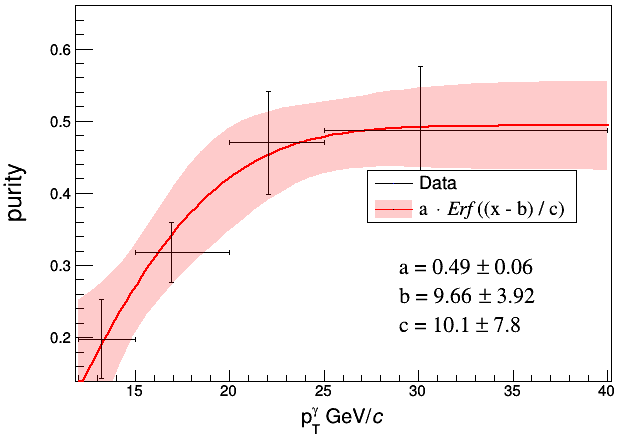
\includegraphics[width=0.5\textwidth]{Data_Analysis/Error_Function_Fits/pp_Mean_Center}
	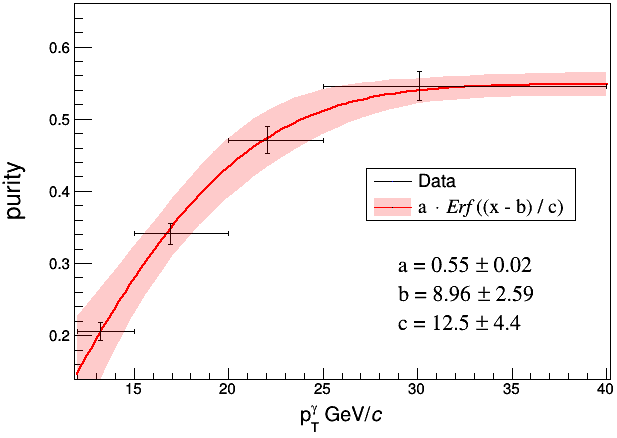
\includegraphics[width=0.5\textwidth]{Data_Analysis/Error_Function_Fits/pPb_Mean_Centers}
  \caption{A 3-parameter error function is fit to the purity values measured in pp (left) and \pPb~(right) data. The width of the band represents the uncertainty on the fit.}
\end{figure}


According to Equation \ref{eq:FinalSubtraction}, the overall purity weights will be $1/p$ and $(1-p)/p$ for shower signal and shower background region clusters, respectively. 

\subsection{Track Efficiency, Fake Rate, and Bin Migration Weights}
In order to correct for the tracking efficiency, fake rate, and bin-migration we apply a track-by-track weighting according to:

\begin{equation}
w_{\mathrm{tracking}}(\pt^{\mathrm{track}}) = \frac{1}{\epsilon}\times(1- f)\times b.
\end{equation}

Here $\epsilon$ is the track efficiency, $f$ is the fake rate, and $b$ is the bin-to-bin migration correction. These are described in Section~\ref{sec:tracking}. The corrections are estimated independently for pp and \pPb~data although the performance is very similar. The weights are applied to the measure charged hadrons as the correlation functions are being constructed, analogous to how the purity weighting is applied to the photons in the correlations functions.

\subsection{Pair-Acceptance Correction with Event Mixing}

\label{sec:EventMixing}
%TODO: Add reference to detector setup, and point out the acceptance of EMCal and ITS
Initially, two particle correlations consist of a combination of true physical correlations and detector effects. The detector effects result from inefficiencies and limited acceptance in the detectors. The study of trigger normalized yields of associated hadrons eliminates the need to correct for isolated cluster efficiency, and Section \ref{sec:tracking} outlines the charged tracking efficiency correction. %TODO: Fix Tracking Reference.

The remaining detector effect on the correlations are pair-acceptance effects:
correlations are constructed through pairs of clusters and charged tracks. This results in a convolution of acceptance effects from the limited acceptance of EMCal and ITS, which we call pair acceptance effects. These effects are corrected for by using the event mixing technique. Event mixing is a data driven approach to correcting for detector acceptance effects \footnote{Event mixing is also used for estimating combinatorial background.}. By constructing observables with particles from different events, we remove true physics correlations from the correlation functions, isolating detector effects from limited acceptance in \(\eta\) and detector inhomogeneity in $\eta$ and $\varphi$. 


Cluster-track pairs in same event correlation functions obviously share the properties of the event, and such properties often effect detector response. In order to make the mixed-event correlations as analogous as possible to the to same-event correlation functions, events that are as similar as possible with respect to these event properties are used for event mixing. The two most important event properties for this measurement are multiplicity and the z-coordinate of the reconstructed primary vertex (i.e. the position of the primary interaction vertex along the beam direction)\footnote{In Lead-Lead collisions, the event-plane angle which determines the anisotropic distribution of final state particles, or $v_{2}$, is also one of the most important event properties to match in Event mixing. However, because this measurement focuses on smaller systems, pp and \pPb, this effect can be neglected}. %Thus, events that are that are very similar in multiplicity and z-vertex are matched together.\\



%TODO Explain Mp and Vz
 
 The goal of event mixing is to isolate detector effects by completely removing true physics correlations. To this end, $\gamma$-triggered events are not mixed with other $\gamma$-triggered events. Triggering on a high \pt photon will result in an enhancement of away-side hadrons due to the recoiling jet. Due to the limited acceptance of the EMCal, this enhancement will be concentrated in a small area of the ITS, approximately 180$^{\circ}$ opposite the EMCal trigger. Mixing only with triggered events will result in a "pseudo" recoiling jet signal that would be suppress the true signal in the same-event correlation function when the event mixing correction is applied. Instead, $\gamma$-triggered events are mixed with minimum bias events to avoid this bias, and to sample the full acceptance of the ITS properly.
 
% This is because of the relatively small acceptance of the EMCal trigger, and a resulting enhancement of charged tracks roughly 180\degree arising from the recoiling parton opposite the trigger photon.
 
 %Triggering on a high pT photon will have an enhancement of away-side hadrons due to the recoiling jet. Due to the limited acceptance of the EMCal, using triggered events will result in an enhancement of photons in a specific eta-phi range, as well as an enhancement of hadrons in a specific eta-phi range roughly, both 180° apart in phi for the reason just mentioned. This will distort the Mixed event correlation function by including “fake” recoiling jet signal (fake because the cluster and tracks are obviously from different events). Tracks from minimum bias are chosen to mix with clusters from triggered data to avoid this, i.e. remove any trace of physical correlations.

 
 %In order for the mixed event distribution to reflect background instead of emulating  signal, as well as to fully cover the detector acceptance,
 %we paired each \(\gamma\)-triggered event with minimum bias events. %Subsequent batches of 200 minimum bias events are used, as necessary, to reach the desired number of mixed events per true event. 

For this analysis, depending on the \zt~bin, each \(\gamma\)-triggered event was mixed with up to 300 minimum-bias events.

 Traditionally, events are often placed into bins of multiplicity (V0 amplitude, sum of V0A and V0C) and primary vertex $z$-position, and then mixed within these bins. This has the advantage of conceptual simplicity, but is not very efficient and requires a large amount of cpu time. Instead of bins, the mixing in this analysis is carried out by using a stable matching algorithm~\cite{GaleShapley:1962amm}. Generally, this algorithm is used to pair two sets of populations, where members from both populations have a well defined and ordered preference list. Here, the two populations are $\gamma$-triggered and minimum bias events. The use of this algorithm avoids the need for binning in multiplicity and primary vertex, and is much faster than the standard binning method.
 
The stable matching algorithm first creates a preference list made up of all other events based on how close events are in multiplicity and $z$-vertex. After each event has a preference list, the algorithm loops over all events, with a nested loop that iterates over each event's preference list. The algorithm then pairs  pairs the current event to the first unpaired event on that list. As the loop iterates, if an event towards the end of the main loop has an already-paired event high on it’s preference list, the algorithm loops through the already-paired event's preference list and decides if the paired event should stay paired to its current match, or switch to the new event. If the latter is chosen, the previously matched event is “unpaired” and added back into the loop. A stable state is met when all paired events have a match that is higher on their preference list than any remaining unpaired events in the loop. Such a stable state is guaranteed to eventually be met according to Ref.~\cite{GaleShapley:1962amm}.\\

The pseudo code below follows this description, using \(\gamma\) to denote a \(\gamma\)-triggered event, and \(M_B\) to denote a minimum-bias event. The \textit{unrequested} state refers to a \(M_B\) event on a \(\gamma\)-event's preference list that has not yet been requested for pairing.\\

\FloatBarrier
\begin{algorithmic}
\Procedure{GaleShapleyPairing}{}
\While{\(\exists\) \textit{free} \(\gamma\) with an unrequested \(M_B\) on \(\gamma\)'s list}
\State \(M_B\) = first unrequested MinBias Event on \(\gamma\)'s list.
\If {\(M_B\) is free}
\State (\(\gamma\),\(M_B\)) become paired
\Else{ some pair (\(\gamma\)',\(M_B\)) exists}%
	\If{\(M_B\) prefers \(\gamma\) to \(\gamma\)'}
    \State \(\gamma\)' becomes free
    \State (\(\gamma\),\(M_B\)) become paired
    \Else
    \State (\(\gamma\)',\(M_B\)) remain paired
    \EndIf
\EndIf
\EndWhile
\EndProcedure
\end{algorithmic}

\begin{figure}[h]
\center
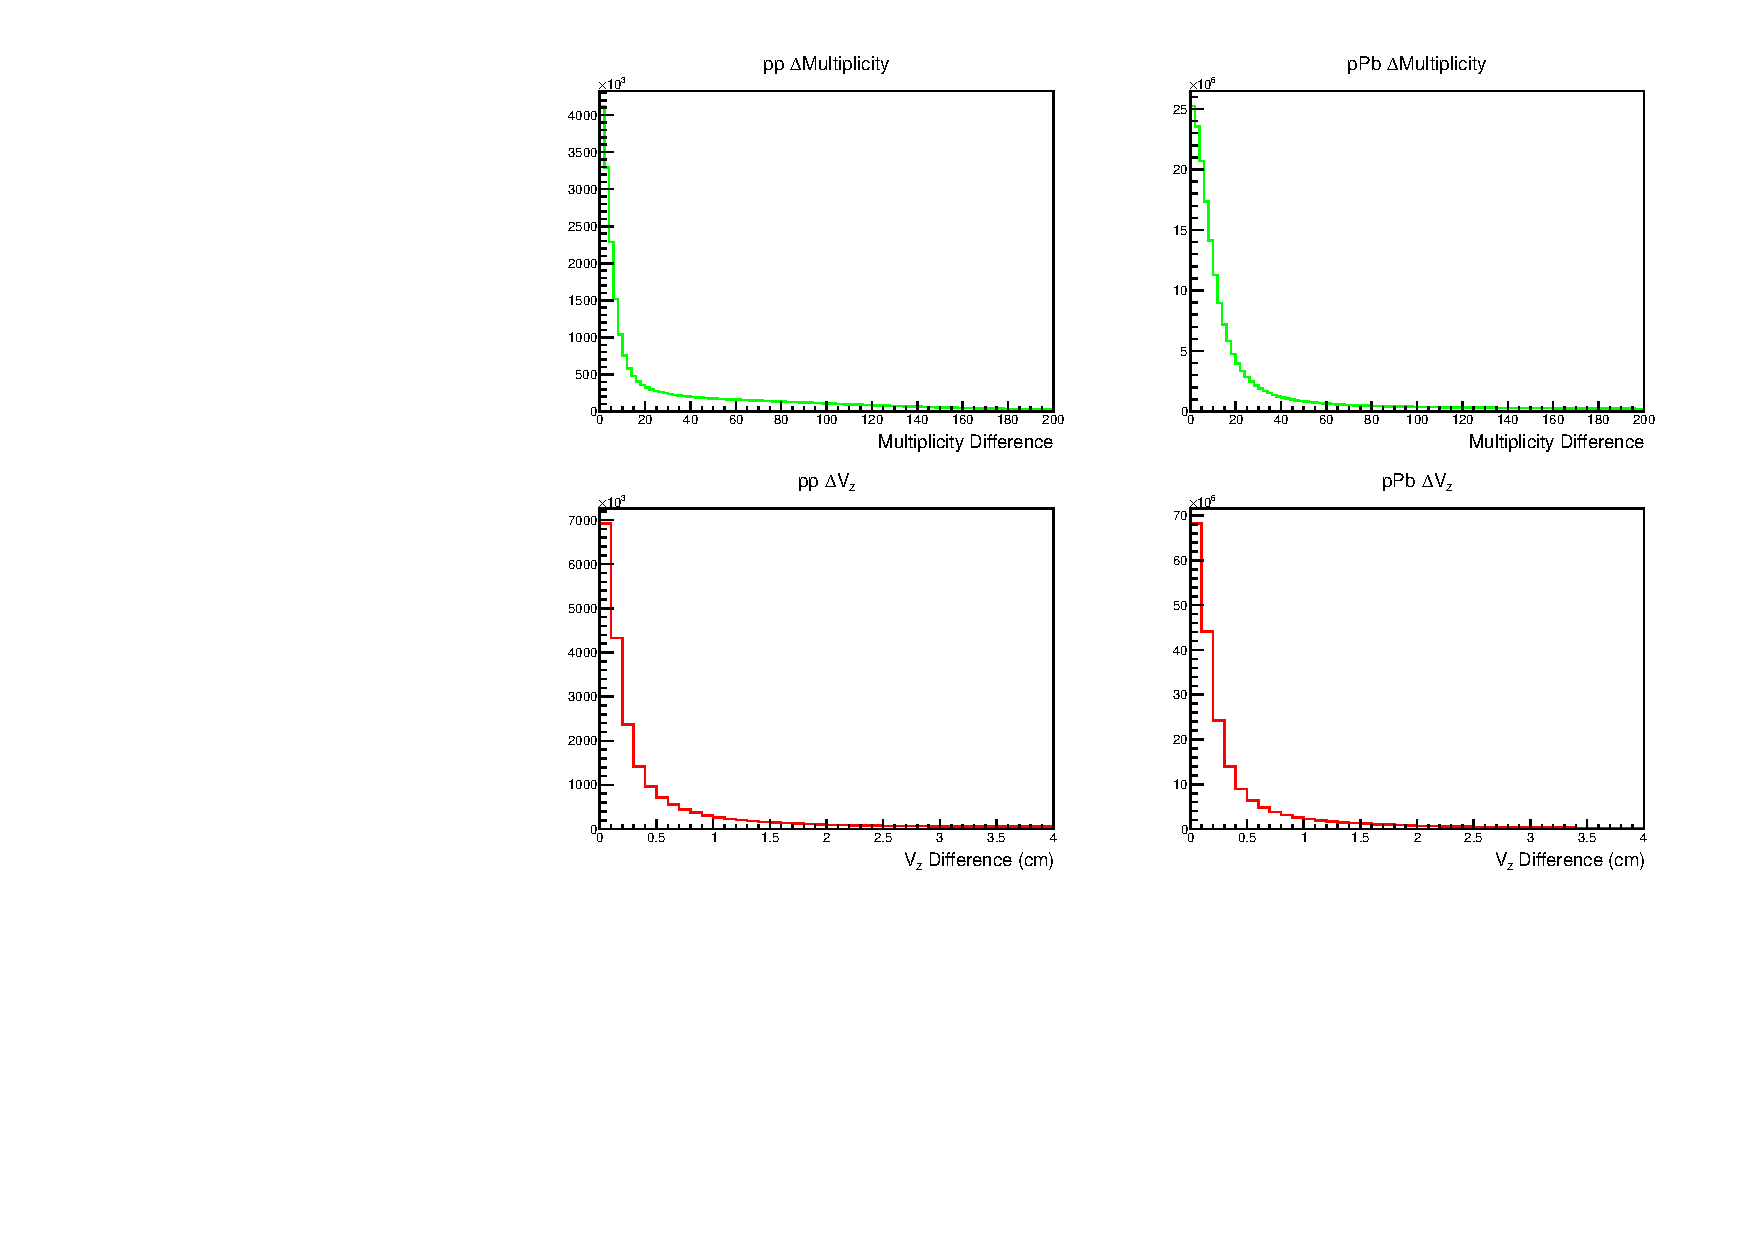
\includegraphics[width=0.95\textwidth]{Data_Analysis/EventMixing/pPb_Differences.pdf}
\caption{Difference in V0 multiplicity
(upper row) and longitudinal vertex position (bottom row) between paired events in pp (left column) and \pPb~right. The pairing algorithm results in sharp peak near zero for these difference distributions, particularly in the longitudinal vertex difference. As described in the text, in the correlation analysis we apply a further selection to cut the large tails observed in these distributions. }
\label{Difference_distributions}
\end{figure}

The difference distributions for Z-vertex and multiplicity between a \(\gamma\)-triggerd and minimum bias events in \pPb~data are shown in Figure \ref{Difference_distributions}. The resulting distributions show a sharp peak that is below {$\Delta z<0.5$ cm} and also a long tail. Less than 6 \% of the distribution lies beyond $\Delta z > 2$ cm. The multiplicity difference, however, does not have as sharp a peak near \(\Delta\)Multiplicity = 0. About 20$\%$ of pairs have a multiplicity difference above 40, and cuts at \(\Delta V_z > 2\)cm and \(\Delta\)Multiplicity \(> 40\) were applied to pairs before calculating correlation functions as a precaution.
%In \pPb events, there was initially a long tail towards larger values of deltaM, however a cut was applied after the pairing procedure to eliminate events that were too Different in Mp or zV.
 Skimming \pPb events with particularly high multiplicities before pairing had a similar effect on the tail of the distribution. However, both skimming events before pairing and applying the previously mentioned cuts after the pairing process had no observable effect on the mixed-event correlation.


Figure~\ref{fig:Multiplicitydistributions} shows the V0 multiplicity distributions for pp and \pPb~data in $\gamma$--triggered events. This shows that a multiplicity matching requirement of \(\Delta\)Multiplicity \(< 40\) is indeed very tight. 

\begin{figure}[h]
\center
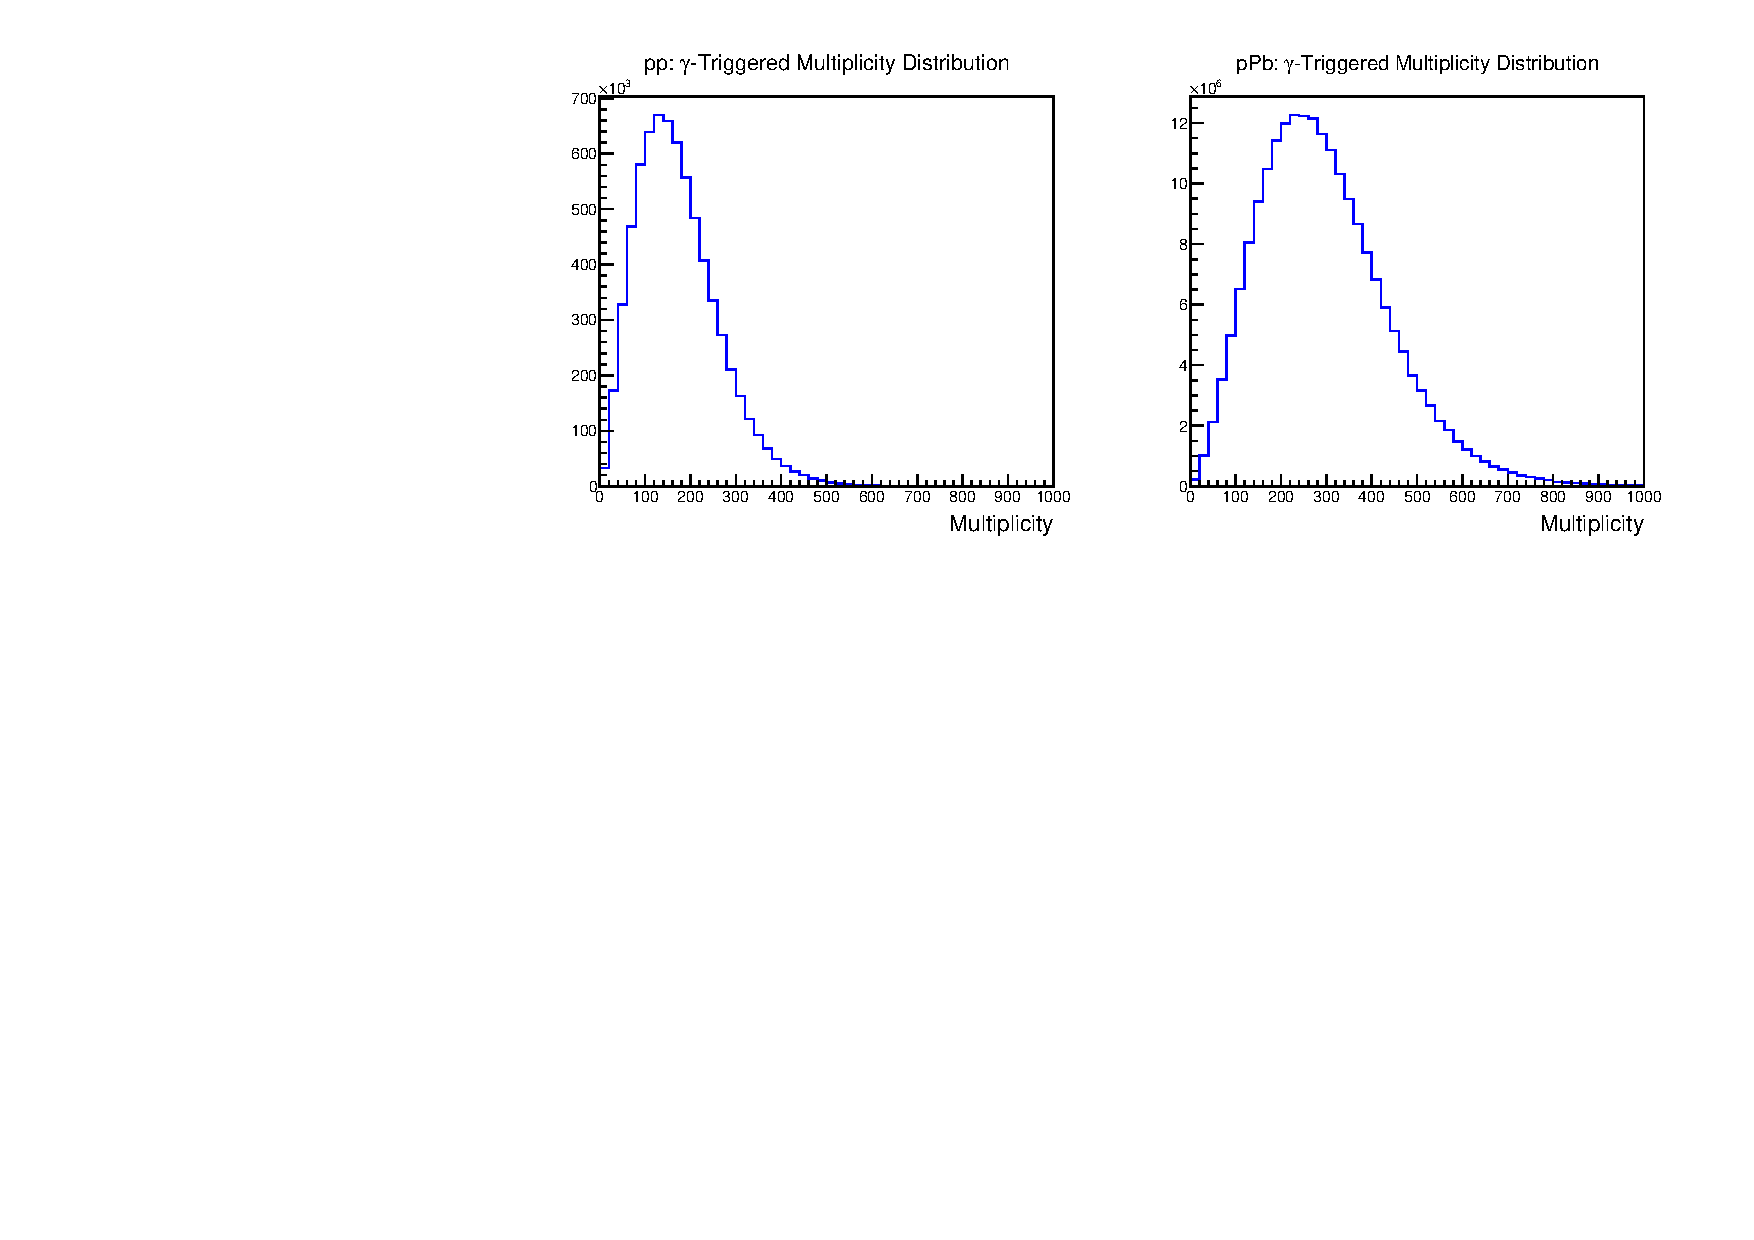
\includegraphics[width=0.9\textwidth]{Data_Analysis/EventMixing/Abs_Multplicity_Dist.pdf}
\caption{V0 multiplicity distribution, i.e. the sum of V0A and V0C amplitudes , in pp (left) and \pPb~(right) gamma-triggered data.}
\label{fig:Multiplicitydistributions}
\end{figure}

Ideally, the mixed event distribution should be flat in \(\Delta\varphi\) and have a trapezoidal shape in \(\Delta\eta\), because the limited acceptance in \(\eta\) increases the likelihood to reconstruct pairs with a small \(\Delta\eta\) (i.e, due to the convolution of two uniformly distributed functions). However, the use of ITS-only tracks and holes in the ITS acceptance result in deviations from a flat distribution in \(\Delta\varphi\). %This is visible in Figure~\ref{GS_Mixed_2D}.

%The highest efficiency to find pairs between the ITS and EMCal should be equal to unity. Thus, the normalization was chosen such that the maximum value of the correction is equal to unity. 
The correlation function corrected by pair-acceptance effects is then given by:
\begin{equation}
\label{eq:Y}
C(\Delta \varphi, \Delta \eta) = \frac{S(\Delta \varphi, \Delta \eta)}{M(\Delta \varphi, \Delta \eta)},
\end{equation}
%TODO Change Mixing Equations to have consistent notation with previous sections
%TODO Add sentence on skimming multiplicity before delta-distributions were made in pPb


%In \pPb events, there was initially a long tail towards larger values of deltaM, however a cut was applied after the pairing procedure to eliminate events that were too Different in Mp or zV. Skimming events events with particularly high multiplicities before pairing had a similar effect on the tail of the distribution. However, both skimming events before applying the algorithm and applying this cut afterward had a negligible effect on the final mixed event correlations.

where $S(\Delta \varphi, \Delta \eta)$ is the same-event correlation, and $M(\Delta \phi, \Delta \eta)$ is the mixed-event correlation. $S(\Delta \phi, \Delta \eta)$ is given by: 
\begin{equation}
S(\Delta \varphi, \Delta \eta) = \frac{1}{N_{\mathrm{trig}}}\frac{d^2N_{\mathrm{same}}}{d\Delta \varphi d\Delta \eta}
\end{equation}

With \Ntrig~as the number of trigger particles and \Nsame~as the number of same event cluster-track pairs and $d^2\Nsame/d\Delta \varphi d\Delta \eta$ is found by pairing trigger particles with tracks from the same event. The mixed-event distribution, $M(\Delta \varphi, \Delta \eta)$, is given by 
\begin{equation}
M(\Delta \varphi, \Delta \eta) = \alpha \frac{d^2 \Nmixed}{d\Delta \varphi d\Delta \eta}.
\end{equation}

Where $\alpha$ is the normalization constant that sets the maximum value of the mixed event correlation to 1, and \Nmixed~is the number of mixed event cluster-track pairs. The term $d^2 \Nmixed/d\Delta \varphi d\Delta \eta$ is obtained by pairing trigger particles from \(\gamma\)-triggered events with tracks from minimum bias events matched in z-vertex and multiplicity.


\begin{figure}
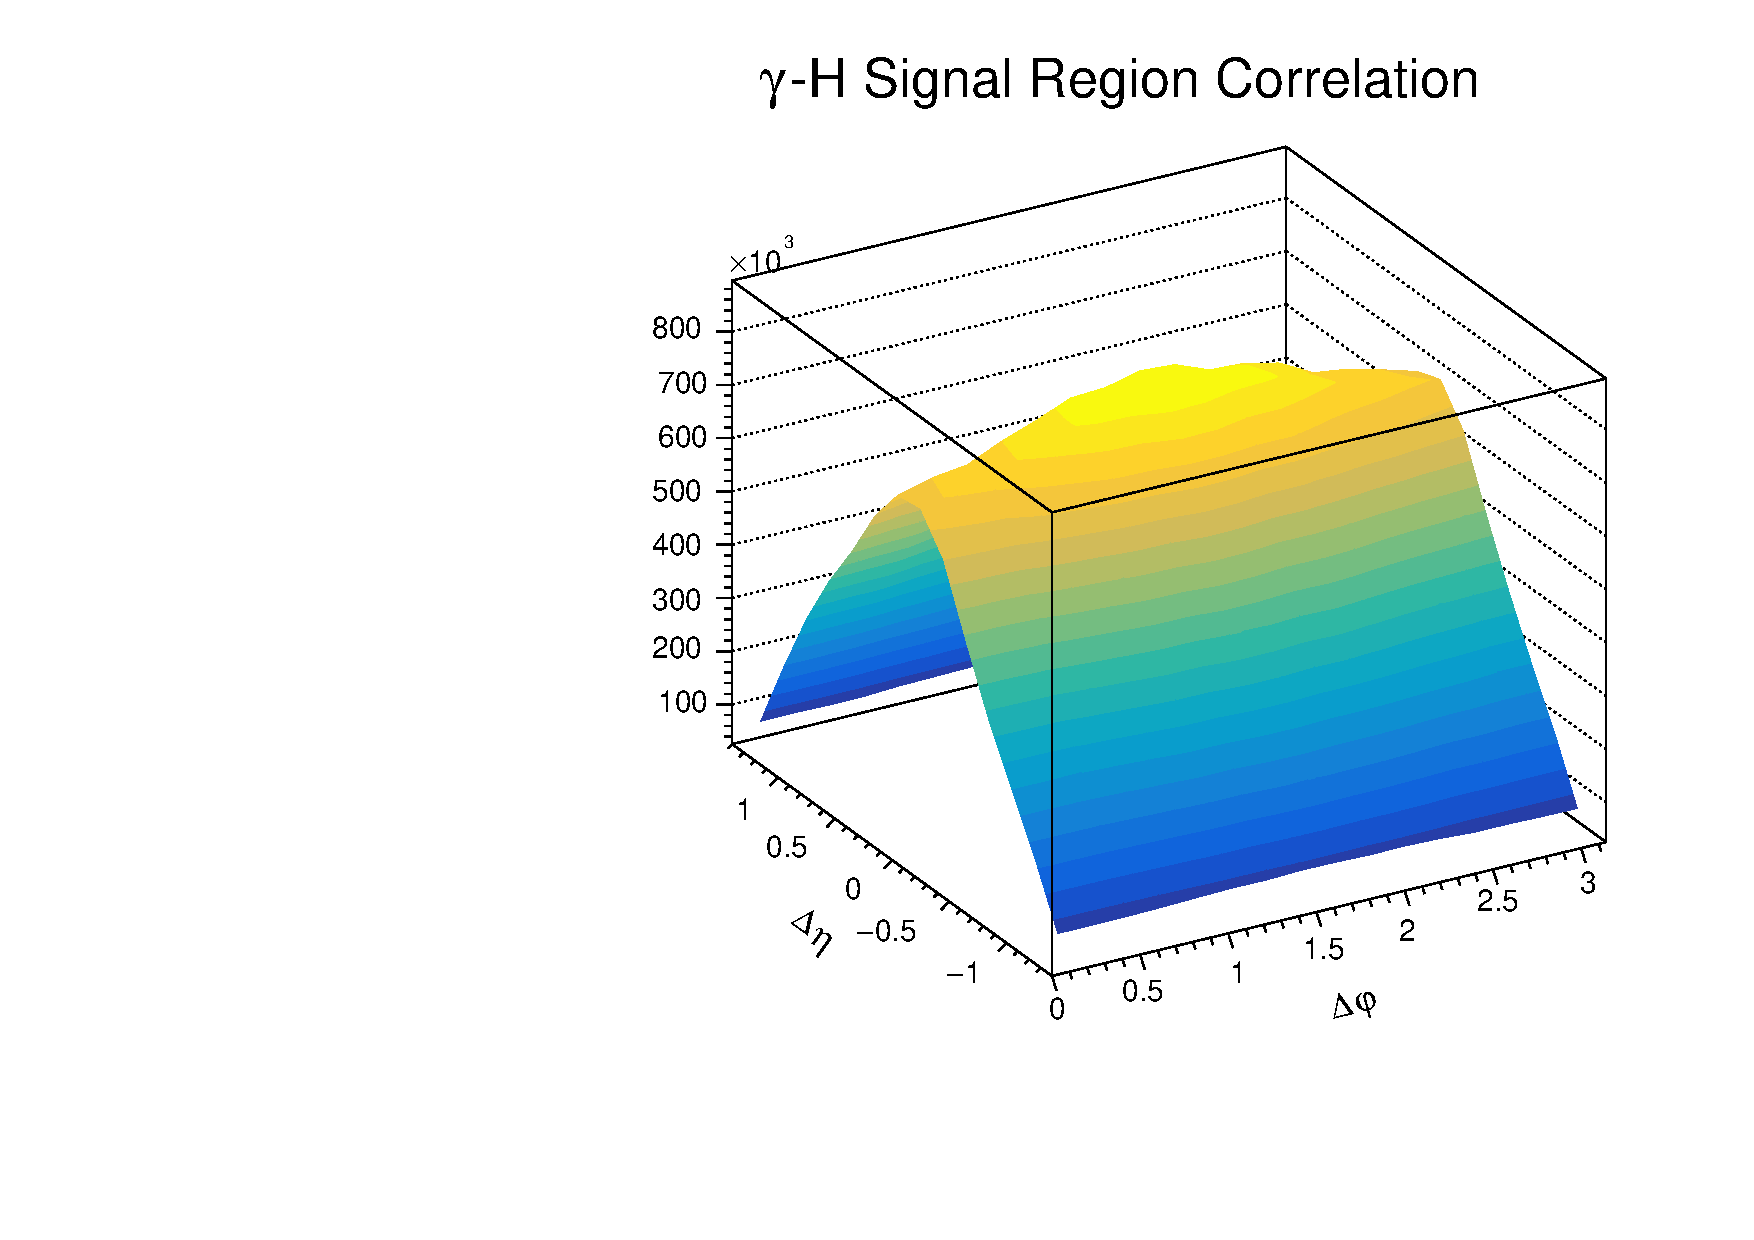
\includegraphics[width=0.32\textwidth]{Data_Analysis/G-H_New/2D_SR_ME.pdf}
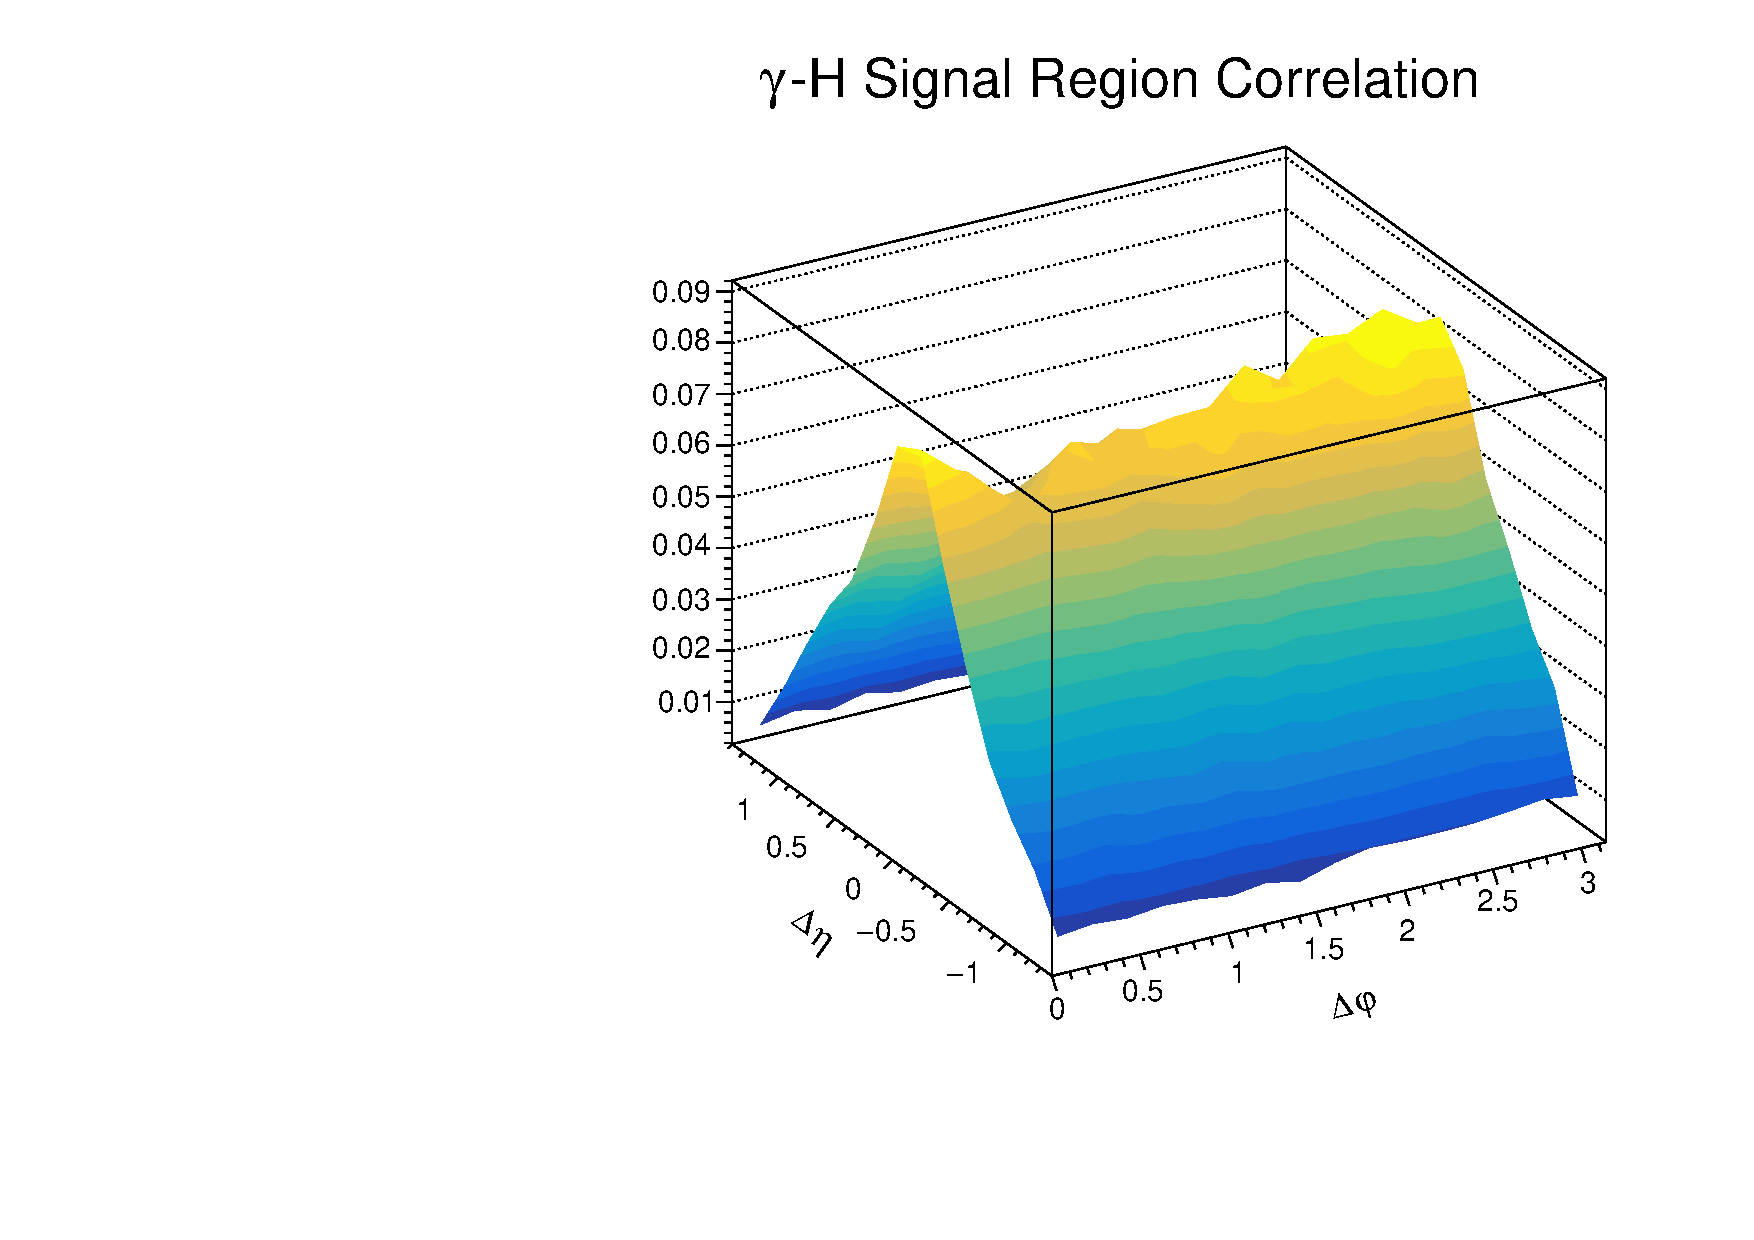
\includegraphics[width=0.32\textwidth]{Data_Analysis/G-H_New/2D_SR_SE.pdf}
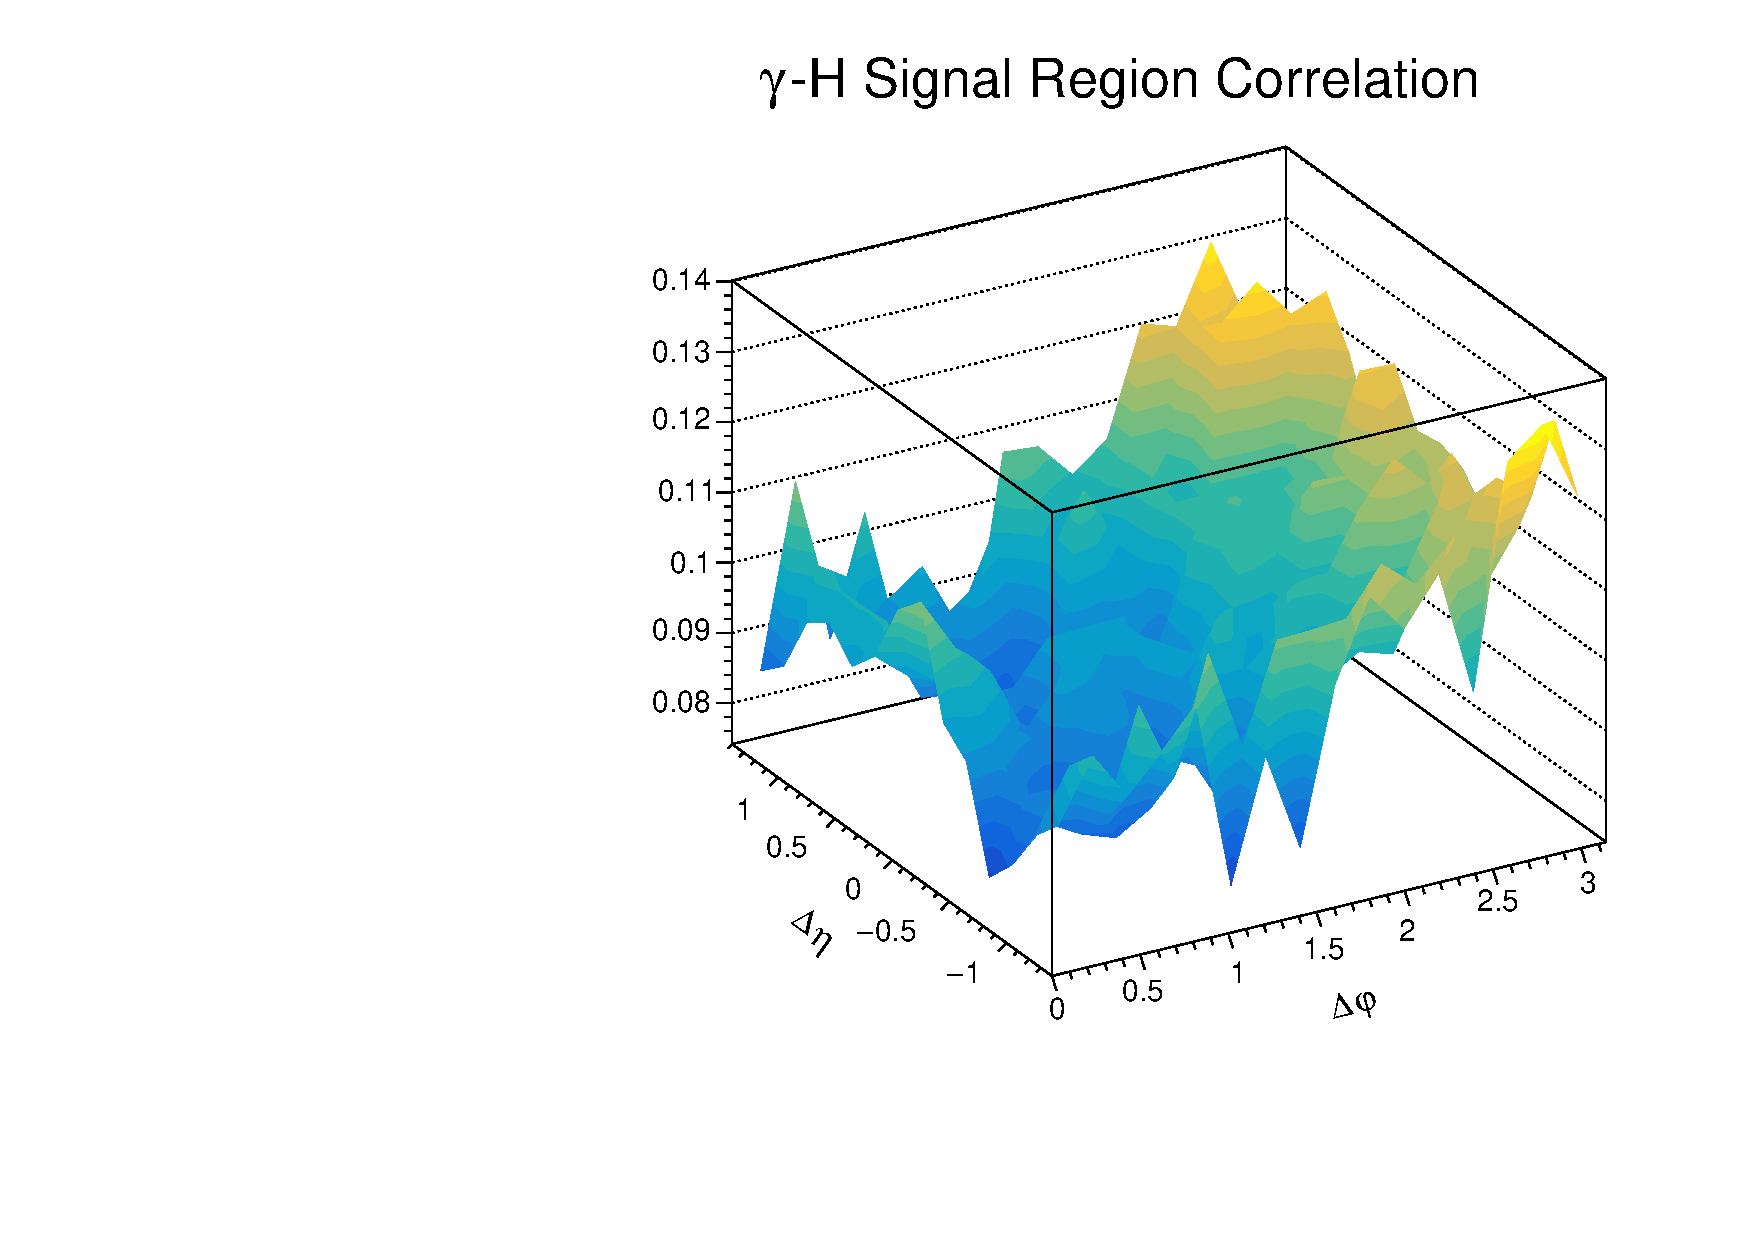
\includegraphics[width = 0.32 \textwidth]{Data_Analysis/G-H_New/2D_SR.pdf}
\caption{\textbf{Left} Mixed Event correlation for a single \zt~bin for gamma-triggered, signal region clusters and hadrons from minimum bias events. \textbf{Middle} 2D Correlation for signal region clusters and hadrons from the same events. \textbf{Right} Signal region correlation function corrected for detector acceptance effects.}
\label{fig:SR_2D}
\end{figure}

Same event correlation functions are divided by the mixed event correlation function within the same \zt~bins, shown for a single \zt~bin in Figure~\ref{fig:SR_2D}. This procedure is carried out identically for clusters in the signal and background shower-shape regions. 

The triangular shape in \deltaeta~is due to the limited acceptance of the ITS and EMCal in psuedorapidity. A useful analogy is the integration of two intersecting square waves that result in a clear triangular signal. The round shape in \deltaphi~is more subtle, however. It is due to the inefficiencies and holes in the ITS, i.e. due to imperfections in the tracking system. This is further discussed in section \ref{sec:ToyMC_Mixing}.

% After the same-event correlation functions 



%Thus, $Y(\Delta \phi, \Delta \eta)$ in equation \ref{eq:Y} relates to $C_{\mathrm{SR}}$ and $C_{\mathrm{BR}}$ from equation \ref{eq:CSRCBR} in the following way:

%\begin{eqnarray}
%Y_S(\Delta \varphi, \Delta \eta) &=& C_{\mathrm{SR}}\\
%Y_B(\Delta \varphi, \Delta \eta) &=& C_{\mathrm{BR}}
%\end{eqnarray}

%Where $Y_{\mathrm{S}}$ is the overall yield per trigger isolated, single  photon correlation %function, and $Y_{\mathrm{B}}$ is the overall yield per trigger isolated  merged cluster correlation function.

%\begin{figure}
%\center
%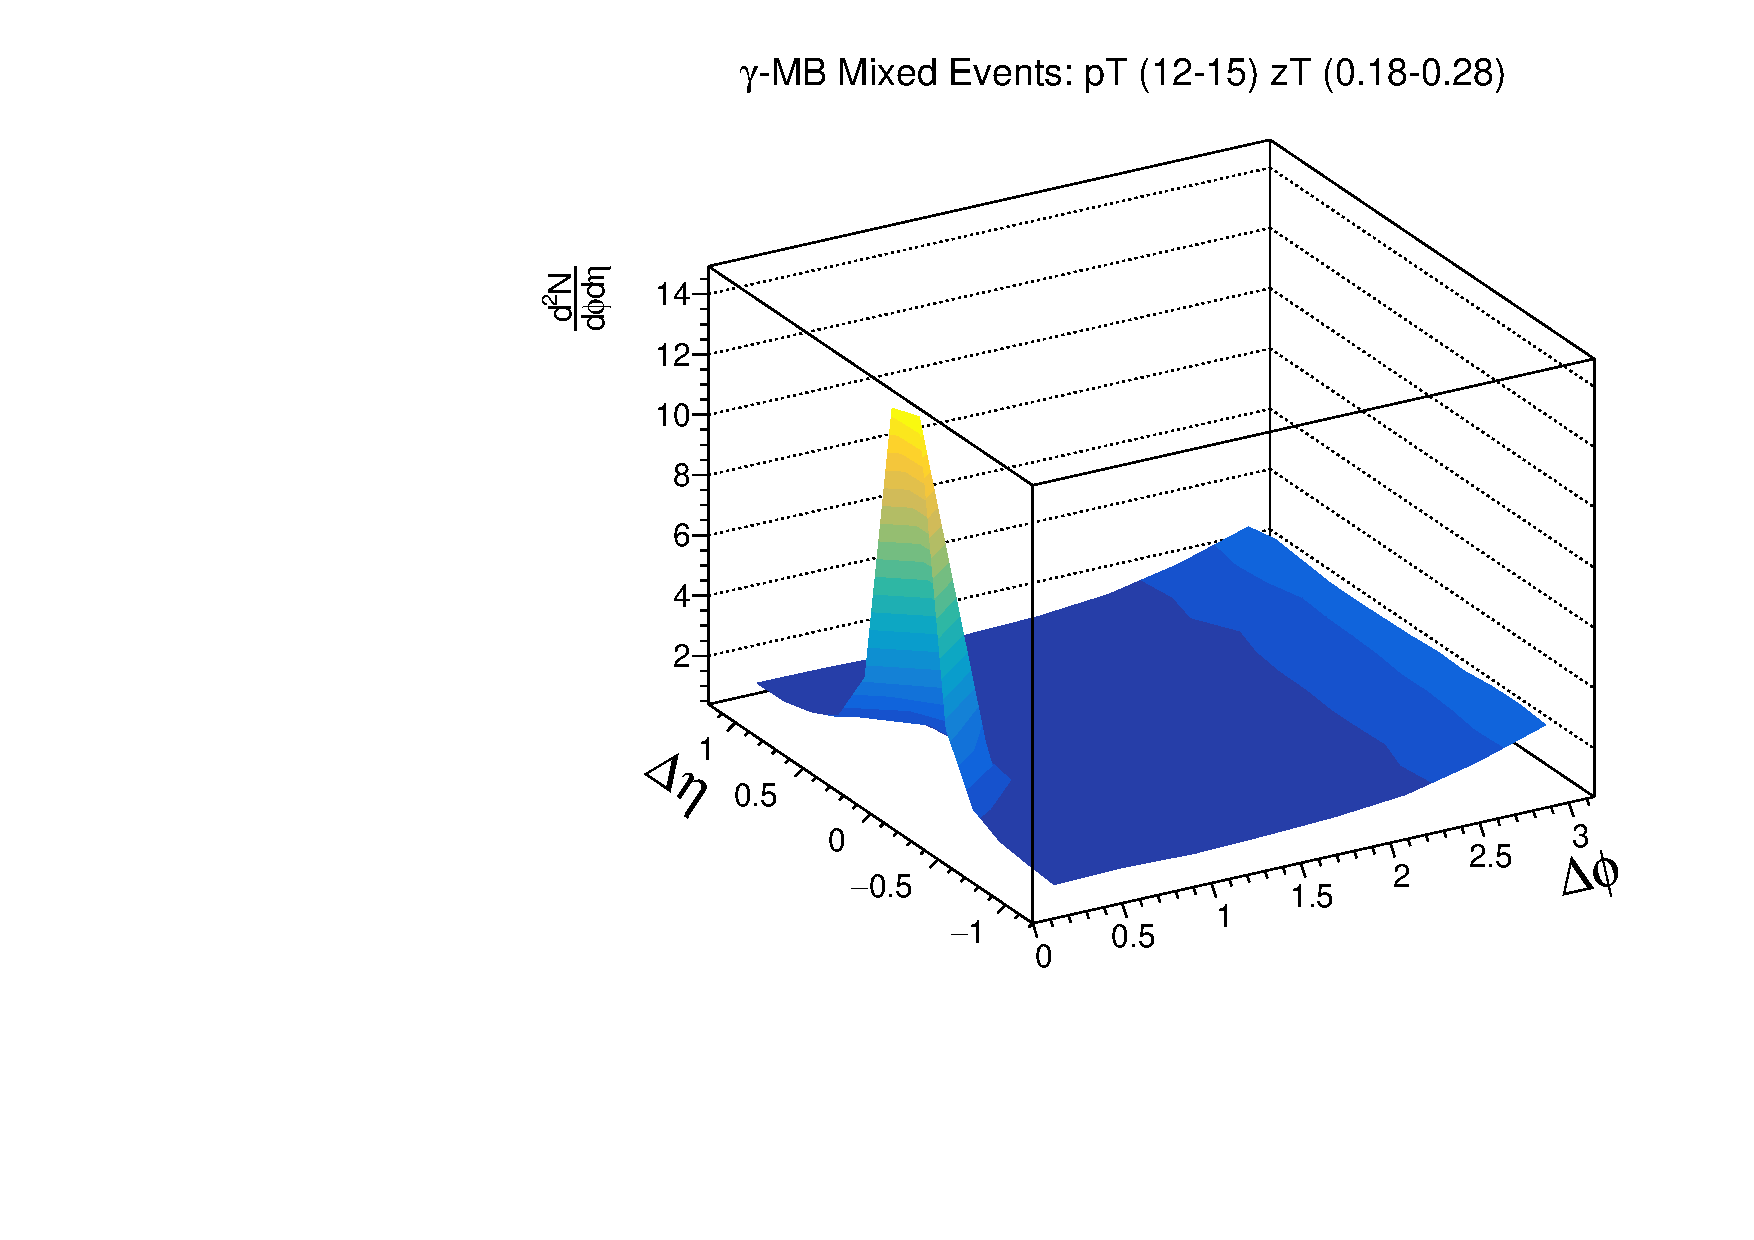
\includegraphics[width=0.49\textwidth]{Data_Analysis/EventMixing/2D_pPb_Corr.pdf}
%\includegraphics[width=0.4\textwidth]{Data_Analysis/EventMixing/13def_Eta_Inclusive.pdf}
%\caption{\textbf{Left}: Correlation function for inclusive photons, after mixed-event correction. \textbf{Right:} $\Delta\eta$ projection from $0 < \Delta\Phi <\frac{\pi}{2}$ of correlation function from a different zT bin. A flat $\Delta\eta$ projection outside of the near side peak is just one indication that detector acceptance effects are corrected for, and informs our estimate for the uncorrelated background. The correlation was normalized such that the maximum value was 1}
%\label{Same_Mix}
%\end{figure}






% At \(\Delta\phi, \Delta\eta\) = (0,0), it is assumed that the trigger and associated particle experience the same detector affects. The mixed event correlation function was therefore normalized to 1 at \(\Delta\phi \Delta\eta\) = (0,0). The overall corrected same event correlation is then given by:


%Too much detail, this is fine for your thesis but for the approval I think we should just show the results. 
%The pseudo code below follows this description, using \(\gamma\) to denote a \(\gamma\)-triggered event, and \(M_B\) to denote a minimum-bias event. The \textit{unrequested} state refers to a \(M_B\) event on a \(\gamma\)-event's preference list that has not yet been requested for pairing.\\

%\FloatBarrier
%\begin{algorithmic}
%\Procedure{GaleShapleyPairing}{}
%\While{\(\exists\) \textit{free} \(\gamma\) with an unrequested \(M_B\) on \(\gamma\)'s list}
%\State \(M_B\) = first unrequested MinBias Event on \(\gamma\)'s list.
%\If {\(M_B\) is free}
%\State (\(\gamma\),\(M_B\)) become paired
%\Else{ some pair (\(\gamma\)',\(M_B\)) exists}%
%	\If{\(M_B\) prefers \(\gamma\) to \(\gamma\)'}
%    \State \(\gamma\)' becomes free
%    \State (\(\gamma\),\(M_B\)) become paired
%    \Else
%    \State (\(\gamma\)',\(M_B\)) remain paired
%    \EndIf
%\EndIf
%\EndWhile
%\EndProcedure
%\end{algorithmic}
%\FloatBarrier

%$\epsilon$ is the single track efficiency described in section \ref{sec:Efficiency_fake_rates}, and $f$ is the fake rate given in Equation \ref{eq:fakes}

%\begin{figure}
%\center
%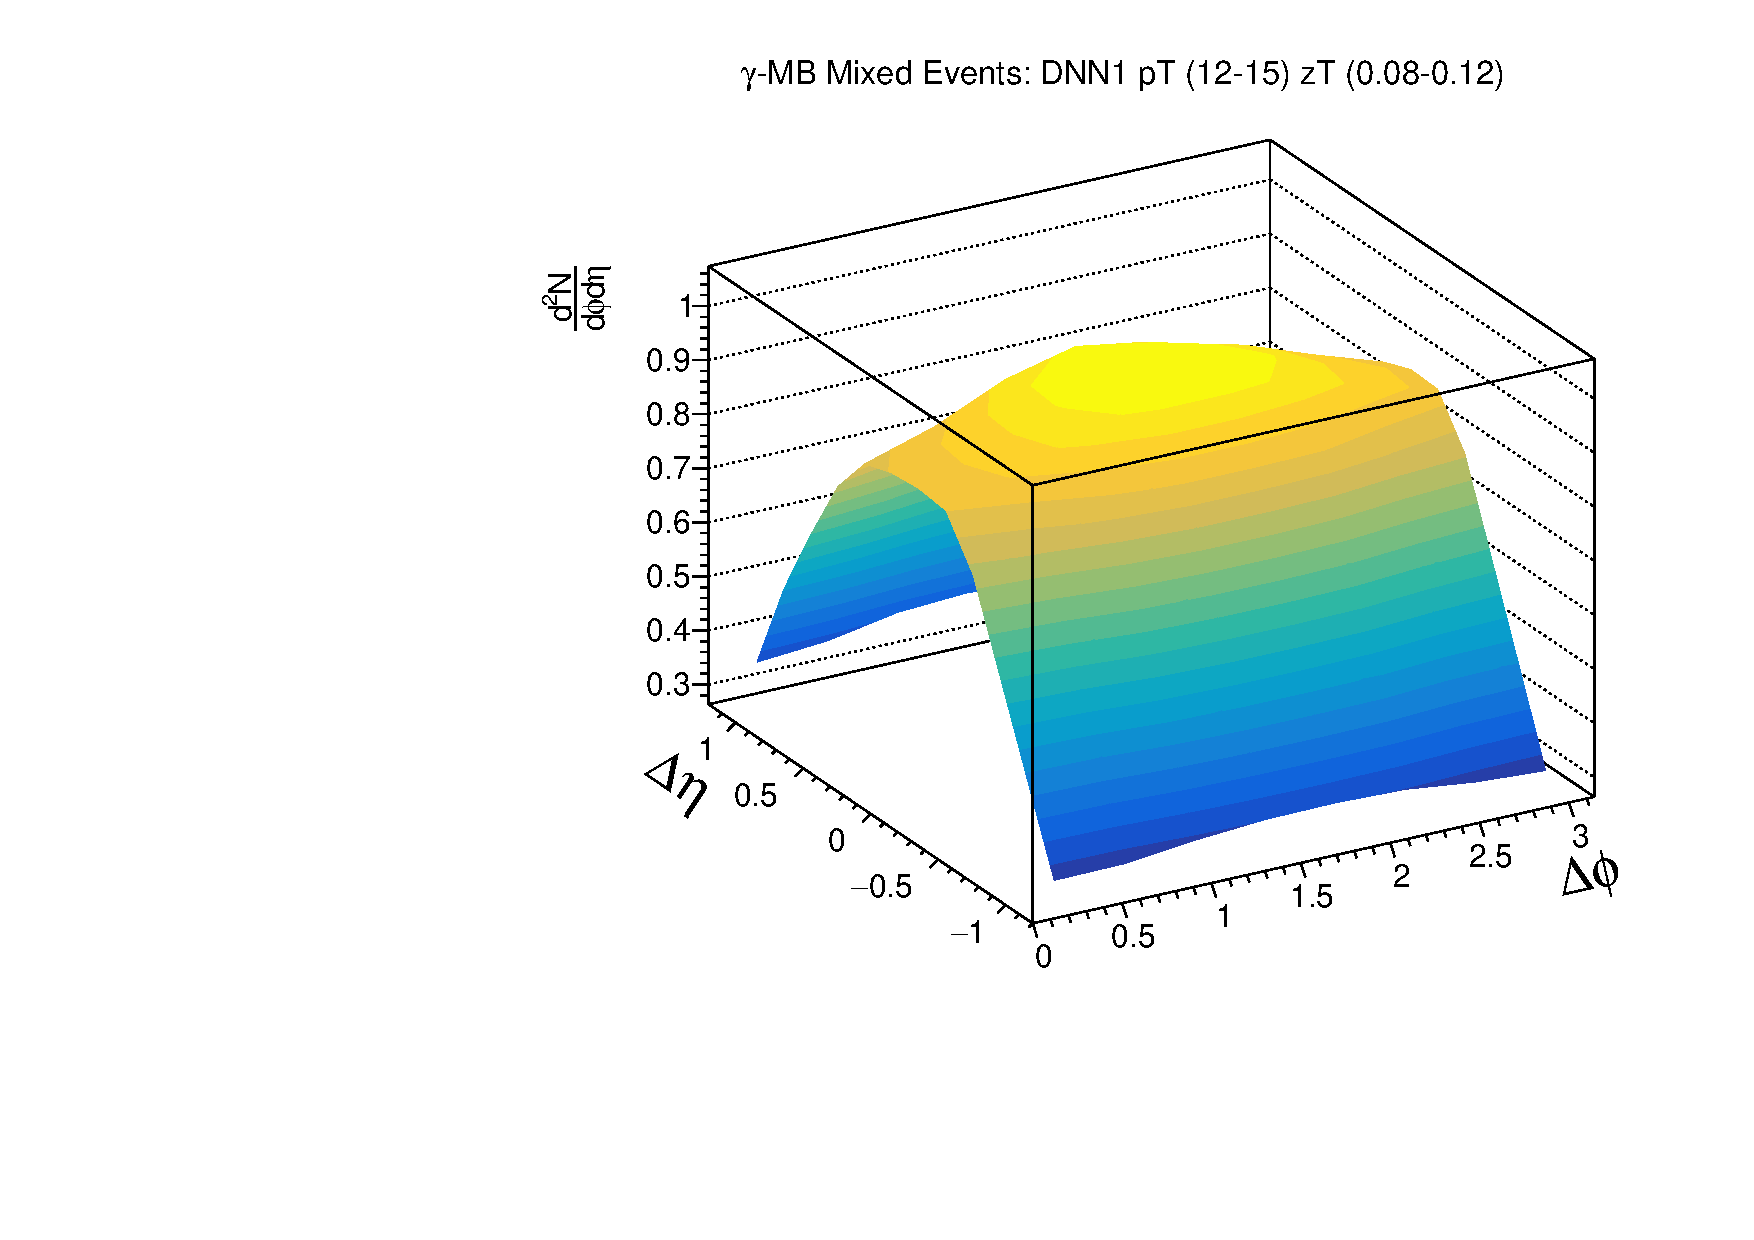
\includegraphics[width=0.495\textwidth]{Data_Analysis/EventMixing/2D_13def_signal_Correlations.pdf}
%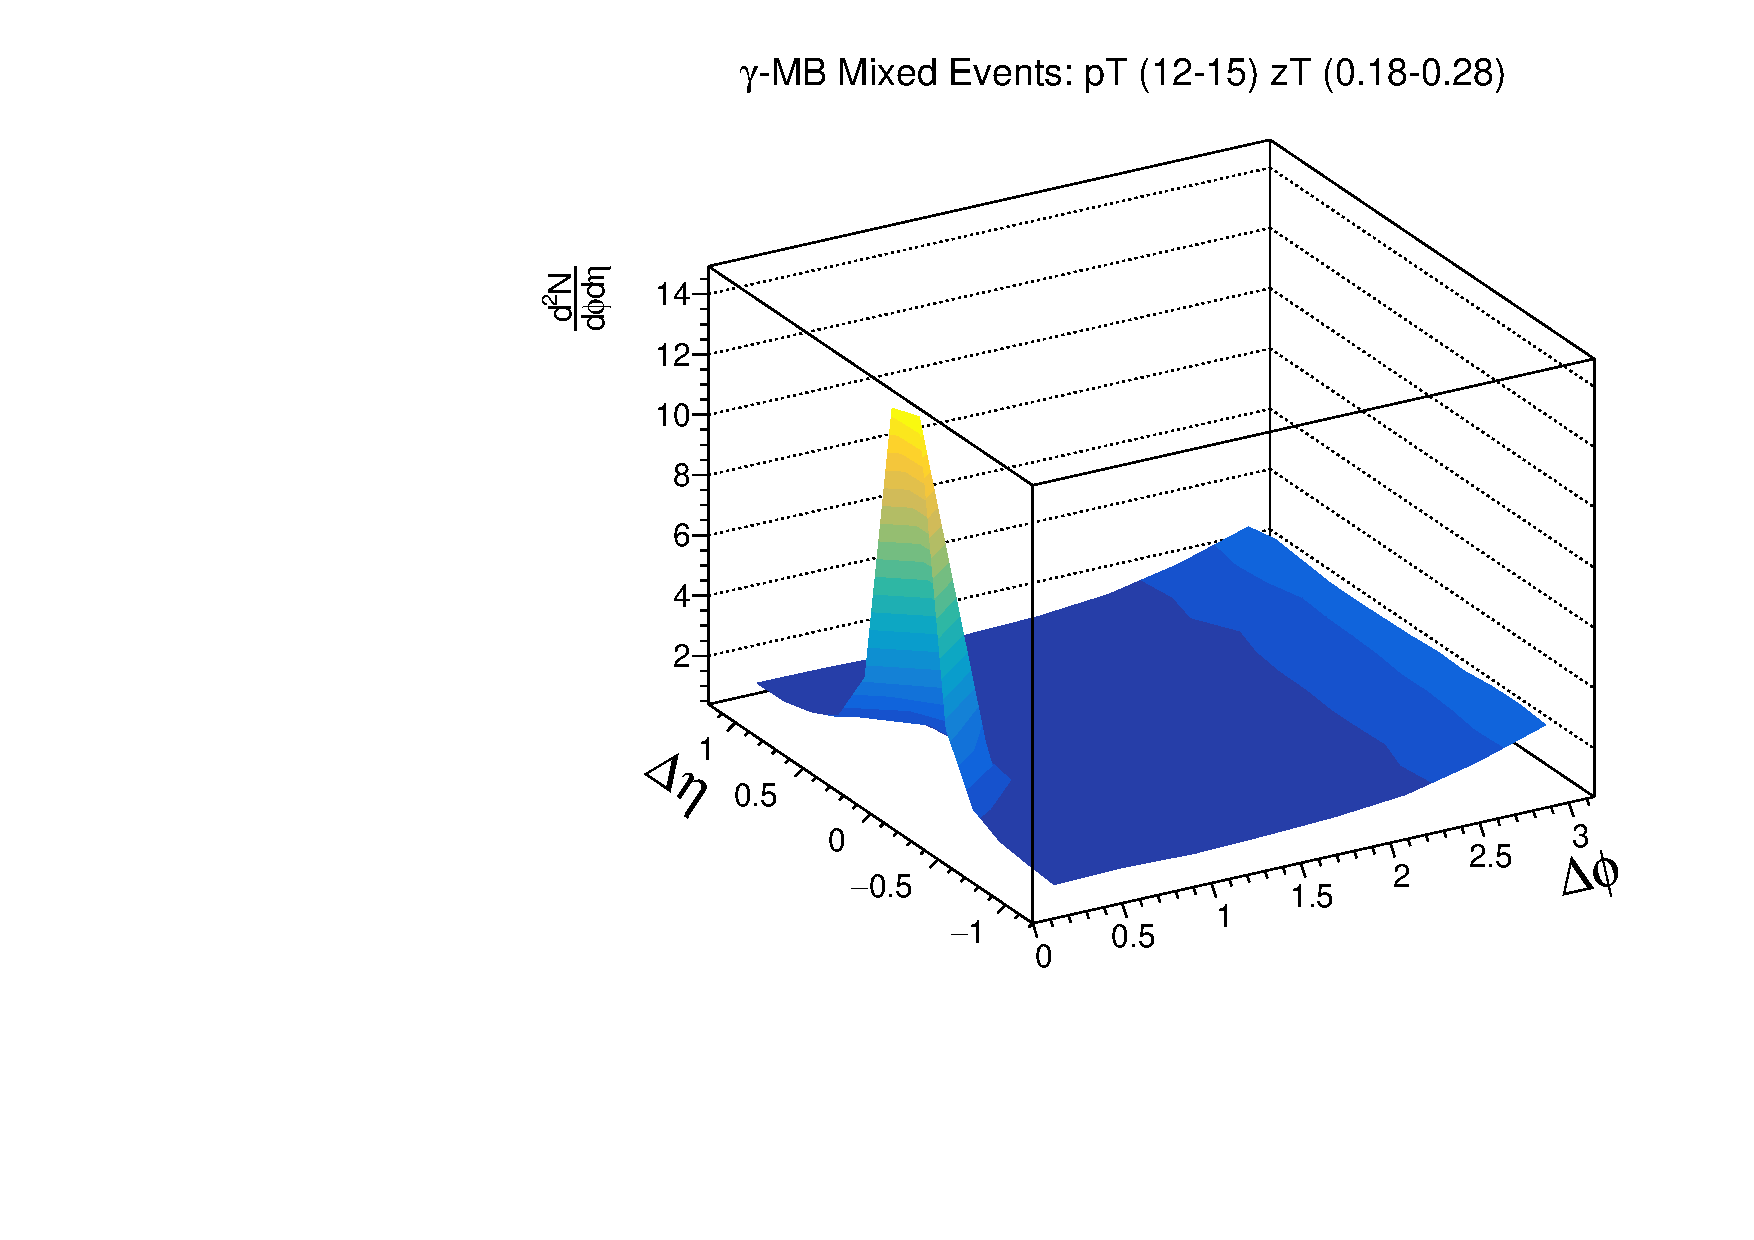
\includegraphics[width=0.495\textwidth]{Data_Analysis/EventMixing/2D_pPb_Corr.pdf}
%\caption{\textbf{Left}:Mixed event correlation for a single $z_T$ bin. The trapezoidal shape in $\Delta\eta$ is due to the convolution of EMCal and ITS acceptances in $\eta$. The non-uniformity in $\Delta\phi$ is attributed to holes in the ITS acceptance. \textbf{Right}: Correlation function for inclusive photons, after mixed-event correction.}
%\label{GS_Mixed_2D}
%\end{figure}

%TODO Get Figures in here
%TODO Decide on using inclusive shapes
%TODO Fix ERrors

\subsection{Fully Corrected \CSR and \CBR}
\label{sec:corrected_correlations}
The fully-corrected \CSR~and \CBR~correlations are shown in Figures~\ref{fig:pp_SR_BR_Overlay_pp} and \ref{fig:pPb_SR_BR_Overlay_pPb}. The shown \gammaiso--hadron correlations are the difference between the scaled-\CSR~and the scaled-\CBR, which are shown in blue and red respectively. While the statistical precision of both \CSR~and \CBR~is high in all \zt~bins and datasets, this gets diluted in the subtraction. That is, the low-purity leads to the subtraction of two comparable numbers, which results in a large statistical uncertainty.

\begin{sidewaysfigure}
\centering   
    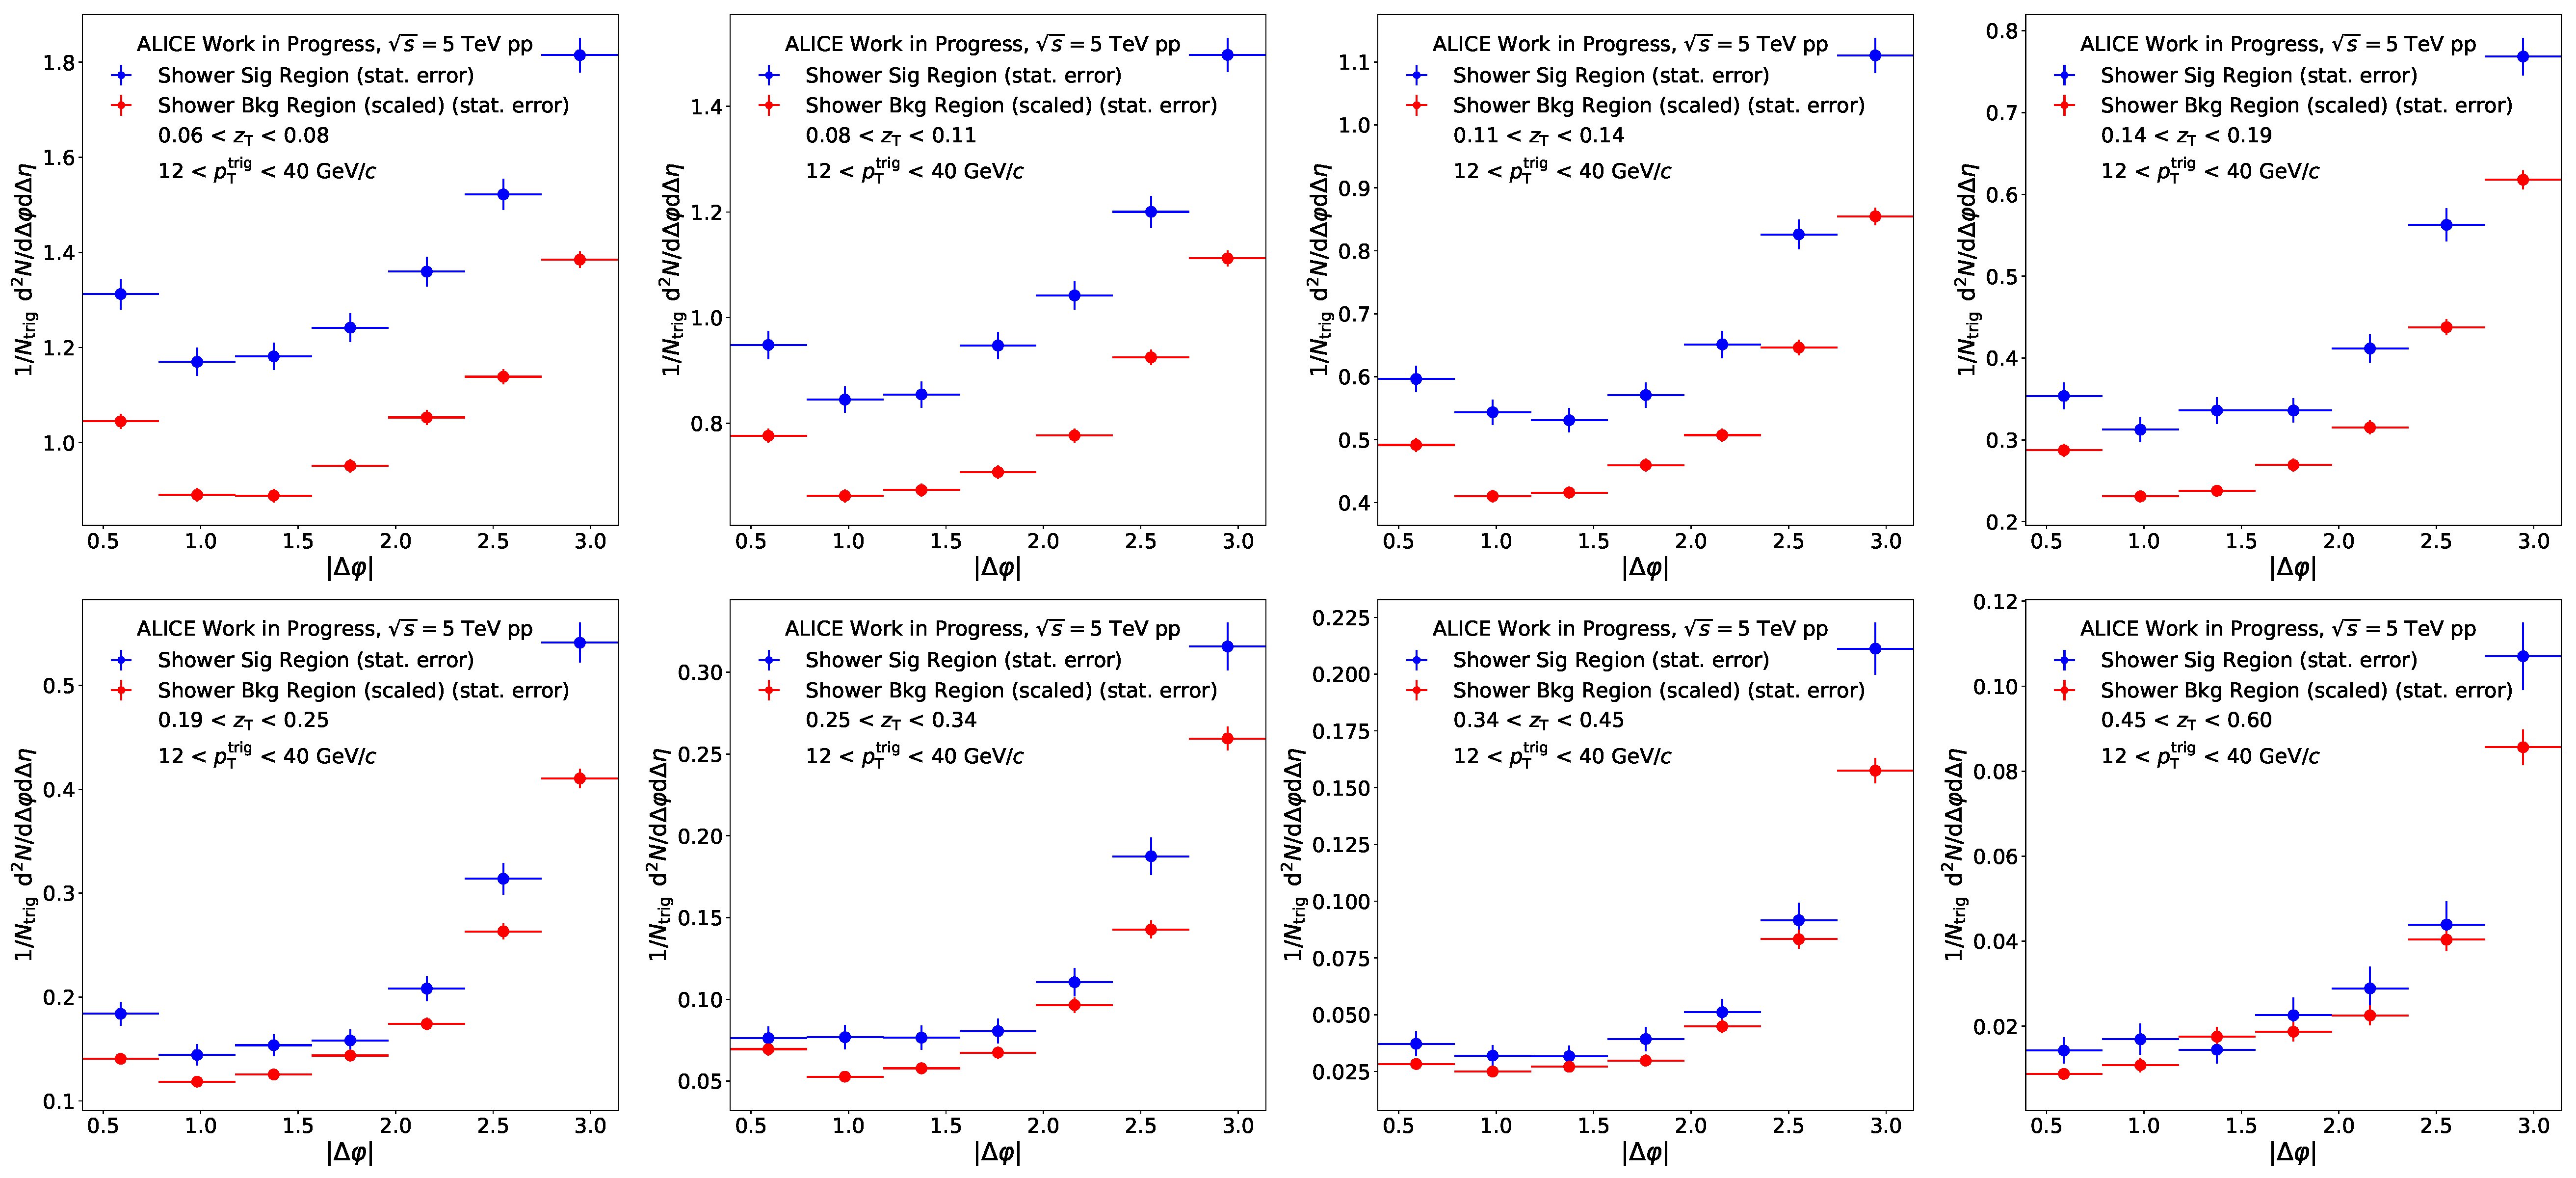
\includegraphics[width = 1.0 \textwidth]{G-H_New/pp_SR_BR_Overlay_pT_0.pdf}
    \caption{Signal-region correlation \CSR~(blue) and background-region correlation \CBR~(red) in pp collisions for various \zt~intervals. The error bars represent statistical uncertainties only.}
    \label{fig:pp_SR_BR_Overlay_pp}
\end{sidewaysfigure}

\begin{sidewaysfigure}
    \centering
    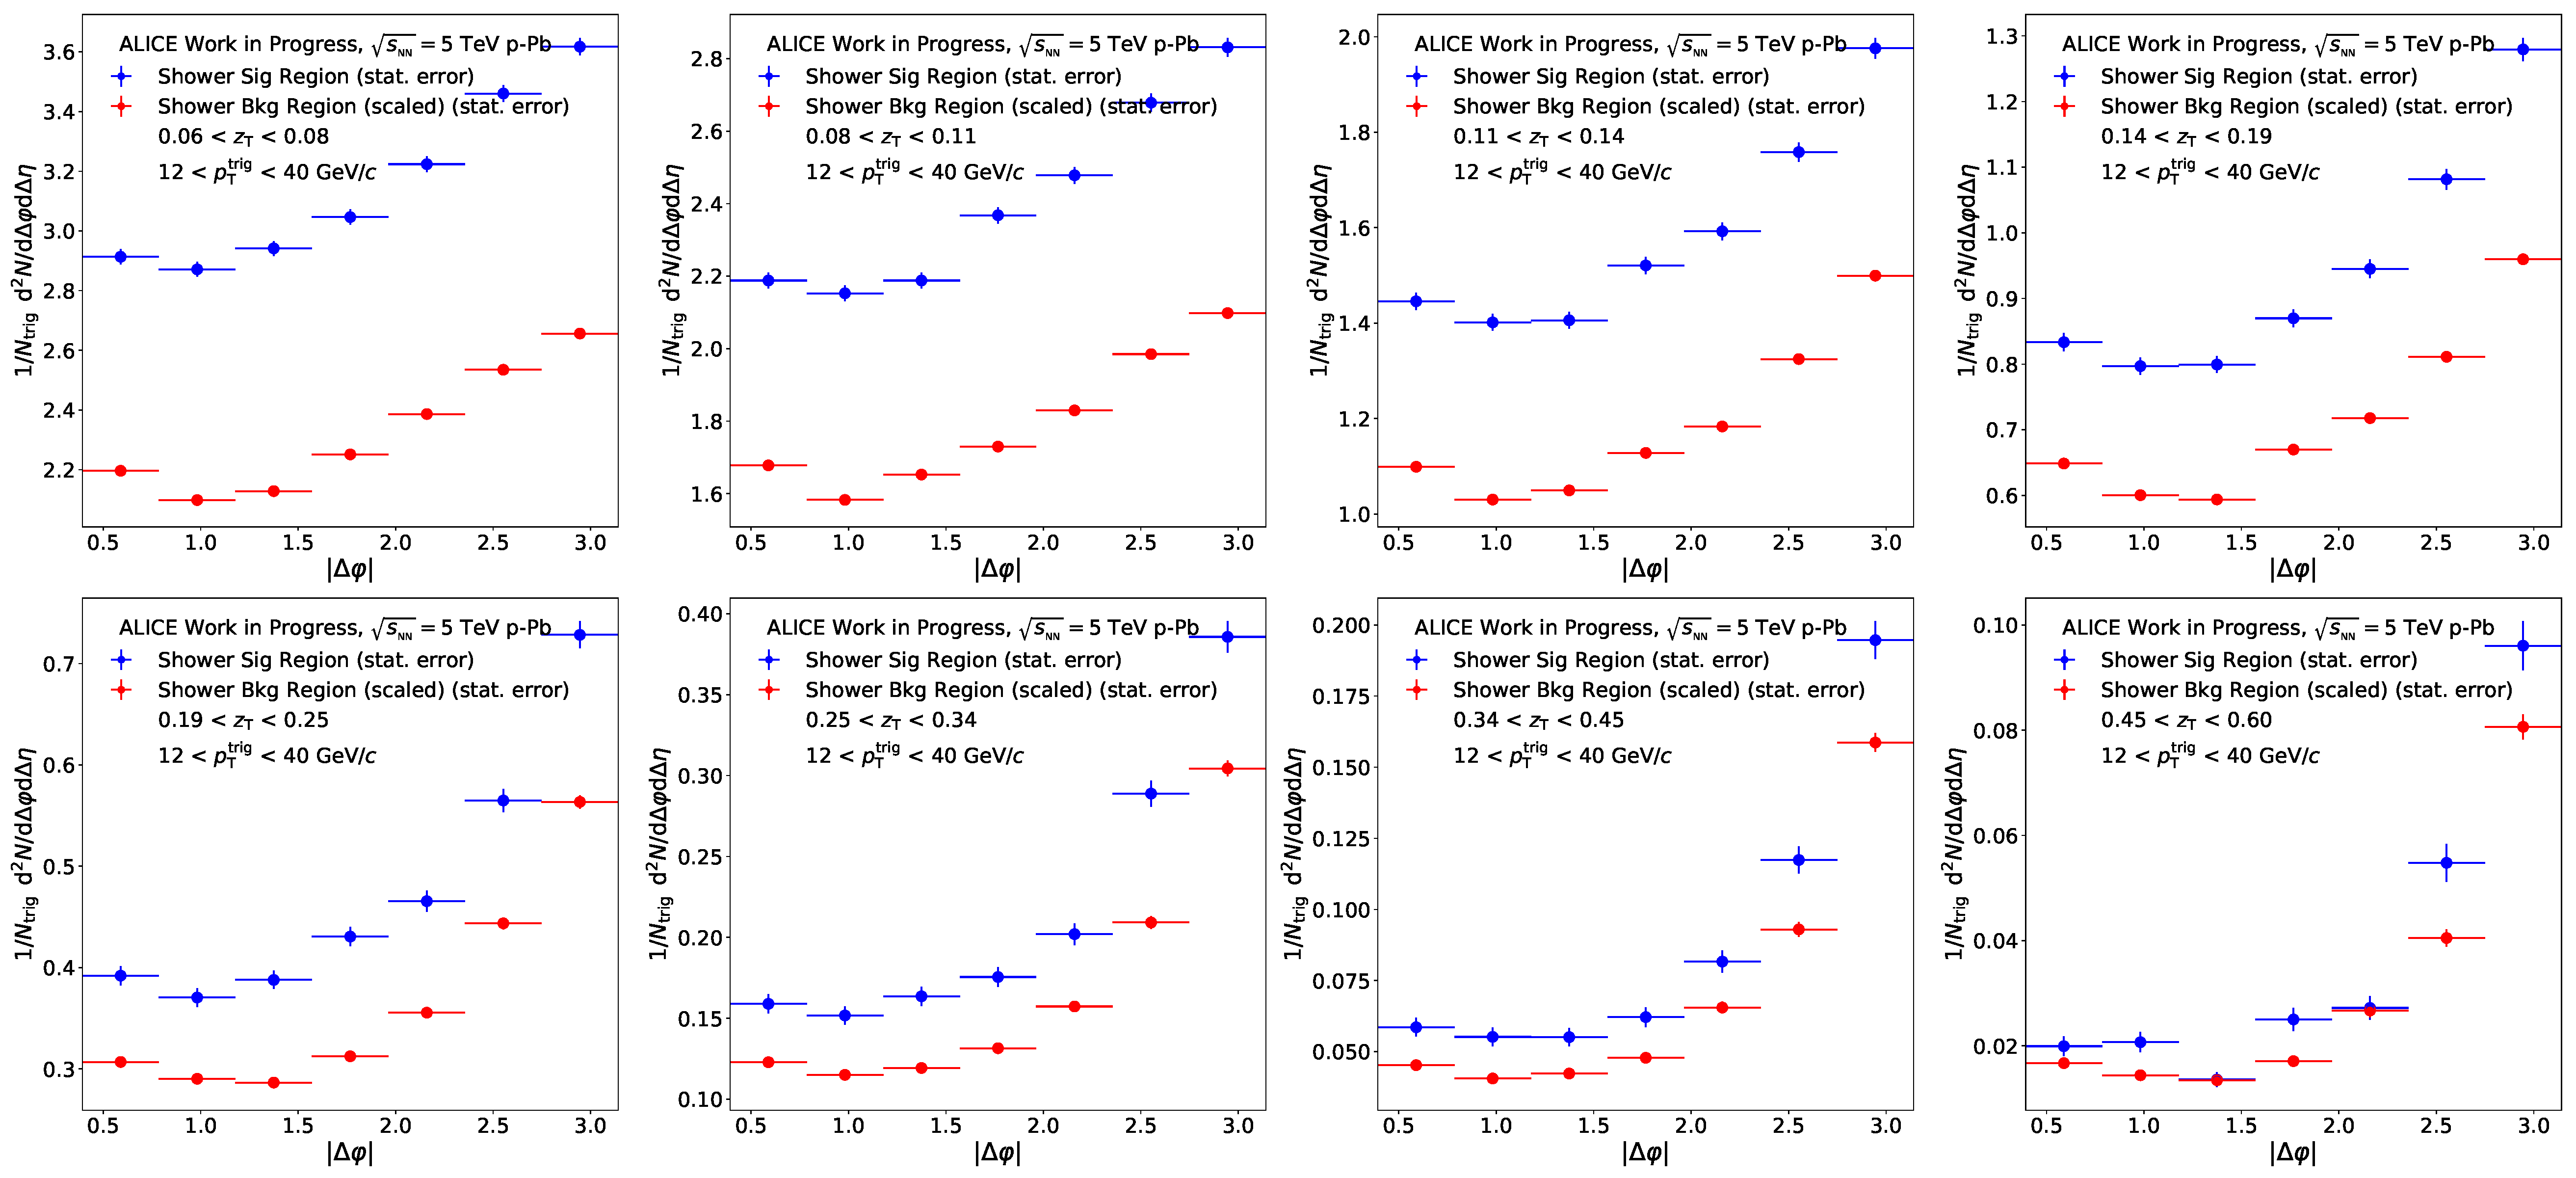
\includegraphics[width = 1.0 \textwidth]{G-H_New/p-Pb_SR_BR_Overlay_pT_0.pdf}
    \caption{Signal-region correlation \CSR~(blue) and background-region correlation \CBR~(red) in \pPb~collisions for various \zt~intervals. The error bars represent statistical uncertainties only.}
    \label{fig:pPb_SR_BR_Overlay_pPb}
\end{sidewaysfigure}
\FloatBarrier


\subsection{Underlying Event Estimation}
\label{sec:ue_subtraction}
As mentioned in Section \ref{sec:ue_isolation}, the underlying event corresponds to all the activity in the event that does not directly relate to the hard scattering in the initial collision. In particular, low \pt hadrons that are not physically correlated with hadronization of the scattered parton make up a large portion of the underlying event. For this reason, this background is also called the \textit{the uncorrelated background}. The first step in this measurement, however, is to take the correlation between the trigger photon and all charged hadrons in the event. There is therefore a large contribution to the measured correlation functions from hadrons in underlying event that must be subtracted.

To subtract this underlying event contribution, we use the zero-yield at minimum method. As the name suggests, this method assumes zero true signal at the minimum of the correlation function [include reference that the referee recently asked for]. The distribution of hadrons arising from the underlying event in pp and in \pPb collisions is conveniently isotropic in $\varphi$. Therefore, the distribution of \deltaphi, the angle between the trigger photon and the charged hadrons from the underlying event, will be flat in \deltaphi. As result, the contribution from the underlying evet can be estimated as a flat pedestal in \deltaphi.

In dihadron and dijet measurements, the minimum occurs most often around \deltaphi = $\pi/2$. This is because a struct parton is kinematically unlikely to scatter at roughly 90 \degree~from another parton in the initial collision. An illustration of this method for \textit{dihadron} measurements is shown in Figure \ref{fig:dihadron_cartoon}.
%FIXME: Fix dihadron cartoon reference (different .tex files)

The isotropic nature of hadrons in the underlying event tells us the shape of the background is a pedestal, while the ZYAM assumption indicates the overall hight of the pedestal. Once the shape and magnitude of the underlying event contribution is understood, this background can be subtracted from the correlation functions. 

In this analysis, however, we use a modified version of the ZYAM method. One of the most prominent features of Figure \ref{fig:dihadron_cartoon} is a near sied peak made up of the autocorrelation of charged hadrons within a jet. The triggers in this analysis, however, are isolated prompt photons that have little to no surrounding hadronic activity.  Therefore, the near side jet peak show in Figure \ref{fig:dihadron_cartoon} is completely absent in isolated prompt photon-hadron correlations. While some surrounding hadronic activity can still be present, either due to fragmentation photons from a jet that are surrounded by the jet constituents, or by decay photons within a jet, the latter is subtracted away by subtracting the decay-photon hadron correlation.

As a result, the minimum of the \gammaiso-hadron correlation function spans a much larger region in \deltaphi~than in the dihadron case. We modify the standar ZYAM method by take the average value of the correlation function in the region of $0.4 < \deltaphi < \pi/2$ to estimate the underlying event pedestal, rather than a much narrower region centered around \deltaphi$\approx \pi/2$.  A minimum \deltaphi~of $0.4$ is used in order to avoid the region of the isolation cone used in the photon isolation calculation -- avoiding an artificially low pedestal estimate. The maximum of $\pi/2$ is used to avoid the tail of the away side jet peak.

This larger region in \deltaphi~has the advantage of higher statistical precision in the underlying event estimate. The magnitude of the underlying event is estimated for both SR and BR correlation functions, and subtracted as constant in \deltaphi. In order to show the effect of pedestal subtraction on the correlation functions in pp and \pPb~data, the correlation functions in both systems are overlayed in Figure~\ref{fig:BF_UE_zT_second} . By construction, the points at small $\Delta\varphi$ are consistent with zero as demonstrated by the dark grey bands. Additionally, the figures demonstrate the larger underlying event in \pPb~data, as well as the agreement in away side yields in the two systems after pedestal subtraction. This also shows visually the fraction of signal to background, particularly at low \zt~in \pPb~collisions.


\begin{sidewaysfigure}[ht]
\centering
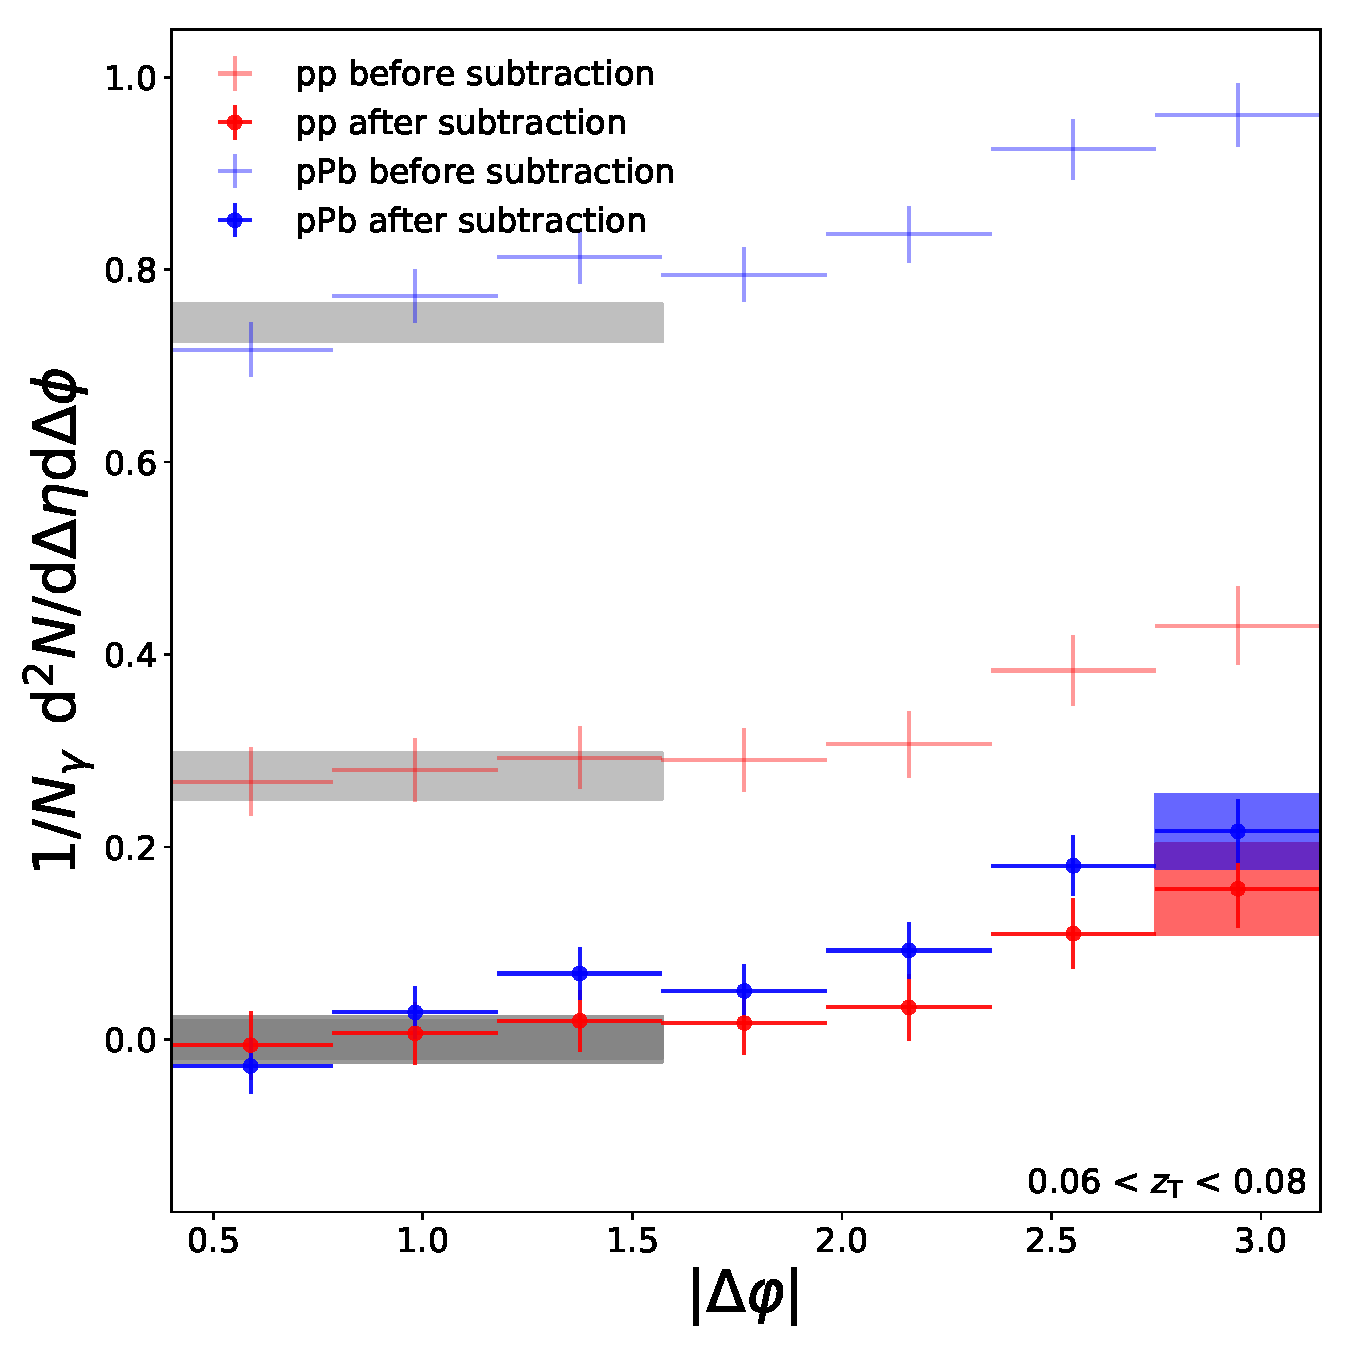
\includegraphics[width = 0.24 \textwidth]{G-H_New/Befor_After_UE_pp-pPb_pT_0_zT_0.pdf}
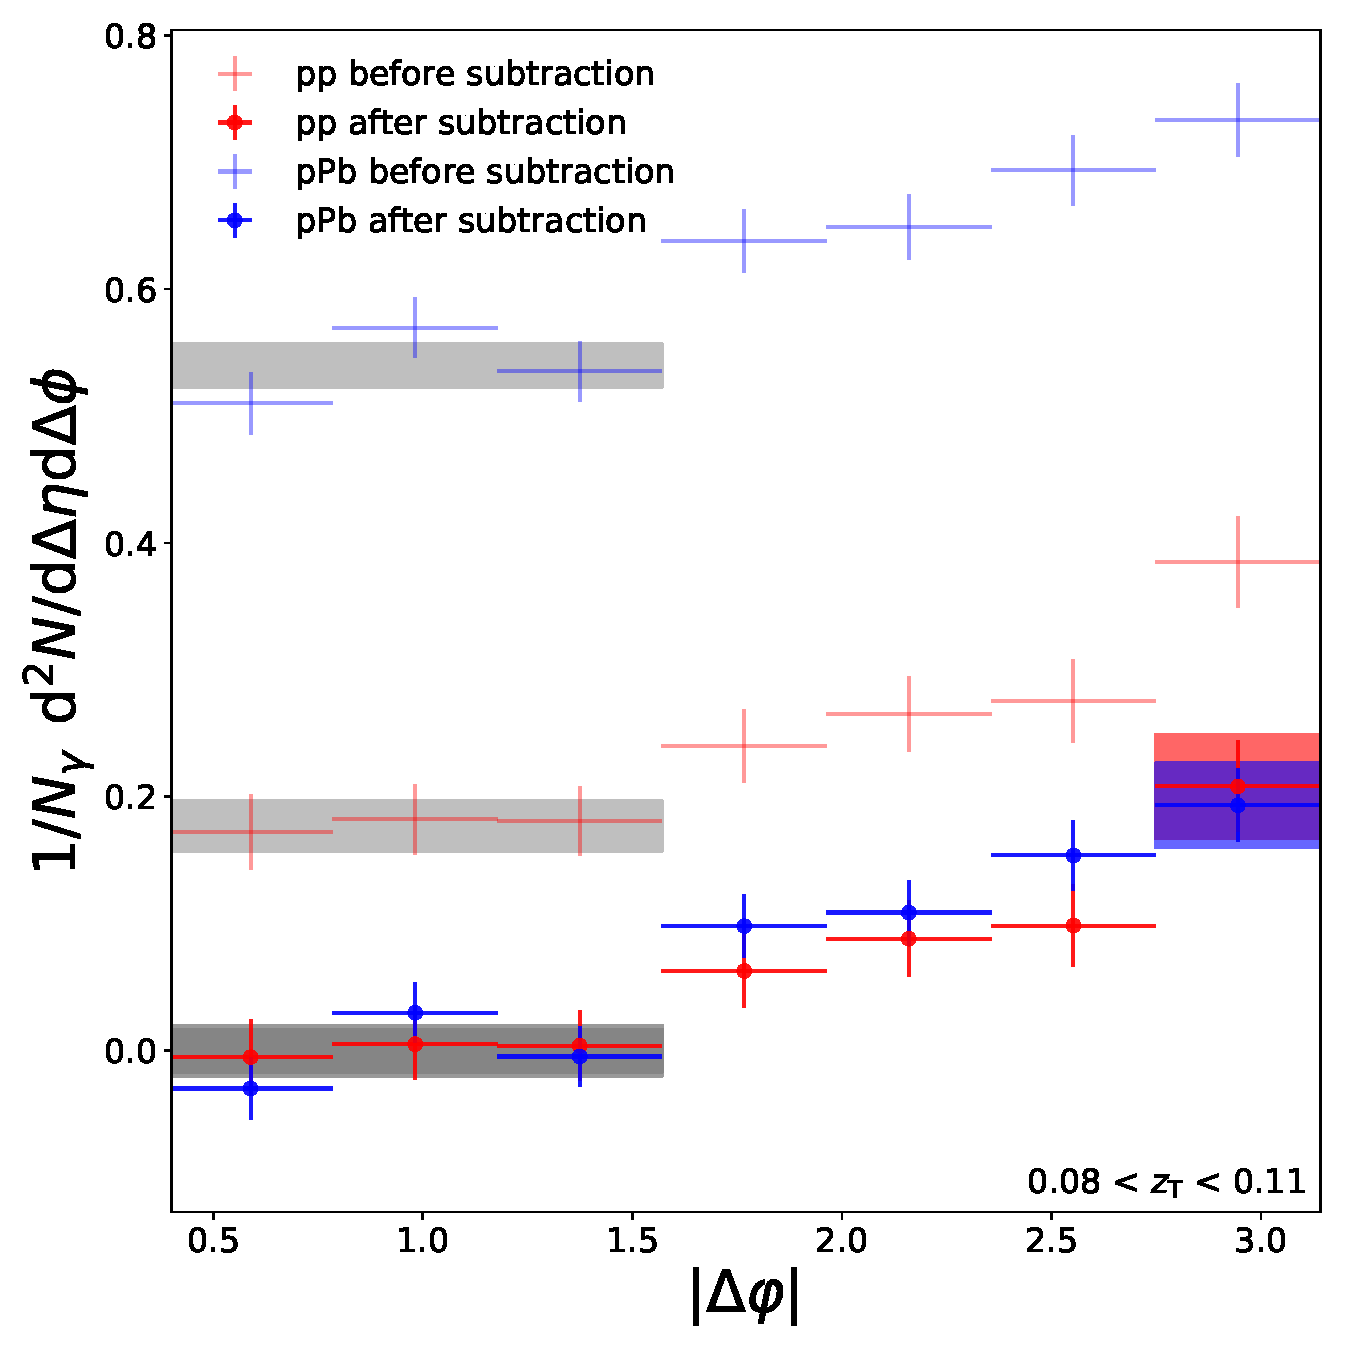
\includegraphics[width = 0.24 \textwidth]{G-H_New/Befor_After_UE_pp-pPb_pT_0_zT_1.pdf}
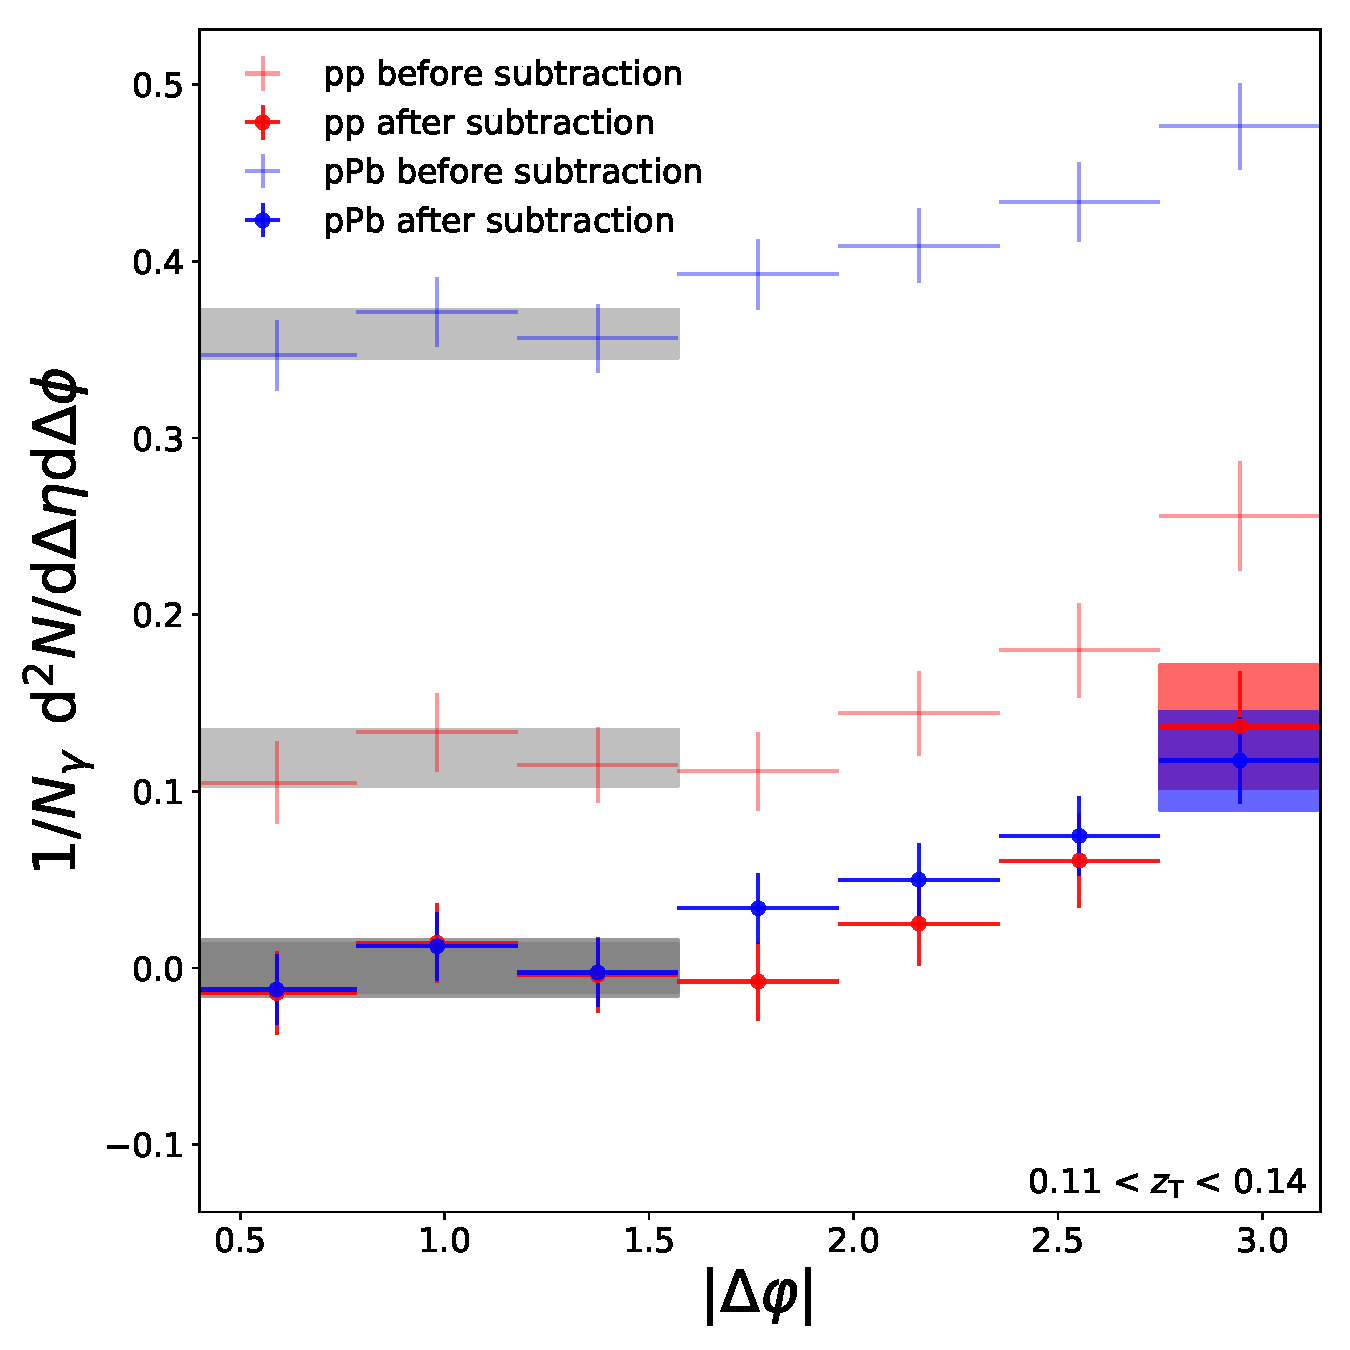
\includegraphics[width = 0.24 \textwidth]{G-H_New/Befor_After_UE_pp-pPb_pT_0_zT_2.pdf}
\includegraphics[width = 0.24 \textwidth]{G-H_New/Befor_After_UE_pp-pPb_pT_0_zT_3.pdf}
\includegraphics[width = 0.24 \textwidth]{G-H_New/Befor_After_UE_pp-pPb_pT_0_zT_4.pdf}
\includegraphics[width = 0.24 \textwidth]{G-H_New/Befor_After_UE_pp-pPb_pT_0_zT_5.pdf}
\includegraphics[width = 0.24 \textwidth]{G-H_New/Befor_After_UE_pp-pPb_pT_0_zT_6.pdf}
\includegraphics[width = 0.24 \textwidth]{G-H_New/Befor_After_UE_pp-pPb_pT_0_zT_7.pdf}
\caption{Correlation functions in pp (red) and \pPb~(blue) before and after pedestal subtraction. The light grey bands represent the ZYAM estimates, while the dark gray bands represent the near side average after subtraction. The colored bands represent the away side average after pedestal subtraction}
\label{fig:BF_UE_zT_second}
\end{sidewaysfigure}

After the pedestal subtraction, one can begin to see the similarities between the correlation functions in pp and \pPb.


\subsection{Fully Subtracted Correlation Functions}
\label{sec:decaybkgsubtraction}
The final $ \gammaiso$-hadron correlations are reported in $\zt$  bins for each trigger-photon $\pt$ bin, where $\zt$ is the ratio of the associated hadron, $\pt^\mathrm{h}$, to isolated photon transverse momentum, $\zt = \pt^{\mathrm{h}}/\pt^{\gammaiso}$. The fully subtracted azimuthal correlations as a function of $ \Delta\varphi$, the azimuthal angle between the photon and the hadron, are shown in Fig.~\ref{fig:GH_Correlations} for pp and \pPb~data. With the measured \gammaiso~ constraining the parton kinematics, the distribution of away-side associated hadrons with momentum fraction \zt represents the fragmentation function of the parton.

\FloatBarrier
 \begin{figure*}
     \centering
     \includegraphics[width=0.3\textwidth]{Data_Analysis/gammahadron/Cs_Final_Indv_pT_0_zT_0.pdf}
    \includegraphics[width=0.3\textwidth]{Data_Analysis/gammahadron/Cs_Final_Indv_pT_0_zT_1.pdf}        
    \includegraphics[width=0.3\textwidth]{Data_Analysis/gammahadron/Cs_Final_Indv_pT_0_zT_2.pdf}        
    \includegraphics[width=0.3\textwidth]{Data_Analysis/gammahadron/Cs_Final_Indv_pT_0_zT_3.pdf}        
    \includegraphics[width=0.3\textwidth]{Data_Analysis/gammahadron/Cs_Final_Indv_pT_0_zT_4.pdf}        
    \includegraphics[width=0.3\textwidth]{Data_Analysis/gammahadron/Cs_Final_Indv_pT_0_zT_5.pdf}        
    \includegraphics[width=0.3\textwidth]{Data_Analysis/gammahadron/Cs_Final_Indv_pT_0_zT_6.pdf}        
    \includegraphics[width=0.3\textwidth]{Data_Analysis/gammahadron/Cs_Final_Indv_pT_0_zT_7.pdf}
    \caption{$\gammaiso$--hadron correlation functions for pp (red) and \pPb~(blue) data at $\sqrt{s_\mathrm{NN}}$ = 5.02 TeV as measured by the ALICE detector. The different panels represent three different \zt~bins. The correlation functions are projected over the range $|\Delta\eta| < 1.2$. The darker bands at zero represents the uncertainty from the underlying event estimation in pp and \pPb. The underlying event was estimated over the range $0.4 <|\Delta\varphi| < 1.6$. The vertical bars represent statistical uncertainties only. The boxes indicate the systematic uncertainties. The dashed green line represents the \gammaiso--hadron correlation function obtained with \textsc{PYTHIA 8.2} Monash Tune. ``$p$" is the p-value for the hypothesis that the pp and \pPb data follow the same true correlation function.
    }
     \label{fig:GH_Correlations}
 \end{figure*}

%\begin{figure*}
    %\centering
    %\includegraphics[width=1.0\textwidth]{gammahadron/Cs_Final_All_pT_0.pdf}        
    %\caption{$\gammaiso$--hadron correlation functions for pp (red) and \pPb~(blue) data at $\sqrt{s_\mathrm{NN}}$ = 5.02 TeV as measured by the ALICE detector. The different panels represent different \zt~bins. The purple band represents the uncertainty from the underlying event estimate n pp and \pPb. The vertical bars represent statistical uncertainty only. The horizontal bars represent the bin width in $\Delta\varphi$. The histogram is the \gammaiso--hadron correlation function obtained with \textsc{PYTHIA 8.2} Monash Tune. "p" is the p-value for the hypothesis that the pp and p-Pb data follow the same true correlation function}
%\end{figure*}

The darker colored bands at zero represents the uncertainty from the uncorrelated background estimate. The vertical bars indicate the statistical uncertainty only. The final correlation functions in each collision system demonstrate similar behavior: both show a signal consistent with zero at small $\Delta\varphi$, and a rising away-side peak at large $\Delta\varphi$ arising predominantly from the hard-scattered parton opposite to the trigger photon.
%$\gammaiso$.

Agreement within uncertainties between pp, \pPb, and the \textsc{PYTHIA 8.2} Monash Tune is observed.
By measuring associated hadrons, correlations can be observed at much larger angles than would otherwise be possible for hadrons within a reconstructed jet. A $\chi^2$ test between pp and \pPb~data and a p-value is calculated in each \zt bin for the null hypothesis that pp and \pPb data follow the same true correlation function. In each bin, the null hypothesis cannot be rejected, indicating that there is no significant difference between the correlation functions in the two collision systems.

\section{Parton Fragmentation Function}
Similar to the methods described in Sec.~\ref{sec:intro_gj} and Sec.~\ref{sec:intro_gh}, the correlation functions from Fig. \ref{fig:GH_Correlations} are then integrated in the region $|\Delta\varphi| > \frac{7\pi}{8}$ for each $\zt$ bin in order to obtain the $\gammaiso$-tagged fragmentation function shown in Fig. \ref{fig:Fragmentation_Functions}. This range roughly corresponds to the azimuthal angle consistent with the commonly used radius of $R=$ 0.4 for jet measurements.

\begin{figure}
    \centering
    \includegraphics[width=0.67\textwidth]{Data_Analysis/gammahadron/Final_FFunction_and_Ratio.pdf}
    \caption{$\gammaiso$-tagged fragmentation function for pp (red) and \pPb~data (blue) at $\sqrt{s_\mathrm{NN}}$ = 5.02 TeV as measured by the ALICE detector. The boxes represent the systematic uncertainties while the vertical bars indicate the statistical uncertainties. The dashed green line corresponds to \textsc{PYTHIA 8.2}. The $\chi^2$ test for the comparison of pp and \pPb~data incorporates correlations among different \zt~intervals. A constant that was fit to the ratio including statistical and systematic uncertainties is shown as grey band, with the width indicating the uncertainty on the fit.}
    \label{fig:Fragmentation_Functions}
\end{figure}

The statistical uncertainty on the away-side yields in each $\zt$ bin is calculated from the statistical uncertainty in the fully subtracted correlation functions, along with the statistical uncertainty arising from the uncorrelated background subtraction. A maximum charged hadron \pt of 10 \GeVc and a photon trigger \pt up to 40 \GeVc could result in a potential bias of the associated \zt spectrum. However, by repeating the analysis in different photon trigger \pt bins, it was found that any such effects were negligible compared to other uncertainties. The two largest sources of systematic uncertainty are from the purity and the single track correction factors. For the chosen $\pt^{\mathrm{track}}$ interval, there is no strong $\pt$ dependence for the uncertainty of the charged tracking efficiency.

 The ratio of the fragmentation functions in \pPb~ and pp collisions is shown in the lower panel of Fig.~\ref{fig:Fragmentation_Functions}.
The fit yields a constant factor of $0.84\pm0.11\mathrm{(stat)}\pm0.19\mathrm{(sys)}$. %with a reduced $\chi^{2}$ of 0.84.  
 Thus, within total uncertainties,
 %ranging from 22--40\% for different \zt~bins
 the \pPb to pp ratio is consistent with unity. %Thus, within approximately 23--40\% these uncertainties, the fragmentation function in \pPb collisions is the same as in pp collisions.



\subsection{\pPb to pp ratio}
\subsection{Integration Window}

\subsection{Cold nuclear matter measurements at future EIC}
\subsection{Transverse Momentum Dependent Distributions}
\subsection{Probing $\hat{q}$ at the EIC}
\subsection{An All-Sillicon Tracker for Jet Measurements at the EIC}
\subsection{Charged Jet Fragmentation Function}
\subsection{Electron-Jet Correlations}
\cite{Fantoni_2011}
%\section{Photon Selection}

